\title{}

%\author{oGs\_ MousE \& Dracs von Mordenheim}


%\date{\today}

\documentclass[8pt]{memoir} %, twocolumn

  
%\usepackage[cm]{fullpage}
\usepackage[a4paper]{geometry}
\usepackage{wrapfig}
\usepackage{multicol}
\usepackage{graphicx}
\usepackage{changepage}
\usepackage{wallpaper}
\usepackage{pdfpages}


\usepackage{fancyhdr}

\usepackage{xcolor}
\usepackage{afterpage}

%\usepackage{fancyhdr}
%\pagestyle{fancy}

\usepackage[pdftex,bookmarks=true]{hyperref}

\newlength{\mylen}
\addtolength{\mylen}{\textheight}
\addtolength{\mylen}{-16pt}
\renewcommand{\familydefault}{\sfdefault}

\setsecnumdepth{chapter}



\begin{document}
%\maketitle

\frontmatter

\newenvironment{changemargin}[2]{%
\begin{list}{}{%
\setlength{\topsep}{0pt}%
\setlength{\leftmargin}{#1}%
\setlength{\rightmargin}{#2}%
\setlength{\listparindent}{\parindent}%
\setlength{\itemindent}{\parindent}%
\setlength{\parsep}{\parskip}%
}%
\item[]}{\end{list}}


% Make one image take up the entire slide content area in beamer,.:
% centered/centred full-screen image, with title:
% This uses the whole screen except for the 1cm border around it
% all. 128x96mm
\newcommand{\titledFrameImage}[2]{
\begin{frame}{#1}
%\begin{changemargin}{-1cm}{-1cm}
\begin{center}
\includegraphics[width=108mm,height=\textheight,keepaspectratio]{#2}
\end{center}
%\end{changemargin}
\end{frame}
}

% Make one image take up the entire slide content area in beamer.:
% centered/centred full-screen image, no title:
% This uses the whole screen except for the 1cm border around it
% all. 128x96mm
\newcommand{\plainFrameImage}[1]{
\begin{frame}[plain]
%\begin{changemargin}{-1cm}{-1cm}
\begin{center}
\includegraphics[width=108mm,height=76mm,keepaspectratio]{#1}
\end{center}
%\end{changemargin}
\end{frame}
}

% Make one image take up the entire slide area, including borders, in beamer.:
% centered/centred full-screen image, no title:
% This uses the entire whole screen
\newcommand{\maxFrameImage}[1]{
\begin{frame}[plain]
\begin{changemargin}{-1cm}{-1cm}
\begin{center}
\includegraphics[width=\paperwidth,height=\paperheight,keepaspectratio]{#1}
\end{center}
\end{changemargin}
\end{frame}
}



%%%%%%%%%%%%%%%%%%%%%%%%%%%%%%%%%%%%%%%%%%%%%%%%%%%%%%%%%%%%%%%%%%%%%%%%%%%%%%%%%%%%%%%%%%%


%%%%%%%%%%%%%%%%%%%%%%%%%% TITLE PAGE %%%%%%%%%%%%%%%%%%%%%%%%%%%%%%%%%%%%%%%%%%%%%%%%%%%%


%%%%%%%%%%%%%%%%%%%%%%%%%%%%%%%%%%%%%%%%%%%%%%%%%%%%%%%%%%%%%%%%%%%%%%%%%%%%%%%%%%%%%%%%%%%

%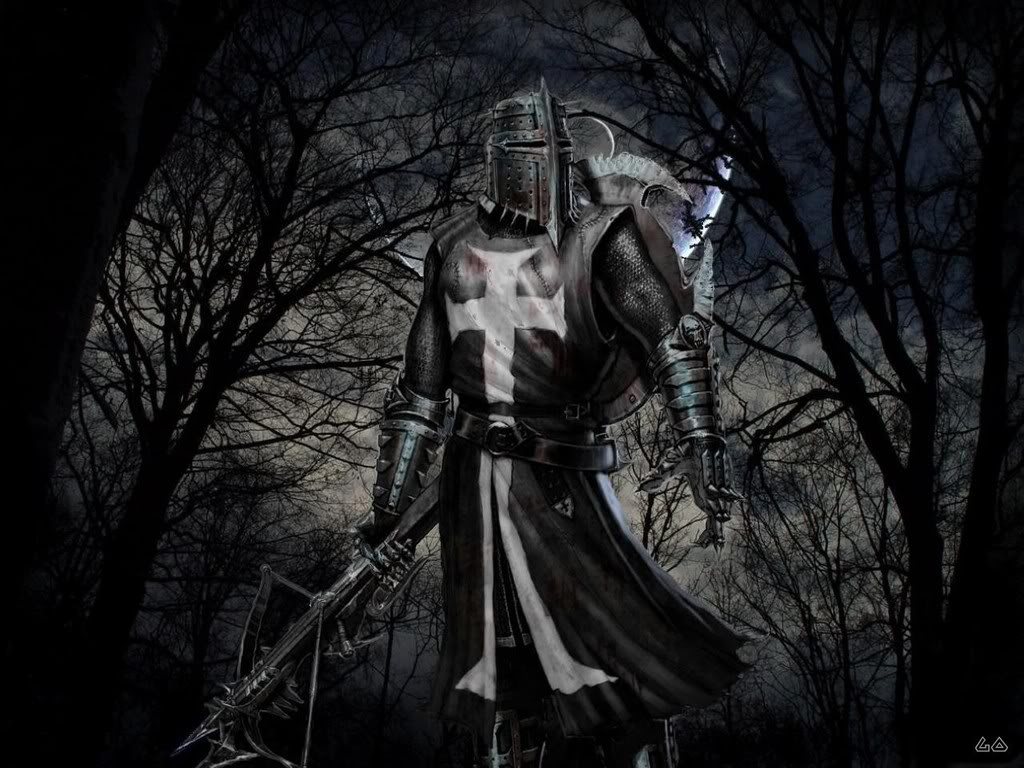
\includegraphics{black_knight}

\newgeometry{left=0cm,top=0cm,right=0cm}

\maxFrameImage{black_knight}
\pagecolor{black}\afterpage{\nopagecolor}
\clearpage
\restoregeometry

%%%%%%%%%%%%%%%%%%%%%%%%%%%%%%%%%%%%%%%%%%%%%%%%%%%%%%%%%%%%%%%%%%%%%%%%%%%%%%%%%%%%%%%%%%%


%%%%%%%%%%%%%%%%%%%%%%%%%% CREDITS PAGE %%%%%%%%%%%%%%%%%%%%%%%%%%%%%%%%%%%%%%%%%%%%%%%%%%%%


%%%%%%%%%%%%%%%%%%%%%%%%%%%%%%%%%%%%%%%%%%%%%%%%%%%%%%%%%%%%%%%%%%%%%%%%%%%%%%%%%%%%%%%%%%%


\newpage

\pagecolor{gray}\afterpage{\nopagecolor}

%\begin{figure}
%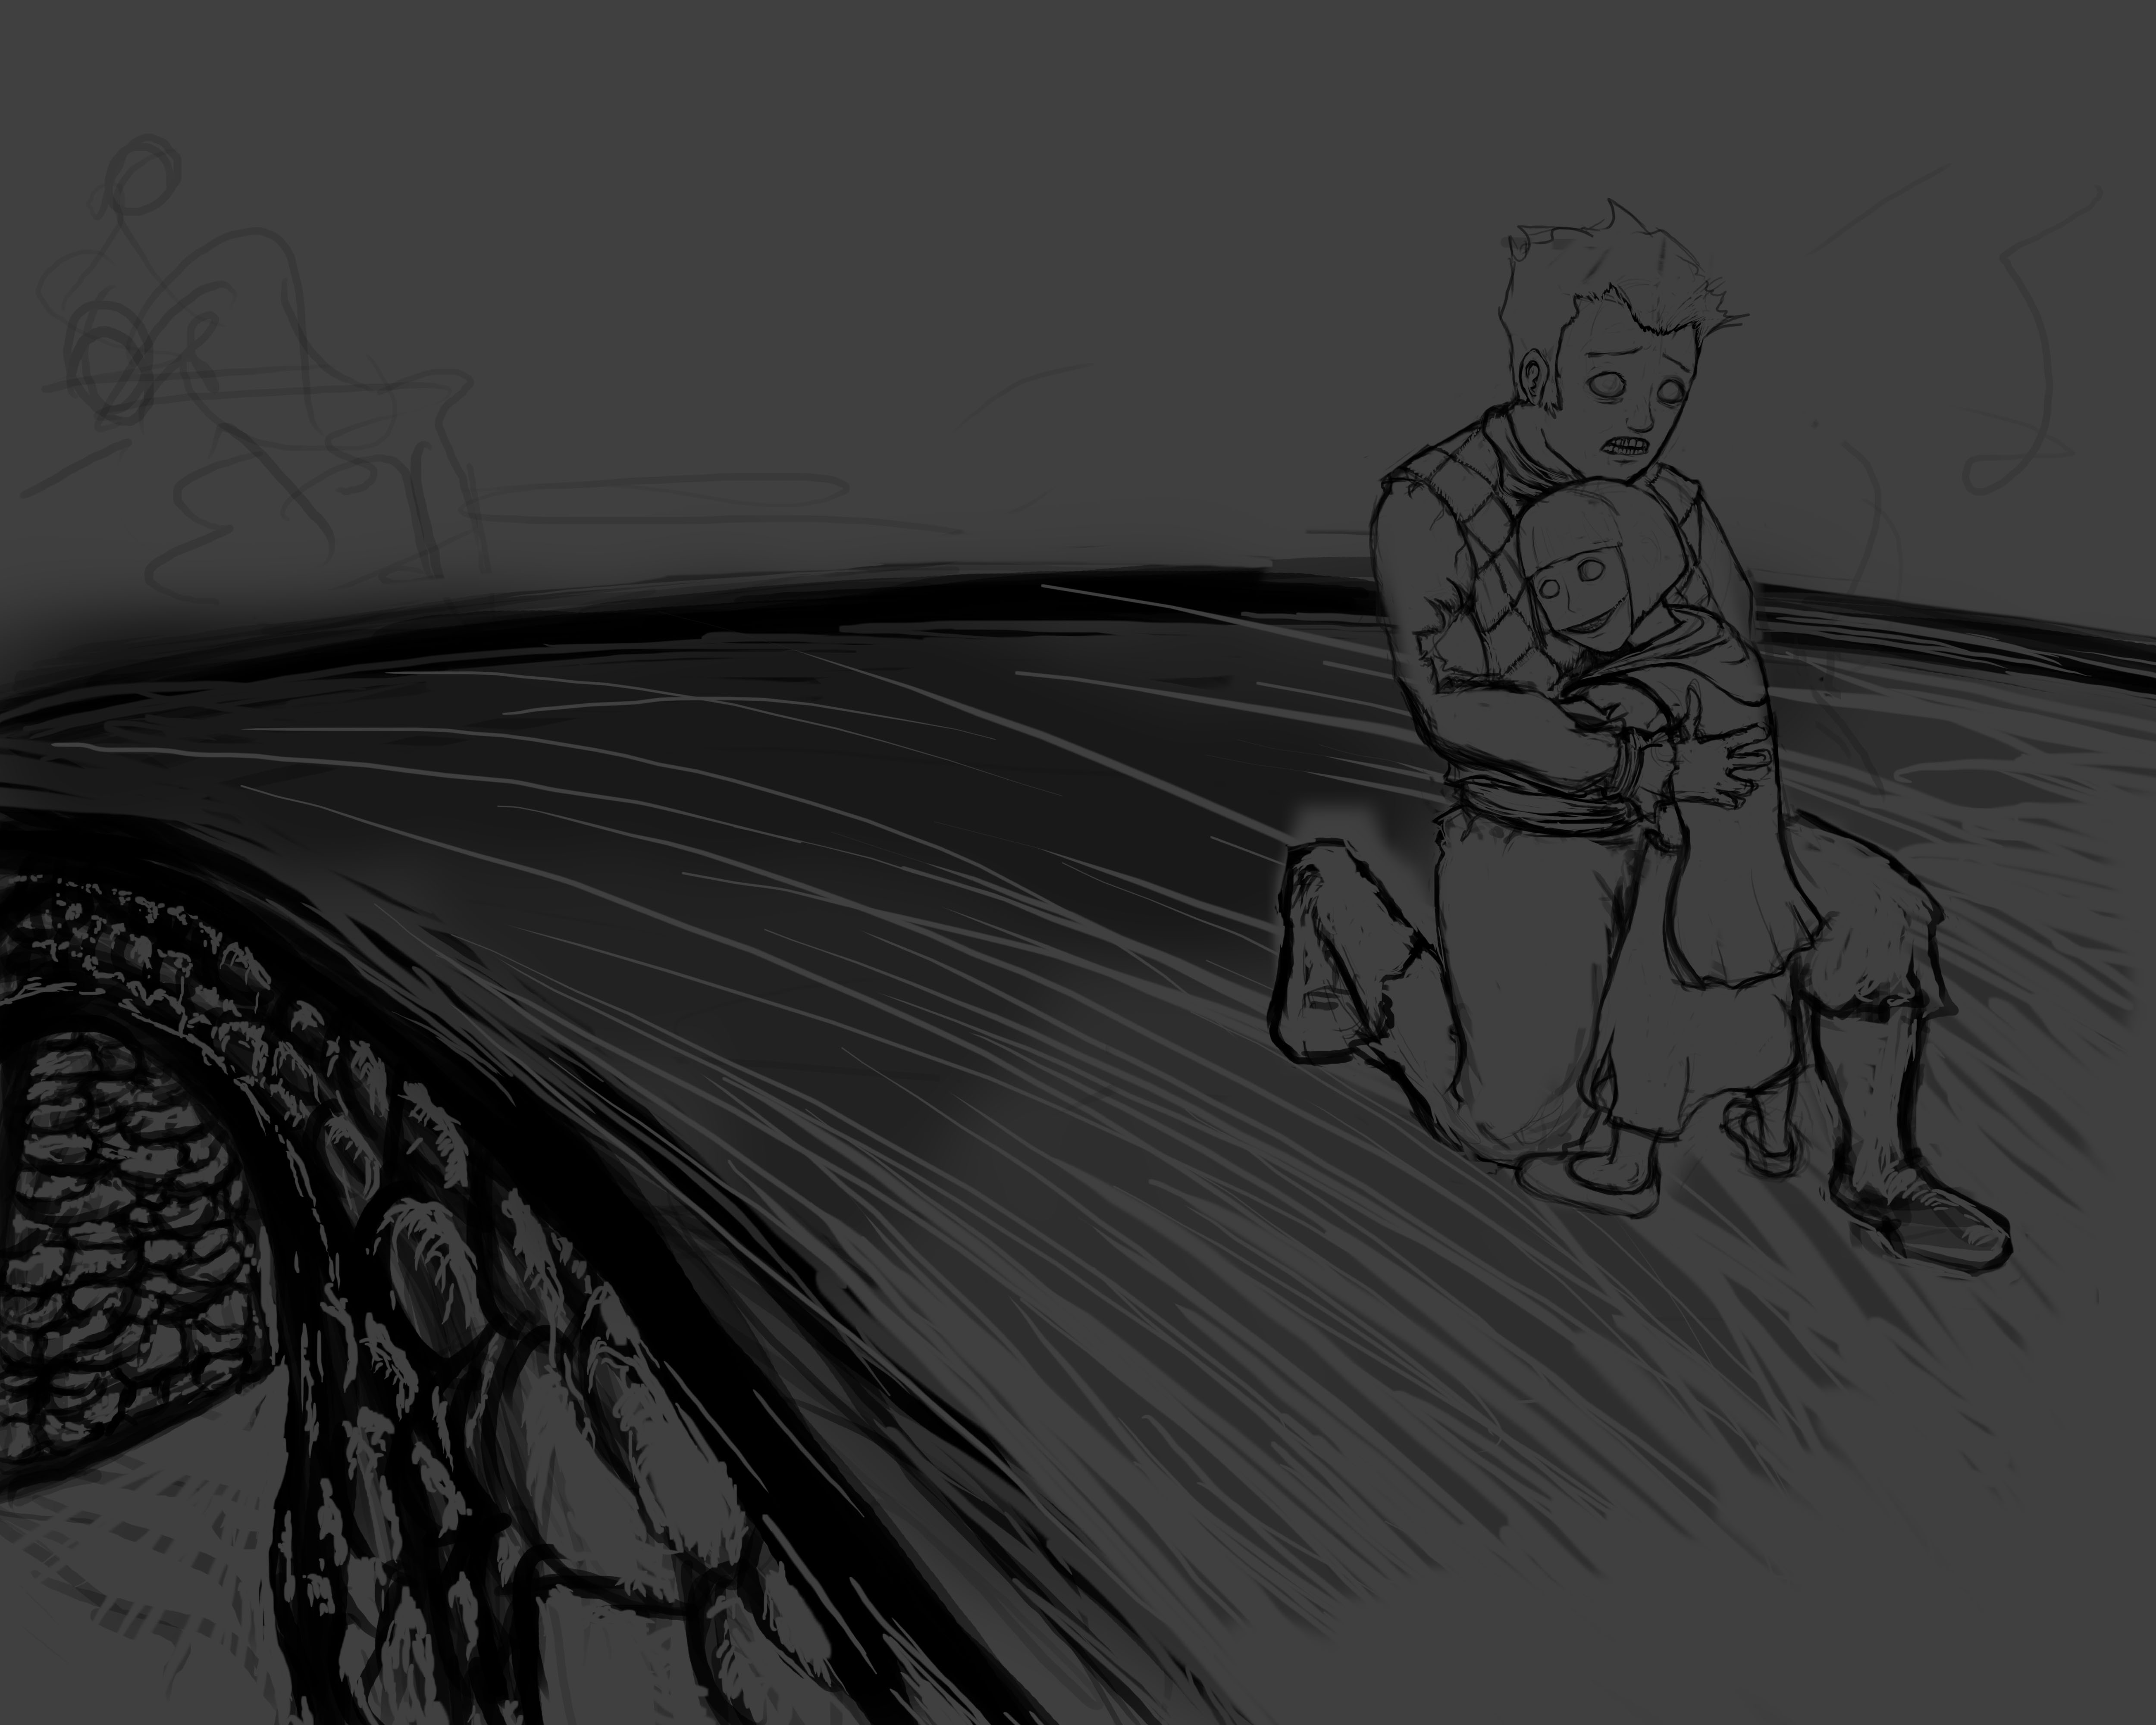
\includegraphics[scale=0.3]{rakaarth4}
%\end{figure}

\begin{picture}(0,0)
        \put(-40,0){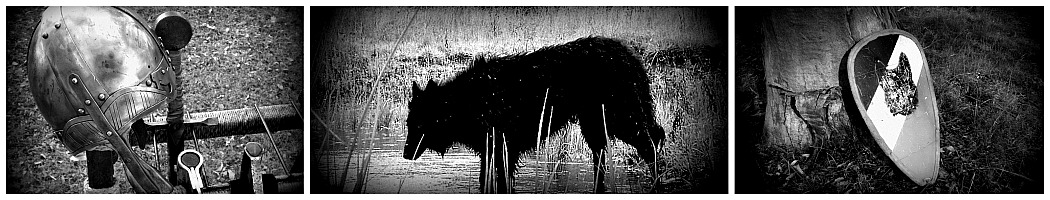
\includegraphics[width=200mm]{Blackwolf}}
        \put(-80,26){
            \parbox[t]{90mm}{
            \begin{flushright}
            \begin{scriptsize}
            \textsf{
            }
            \end{scriptsize}
            \end{flushright}
            }
        }
\end{picture}
\paragraph{World Designers:} oGsMousE, Der Mordenheim
\paragraph{Original Conception:} Der Mordenheim
\paragraph{Assistant Producer:} Ninjacop
\paragraph{Additional Material:} Backstabber, Ninjacop
\paragraph{Editor:} Mother
\paragraph{Art Director:} Der Mordenheim
\paragraph{Lead writer:} oGsMousE
\paragraph{Layout and Typesetting:} oGsMousE and Der Mordenheim
\paragraph{Special Thanks} To Rachel and her family. Lots of love. And to Matty, Jay and Emma, and all other vile things that spawn from London. 

%%%%%%%%%%%%%%%%%%%%%%%%%%%%%%%%%%%%%%%%%%%%%%%%%%%%%%%%%%%%%%%%%%%%%%%%%%%%%%%%%%%%%%%%%%%


%%%%%%%%%%%%%%%%%%%%%%%%%% TABLE OF CONTENTS %%%%%%%%%%%%%%%%%%%%%%%%%%%%%%%%%%%%%%%%%%%%%%%%%%%%


%%%%%%%%%%%%%%%%%%%%%%%%%%%%%%%%%%%%%%%%%%%%%%%%%%%%%%%%%%%%%%%%%%%%%%%%%%%%%%%%%%%%%%%%%%%
\newpage
\pagecolor{gray}\afterpage{\nopagecolor}

%\begin{figure}
%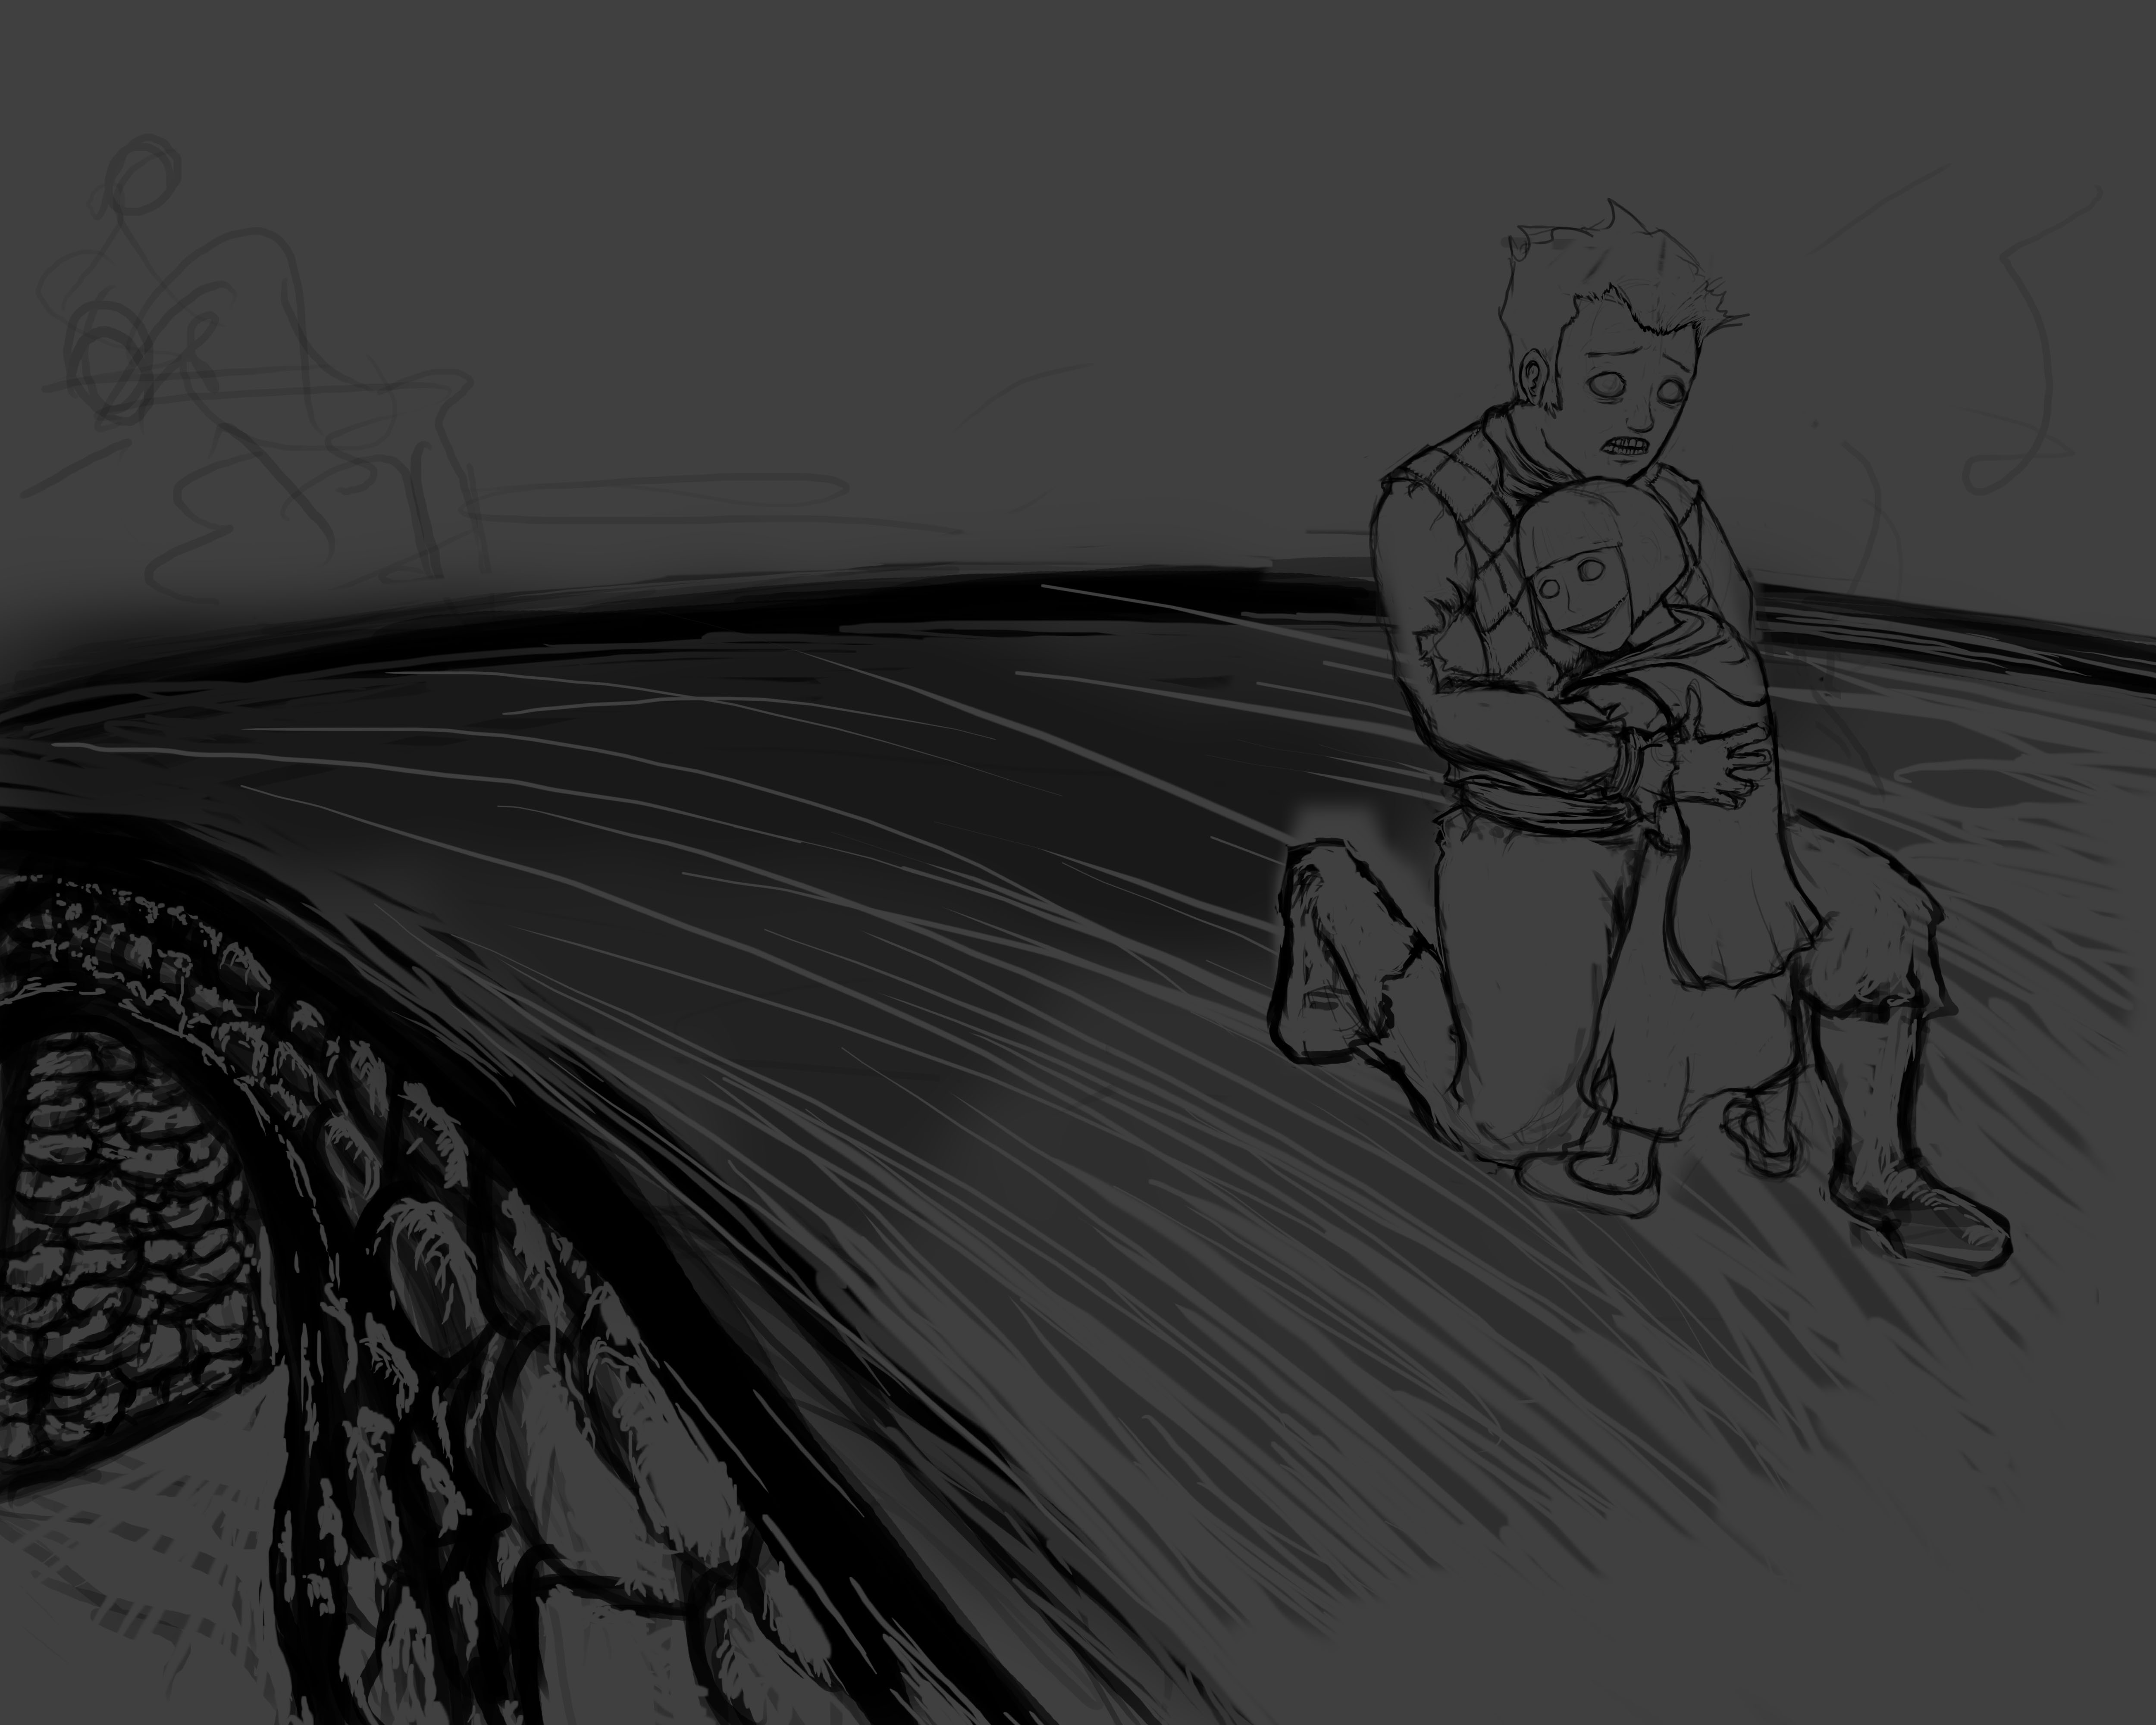
\includegraphics[scale=0.3]{rakaarth4}
%\end{figure}

\begin{picture}(0,0)
        \put(-40,0){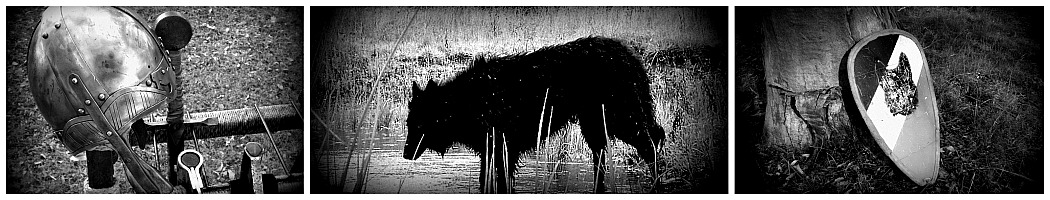
\includegraphics[width=200mm]{Blackwolf}}
        \put(-80,26){
            \parbox[t]{90mm}{
            \begin{flushright}
            \begin{scriptsize}
            \textsf{
            }
            \end{scriptsize}
            \end{flushright}
            }
        }
\end{picture}



\begin{multicols}{2}
\tableofcontents
\end{multicols}


\pagecolor{gray}\afterpage{\nopagecolor}

%%%%%%%%%%%%%%%%%%%%%%%%%%%%%%%%%%%%%%%%%%%%%%%%%%%%%%%%%%%%%%%%%%%%%%%%%%%%%%%%%%%%%%%%%%%


%%%%%%%%%%%%%%%%%%%%%%%%%% THE WORLD MAP %%%%%%%%%%%%%%%%%%%%%%%%%%%%%%%%%%%%%%%%%%%%%%%%%%%%


%%%%%%%%%%%%%%%%%%%%%%%%%%%%%%%%%%%%%%%%%%%%%%%%%%%%%%%%%%%%%%%%%%%%%%%%%%%%%%%%%%%%%%%%%%%

\newpage

%changing the page design temporarily
\changepage{9cm}{9.4cm}{-4.7cm}{-4.7cm}{}{-4.5cm}{}{}{}
%\noindent\rule{\textwidth}{\textheight}
\includegraphics[width=\textwidth,height=\textheight]{haeckelmap}
\newpage

%restoring the standard settings
\changepage{-9cm}{-9.4cm}{4.7cm}{4.7cm}{}{4.5cm}{}{}{}

%\newgeometry{left=0cm,top=0cm,right=0cm}
%
%\maxFrameImage{haeckelmap}
%\pagecolor{gray}\afterpage{\nopagecolor}
%\clearpage
%
%\newpage
%
%%\begin{figure}[!ht]
%% \parbox[t][\mylen]{\textwidth}{%
%% \centering
%% \includegraphics{haeckelmap}
%%
%% \vfill
%% \caption{World Map}
%% }
%%\end{figure}
%
%\restoregeometry

%%%%%%%%%%%%%%%%%%%%%%%%%%%%%%%%%%%%%%%%%%%%%%%%%%%%%%%%%%%%%%%%%%%%%%%%%%%%%%%%%%%%%%%%%%%


%%%%%%%%%%%%%%%%%%%%%%%%%% THE WORLD OF HAECKEL %%%%%%%%%%%%%%%%%%%%%%%%%%%%%%%%%%%%%%%%%%%%%%%%%%%%


%%%%%%%%%%%%%%%%%%%%%%%%%%%%%%%%%%%%%%%%%%%%%%%%%%%%%%%%%%%%%%%%%%%%%%%%%%%%%%%%%%%%%%%%%%%




\mainmatter

\chapter{The World of Haeckel}\label{world}
\pagecolor{gray}\afterpage{\nopagecolor}

%\begin{centering}
% \includegraphics{...}
%\end{centering}

\newpage

\pagecolor{gray}\afterpage{\nopagecolor}
\fontfamily{pzc}
\selectfont
Co-Consul of Ablon enters the Office and the General Autorius sits at his table, golden goblets of wine and a plate full of grapes rests easy in front of him. 

``We had an agreement, that we'd share all revenue.''

``Yes''

``Hereopolis has agreed to give you 20,000 pounds of gold. I want my share.''

``Who told you this?''

``You deny?''

``Who told him.''

``I have spies among his people.''

``If Herod is kind enough to give me a gift, what business is it of yours? A gift is not revenue.''

It is not a gift, it is a bribe. For political and military favours. The cost of which favours shall be born by the state.''

``Peasantry.''

``Let us be realistic. This arrangement of ours can not work if you seek every opportunity to aggrandize yourself at my expense.''

``Laughter. Aggrandize myself. This from the boy whose so called father has been declared a God.''

``An honour he well deserves.''

``You only did it so you might be known as the Son of a God. You have no accomplishments of your own, so you seek to borrow the glory of others.''

``Its true, it was no accomplishment to defeat you at Mutina.''

``You defeated me? You cowardly little shit. You never left your tent. You have never defeated me, in anything.''

``Gentlemen, lets not get overheated. Im sure we can come to some reasonable agreement. I had hoped that you had learnt some humility and discipline. You are still the same old crude, arrogant, lech that you always were.''

``Thats right. Just the same. The same that is still fucking your mother!''
\normalfont

\newpage
\begin{multicols}{2}

Haeckel is a land caught in a perpetual conflict between the common man's reality and the unspeakable horrors of the unknown. It is a home to foul horrors and nightmares made manifest. It's rulers are in constant fear of history relapsing, many feel the doors that lead to the Great War will open once again, spilling atrocities and nightmarish creatures stalking every countryside. To the common people this history is nothing more than an old wives tale meant to keep children in check. Other houses seek to manipulate the knowledge of history to suit their own ambitions. Here deceit is king, whether it be a supernatural horror disguising itself as a beautiful countryside, or the princely noble offering salvation but to a price worth remaining in damnation, or the lowly commoner that is fed lies all his life \ldots

\subsection{How to use this book}
This book provides you everything you need to know to play in the world of Haeckel. Anything that the players should not know immediately will not be described in this book. Each character will not know everything in this book; that is for the player to responsibly decide what he knows.

\begin{framed}\centering
We have chosen to include design commentary as part of this book so that Players and GMs can feast on it and satisfy their curiousity. Anything in this framed box will be that. This is intended to help people get an idea of what to expect in games in Haeckel or for them to enrich their own campaigns.
\end{framed}
%\begin{framed}\centering
% a pantheon of recurring "pseudomythological" entities and a collection of arcane books that supposedly yield insights into the mythology
% \end{framed}
\subsection{Chapter by Chapter} 

\section{Genre}

Haeckel is a vast world. The seven provinces of the old empire together are as large as Western Europe. The vast expanses of North Wall as big as alaska, or maybe even doubly so. It is this size that means that Haeckel defies exact definition. Painted in broad strokes it is possible to make some overall conclusions on its genre. 

Like most RPG settings it can be described as dark fantasy. It has drawn significant influence from literature and media such as REH's Conan, and could even be described as pulp fantasy. But that doesnt really help. For instance, Midgaard is a Kingdom carved in two by political intrigue. Part of it is influenced by Arthurian legend, but with a Gothic Horror type spin that takes it in a new direction. 

In stark contrast, the Megacity State of Ablon draw from the glorious golden age of Rome. Brouliard draws from the Golden Age of the French Chivalric Enlightenment. Culturally its in the renaissance - and often neglected cultural level - and has reached the age of gunpowder.  

Overall it would be fair to say that Haeckel is a milkshake of dark fantasy, pulp fiction, gothic horror with an emphasis on atmosphere, and historical fiction.

\section{The Realm of Haeckel}

\subsection{The Dread Gates} Deep within the impassible mountain range known as North Wall lies the Gate of Ignis, lord of the Flame. When Aratron and Ma’asei imprisoned the other Gods, it is said that Ignis was spared and that his flame was necessary to restore the balance and that another creature, one powerful enough to take to challenge the fire god was imprisoned. Haunting howls and strange lights are reported to emanate in the further reaches of North Wall. Many have attributed these phenomenons to the Gate of Ignis. No one who has ever found it has ever returned, to tell their story.

North Wall is a frontier zone, filled with miners hoping find fortune in the mineral rich mountains, pioneers looking to build a new life, adventurers searching for a rumored lost Kingdom beyond the mountains and those who are looking to hide. North Wall also has its own native secrets hidden within the mountains, giants whom are said to be the children of Ignis, creatures who prey on children who stray too far from their parents, snow like wolves that seem to stalk hunters from unreachable areas, living gems waiting for unfortunate minors to step into their clutches.

In the world of Haeckel there are a total of Seven such Dread Gates. Finding and unlocking their powers are the subject of entire campaigns. Secret Societies in Haeckel are constantly trying to find them and the nature of the Dread Gate's boons is incredibly esoteric. It is said that to unlock them require great sacrifice in the form of a Ritual.

\begin{figure}[h]
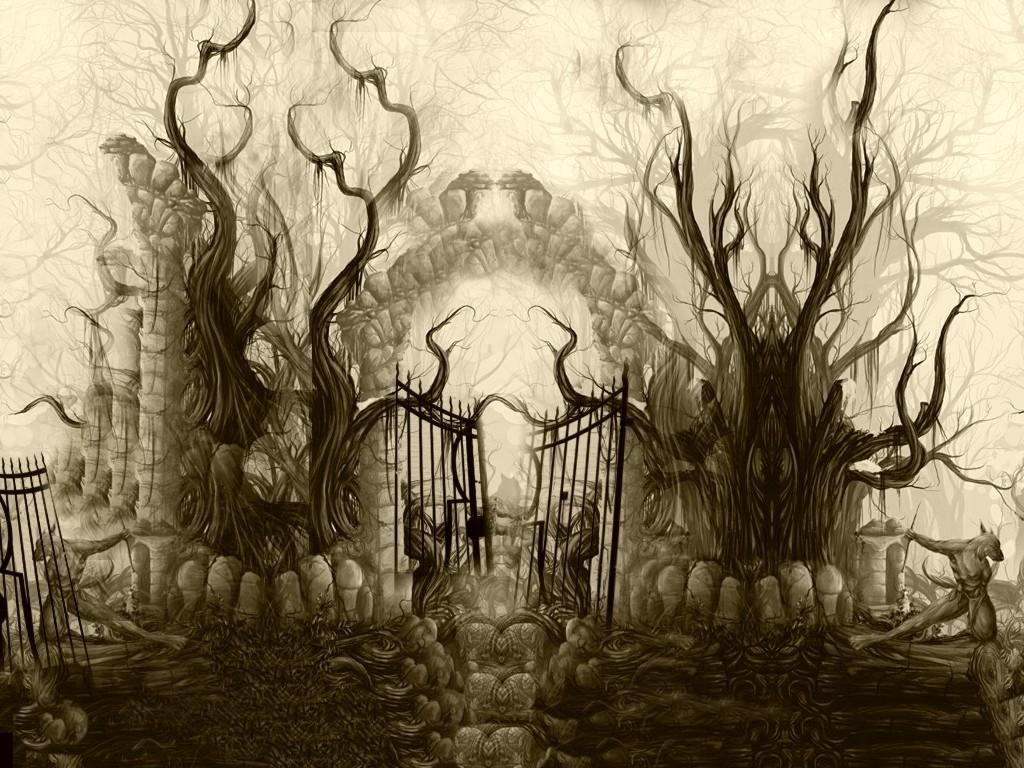
\includegraphics[width=\columnwidth]{gates-of-hell-open}
\end{figure}

\subsection{The Powers That Be} Power exists where people believe it exists. It is both fickle, complex, and its ramifications are terrifying. The World of Haeckel has both overt and covert powers that shape its very existence; past, present, and future. 

\subsection{The Invisible War} Since Antiquity the Mages of Haeckel have been in perpetual war with each other from behind the scenes. The 1000 years of bloodshed have stained the land. The Nobles and Powers That Be whom dominate the world have ensured that the details of this conflict remain in secret. To the common man the Invisible War is a shadowy myth that is best ignored. The reality of this War is simple. In Haeckel, the cost of developing arcane research is immense. In a bygone era, some Mages sought to channel the wealth of nations in order to fund it. They are an extremely secretive lot and they often use advanced techniques to ensure that no other Mage can acquire their secrets. In financial terms, the cheapest way for a Mage to gain new power is for him to slay another Mage and steal their knowledge. Thus, every Mage is compelled by the nature of their work to hide in the shadows and avoid drawing attention to themselves lest they be preyed upon by other more dangerous individuals. This however has some extra complexity. You see, the most powerful mages are not interested in the small fish mages. They want them to grow in power, so that one day they may take their work for themselves. At the same time, some Mages realise that very complex tactics has evolved from this conflict. Weaker mages are often used as bait by more powerful Mages in order to ambush other powerful predator Mages. Thus you have this complex game of cat and mouse. 

\paragraph{The esoteric nature of Magic} In most Player's Handbook type products there exists a sizable chapter on spells that exist within the game. We have chosen to explicitely omit this from here. In Haeckel RPG magic spells are a source of mystery, wonder, and an integral part of the joys of discovery for players. Simply put, it is an overt declaration that the players will not know what to expect with regards to magic. That is fundamental to its esoteric nature. Even the way that magic works is unknown initially. There are a number of Magical Theories, some work, and some dont - and puzzilingly some that work might even contradict each other working systems. 


\section{History}

\begin{tabular}{l|r}
    \hline
    Year & Event \\
    \hline
    0    & The First Apocalypse \\
    350 & The Invisible War Begins \\
    950 & The Time of Summer \\
    1250 & The Great Catastrophe \\
    1251 & The Great War \\
    xxx & The Hour of the Knife \\
    1350 & Current Day \\
\end{tabular}


The study of Haeckel's past can prove to be a maddening exercise. The denizens of Haeckel have rich cultures and histories dating back centuries. Some of it is mythical and some of it grounded in fact - albeit interpreted by the Powers That Be to suit their own needs. Through a long tradition, and a shared history, the provinces of Haeckel have adopted the Haeckelian calendar to mark the passing of years. Isolated areas however may track time through their own reckoning. 

\subsection{The Time Before}

The true origins of Haeckel remain a mystery. Gypsy,  Elven, and Dwarven legends, as well as numerous creation myths suggest that the current inhabitants are descendents of a terrible race from a Land Beyond whom migrated to Haeckel. Though at times contradictory, common themes hint that the continent may have existed for eons, forever ebbing and flowing in an eternal cycle of expansion and decay. 

\subsection{The Long Summer} 

\subsection{The Fall} Janus Thurinus blessed King of Haeckel, unifier of Seven Territories, Keeper of Justice and Bridge between the Elven and Man. Under his rule Haeckel thrived in an era of peace and prosperity. This era is also known as the Time of Summer, for The Fall that was to proceed.
In the final years of Janus Thurinus' reign, incompetent eunuchs deceived the queen and persecute good officials, and the government becomes extremely corrupt on all levels. The elites of society allowed degradation to occur, using the political chaos as a shroud to mask their illegal occult practices. A rebellion breaks out lead by the perpetrator of the chaos Wiglaf Lysander, High Constable of Haeckel’s Royal Guard. The rebellion is barely suppressed by the troops under the command of Gestae Ni, Vice Captain of the Royal Guards. Meanwhile Imperial Wizard and Queen's Advisor, Luoyang Xi, attempts to halt a growing cult within the ruling nobels known as The Phex. Louyang uncovers a plot to open up a legendary Dread Gate, ignored by the Queen who is fighting to save her kingdom and repair harm caused by the rebellion, Louyang Xi decides to confront the cult. He interrupts their ritual causing a catastrophic chain of events leading to the destruction of the capital, ultimately shattering the Kingdom of Haeckel and cursing its land. This event has been dubbed the Great Catastrophe. A great quake splitting a region of Brouilard in two, opening a great chasm known as The Scar of Rock Rose, weather takes a more magical property causing strange toxic storms which scorch the land, strange plagues that seem to have an intelligence of their own mutating its victims. Horrors that were once fables made manifest stalk the realm. Haeckel’s days of Summer now a fading memory.

Though devastated and torn the rebellion continues and many of its culprits survive The Great Catastrophe. After the dust settles the young Prince Aglar is found by soldiers of Wiglaf Lysander, who proceeds to seize control of the imperial capital under the pretext of protecting the Prince. Wiglaf Lysander also initiates a murderous campaign to recover Imperial relics lost due to Great Catastrophe. Imperial chancellor Ozymandius escapes and issues an imperial edict in the Queen's name to all regional warlords and governors, calling them to rise up against Wiglaf. Under Gestae Ni's leadership, [[[wiki:the-eighteen-warlords | eighteen warlords and mercenary companies form a coalition force in a campaign against Wiglaf, but undermined by poor leadership and conflict of interest, they only manage to drive Wiglaf from the capital to the ruins of Midgaard. Wiglaf is eventually killed by a mercenary in dispute over a lost Royal Relic. Alisuim of Yares, healer and matriarch to a militia of medics and priests finds the Imperial Seal and keeps it secretly for herself, further weakening royal authority. Without a strong central government, warlords begin to rise and fight each other for land, plunging Haeckel into a state of anarchy. Mysteriously once dissolved noble House, Mordenheim, has rekindled and has reported to be lead by Wiglaf's assassin, the former mercenary captain; now, Dracs von Mordenheim. Dracs von Mordenheim then established the mysterious Order of the Grim Shadow and rallied a small army to battle his former employer Ba'al Xebub, sovereign Merchant King of Abyssal. Remnants of the Lysander family have waged a blood feud against the Mordenheims.

\subsection{The Great War} The Great War spanned a generation. The Great War was one of attrition, such the magnitude that most of Haeckel may never recover from. Lands stripped of resources to produce terrifying war machines, towns and villages depopulated forcing all able bodied person to fight for either side. Lysander’s blood feud depleting the Wiglaf family tree, forcing The Dark to make unholy pacts with the dark coven of The Phex. Soldiers fleeing from encounters with The Dark report seeing their generals transforming into horrifying unkillable man-beasts. The forces of Ba’al Xebub also suffered heavy losses, with income depleted Ba’al forced to sell of his treasury piece by piece to fund his vast mercenary army. Rumors amongst Abyssimiar and Ubris Furor tell the story of Minotaurs visiting towns, villages and desert camps to force the populace in to slave armies. The Order of The Grim Shadow too suffered heavy losses, perhaps the heaviest being their leader’s loss of humanity. The once loved leader became more and more reclusive. Rumors throughout western Haeckel tell tales of House Mordenheim experimenting in the forbidden art of Necromancy to create an army that could never deplete. Other and perhaps more troubling reports tell of the members of House Mordenheim being monsters who Bleed of Shadows.

Unbeknownst to The Dark, Prince Aglar was spirited away at the start of the Great War by Alisuim. Protected and groomed to bring forth a new era of peace and reunify Haeckel, Prince Aglar rallies the remaining allies to the fallen throne and enters the melee as The Principality of Thurinus. With the combined might of those whom view the Principality with an almost religious zealous they emerge victorious battle after battle, even halting the march of The Order of The Grim Shadow’s undead army.

The juggernaut that was The Great War is slowly coming to a halt. Due to successful sabotage attempts to all other factions The Principality’s goals are well within reach. Ba’al Xebub’s forces now feeble and non existant, many mercenary companies revert into banditry, Minotaurs abandoning their former master on a quest to reestablish their ancient homelands. The family of the Dark, despite having bestowed unholy blessings becomes almost extinct. The power over the undead horde ebbs and fades leaving only the members of House Mordenheim as The Order’s military might.
Yet despite The Principality’s military quickly regaining control of Haeckel, Dracs still pushes on his quest for revenge. With only four members of House Mordenheim, The Order of the Grim Shadow manages to slaughter all but one member of Wiglaf’s lineage; leaving the sole survivor to lament over his families short comings. He then encounters Prince Aglar with his closest ally House Liebentod within Ba’al’s Obsidian Spire within Abyssimiar. A battle ensues, and none seemed the victor. Despite the strange and perhaps unholy nature of the members of House Mordenheim they could not slay these zealots. Recognizing the passion within his opposition to that of his own Dracs surrendered, only on the condition that he alone may finish his ascend to the top of the spire so that he may meet Ba’al face to face.

Before facing Ba’al, Dracs faced his former general comrades, all whom too weary to continue the war. Nothing is known of the meeting between the two, only that Dracs descended the tower and that no one has ever sighted Ba’al again. From the meeting between the two forces, House Liebentod defected from the Principality to join that of The Order of The Grim Shadow. This caused a brief tension between the two remaining forces and caused rifts to open within the Principality, some members rallying for the destruction of the Order, while others expect House Liebentod to pacify The Order of The Grim Shadow. Within a week Dracs himself met with the Prince and swore fealty to the throne and assisted Prince Aglar using The Order of The Grim Shadow to aid his quest in unification. Prince Aglar in turn recognized House Mordenheim as a legitimate noble house of the highest regard. Despite bringing a degree peace to Haeckel this action formed a permanent divide within the Principality. Those who remained distrustful of House Mordenheim, distant themselves from the Prince, silently plotting the demise of House Mordenheim, some even plotting the demise of Prince Aglar.

\subsection{The Hour of the Knife} The Great War had officially ended, and although The Principality of Thurinus had won the war, their ultimate goal of peace and unification was lost. Noble houses became more and more distrustful of one another, the leaders of several houses turn missing or have been reported to have been assassinated. Veterans of the war roamed the land scavenging a looting all that they can. Once enslaved creatures used to terrorize enemies now left unchecked and prey upon helpless villagers. The Great Houses of Ablon who stayed neutral during the Great War, since then Ablon has become increasingly distant instituting an isolationist policy. Due to the magical horrors that were unleashed upon the world a number of veterans from all factions have banded together to form an organization, calling themselves The Puritans; these men and women have vowed to cleanse Haeckel of all magic. A group of mercenaries have found new methods to survive during a time of peace, now hiring themselves to that of common man as a means to enforce justice; The Company is called The Enkertons. The survivors of The Dark, left torn and broken have found ways to survive Ignis, the sole survivor of the Wiglaf lineage, slowly rebuilds his family. As new factions form many old ones meet violent ends. A string of assassinations stretch over Haeckel, the mysterious group known as The Phex becomes more active as knowledge of The Dread Gates scattered across the land slowly become more available to those who seek them.

Dracs von Mordenheim is reported have met his demise on the end of an assassin’s blade, the suspected culprit a sleeper agent of The Phex. Shortly after the death of Dracs, his sworn ally the Prince Aglar disappears, his fate unknown. He leaves the Principality with twin sons whom grow up to hold different views on how Haeckel should be protected. In the wake of the war a total of 24 Houses suffered mysterious fates, some never recovering after the death of their liege lord. It is unknown whether all of these deaths and disappearances are due to some Phexian plot.

\subsection{The Present} 

\section{The Geography of Haeckel}

Depending on ones outlook the inhabitents of Haeckel call it by different names. Like the chest of a sleeping beast the world of Haeckel expands and contracts according to the needs of the Dictators whom rule it. Cartography, the art of mapping, is a lost art. Some live a claustrophobic existence; living and dieing for their entire lives within 20 miles from their place of birth. Some others with more intimate understandings of the land greedily hoard these secrets for it is a key advantage to attaining wealth. 

Untold millions of Humans exist in Haeckel. Their lives are brief, flickering lights, trapped in drudging poverty as farmers whom cultivate the land. Hundreds of small cities dot the land. Towns and villages are innumerable, to map it would be futile. While this may seem really dense, the reality is that only cities are a dense mass of bodies all compressed together like sardines in a small area. Haeckel mirrors Western Europe in geographical area and is actually quite depopulated. Land, and thus grain output, is the ultimate measure of wealth for any landed nobility; though, multiple schools of thought exist on the nature of power in Haeckel.

Haeckel can be thought of as having Seven Kingdoms, each with a united history that loosely ties it together as they lived together before the Fall under the vast shadow of the Empire with its center in Avalonia. To the north of the old Imperial states is North Wall. It is the howling abyss of the world, a land of unimaginable size with a breadth that cannot be measured. To the south is the independent Kingdom of Abyssimiar. To the native Haeckelians, Abyssimiar is an exotic realm that is both eerie and terrifying due to its alien culture. Abyssimiar managed to stay independent by virtue of its powerful navy and extremely harsh deserts that contributed to its geo-political isolation. Even further south is the Southern Continent, the realm of the Unknown. It is virtually cut off from the rest of Haeckel but its creeping influence grows year by year like worms in shit.

\begin{framed}\centering
Part of the appeal of exploratory game design is learning the world and getting map awareness is a key part of the game. Going from a scared little guy with no idea whats in the world to a hardened adventurer able to navigate his way through the entire world with little sweat. 

To this end, significant thought has been put into promoting exploration in the game mechanics. This is both exploration in the sense that you travel around and in the sense that you be creative with the in-game content. For example, the Alchemy and Herbalism systems promote exploration since you must find ingredients and experiment with them to see what happens. It is one of the design mantras that we have aspired to.
\end{framed}

% Petty jealousies give birth to considerable envy.  
% Law of the Minimum
% A Legend, a Prophecy, that their Leader will come from a foreign land and guide them to true Freedom. The people here are simple and survive on hope. 

% Government claims are not tantamount to the truth


\definecolor{shadecolor}{gray}{0.9}
%\begin{shaded} text \end{shaded}

\begin{snugshade} "I live solely for myself, and there is no end to it, as long as there are people to kill in this world I will never disappear." -- Ordrelan \end{snugshade}


% Maxims of Madness
% Tenets of Terror
% Doctrines of Damnation
% Creed of ...
% Fundamentals of Fear
\paragraph{Exploration \& Campaign Play} 

%   
 
% Exploration is promoted
% Non-linear gameplay.
% Complete the dungeons in any order that you want.
% The game is full of secrets that promote exploration. There is no artificial limits stopping you from doing certain things. If you get something, you can play with it. 
% Learning the world and getting map awareness is a key part of the game.
% Take any road you want. Bends over backwards to reward and reinforce exploration. The only way to learn about the world is to explore. You may end up wandering the world and getting your butt handed to you, but thats fine. 
% It minimises the risk of dieing and frustration from it by speeding up the character creation system so you can rapidly get back into the game. If you die, and lose some loot, you could try find it again with a new character.
% Its upto the players to find landmarks and make note of them.
% Go from a scared little guy with no idea whats in the world to a a hardened adventurer able to navigate his way through the entire world with little sweat. 

% Choosing paying taxes or not
% Items
% No challenge system to balance encounters against the players. Its upto the players to decide if they're capable enough to deal with a situation
% Learning how capable you are is part of the exploration of the game
% 
% % Brazier
% % Potted Plant
% % Fountain

\paragraph{Political Intrigue} The Kingdoms of the Old Empire compete viciously on the nation state stage. And within those Kingdoms cutt throat politics and scandal is rife as the various power players thirst for an even greater slice of the pie. Political intrigue is one of the most common overrarching themes to the narrative in Haeckelian campaigns. Also, a significant proportion of the system is built so that the players may immerse themselves in it.

\begin{snugshade} "And so it begins. The trap is set. Centuries of humiliation visited upon my family will be avenged. Their plan is elegant and vicious. At the moment of his greatest confidence, traitor strikes. Pervading common wisdom is the mark of every great conspiracy. Even though they would never admit it, a popular man always has many who want to get rid of him. Our House will be more powerful than ever. Alone and vulnerable at the edge of society, we will make them come face to face with fear. We will make them turn on each other like rats in a flood." -- Raakarth \end{snugshade}

\paragraph{Discovery and Exploration} A key component of Haeckel that distinguishes it from other RPG settings is the concept that the vast majority of the content needs to be discovered in the game and thus are GM secrets. There will be an entire Herbalism and Alchemy subsystems, for example, built for such a purpose among many other things. 

Therefore the purpose of this book is to help the players build characters that fit within the setting and are provided enough ammunition to build powerfully evocative characters that they could then breath life into in new and interesting ways. 

\paragraph{Character Gameplay} We aimed to promote ways such that different character types have a genuinely different gameplay feel. There would be different routes through the gameplay world, in which different obstacles are faced, and different tactical options for various situations. This idea has influenced our module design where we promote replayability. 
 
\paragraph{Craftsmanship} 


%\subsection{Themes}
%
%When we set about creating a setting with some roots in pulp fiction we immediately thought of Lovecraft and the repeating themes used in his works. Typically they would revolve around ignorance vs knowledge and the standard norms of society being shaken by something foreign. Dracs' imagination drifted towards more modern medias. Italian exploitation horror (grind-house films, as some have dubbed) - which I would consider to be the modern film equivalent to pulp fantasy fiction and 80's horror films. 
%
%\paragraph{Ignorance vs Knowledge}
%\paragraph{Pandora's Box}
%
%\subsection{Current History}
%Roughly one hundred years ago a supernatural apocalypse and brutal civil war occurred that rocked the continent. The Old Empire had fallen, and each of the seven provinces of the Empire now act as independent states. A number of other regions existed as independent states outside of the Empire. The tragedies and bitter conflicts of the past still scar the land. History has not been forgotten and sets the tone for the present. 
%
%The seven ex-imperial provinces are: Ablon, Avalonia, Brouliard, Midgaard, Nes, Nosquam and Ubris Furor. 
%
%The foreign provinces are: Abyssimiar, North Wall, Grul, and the Southern Continent.

%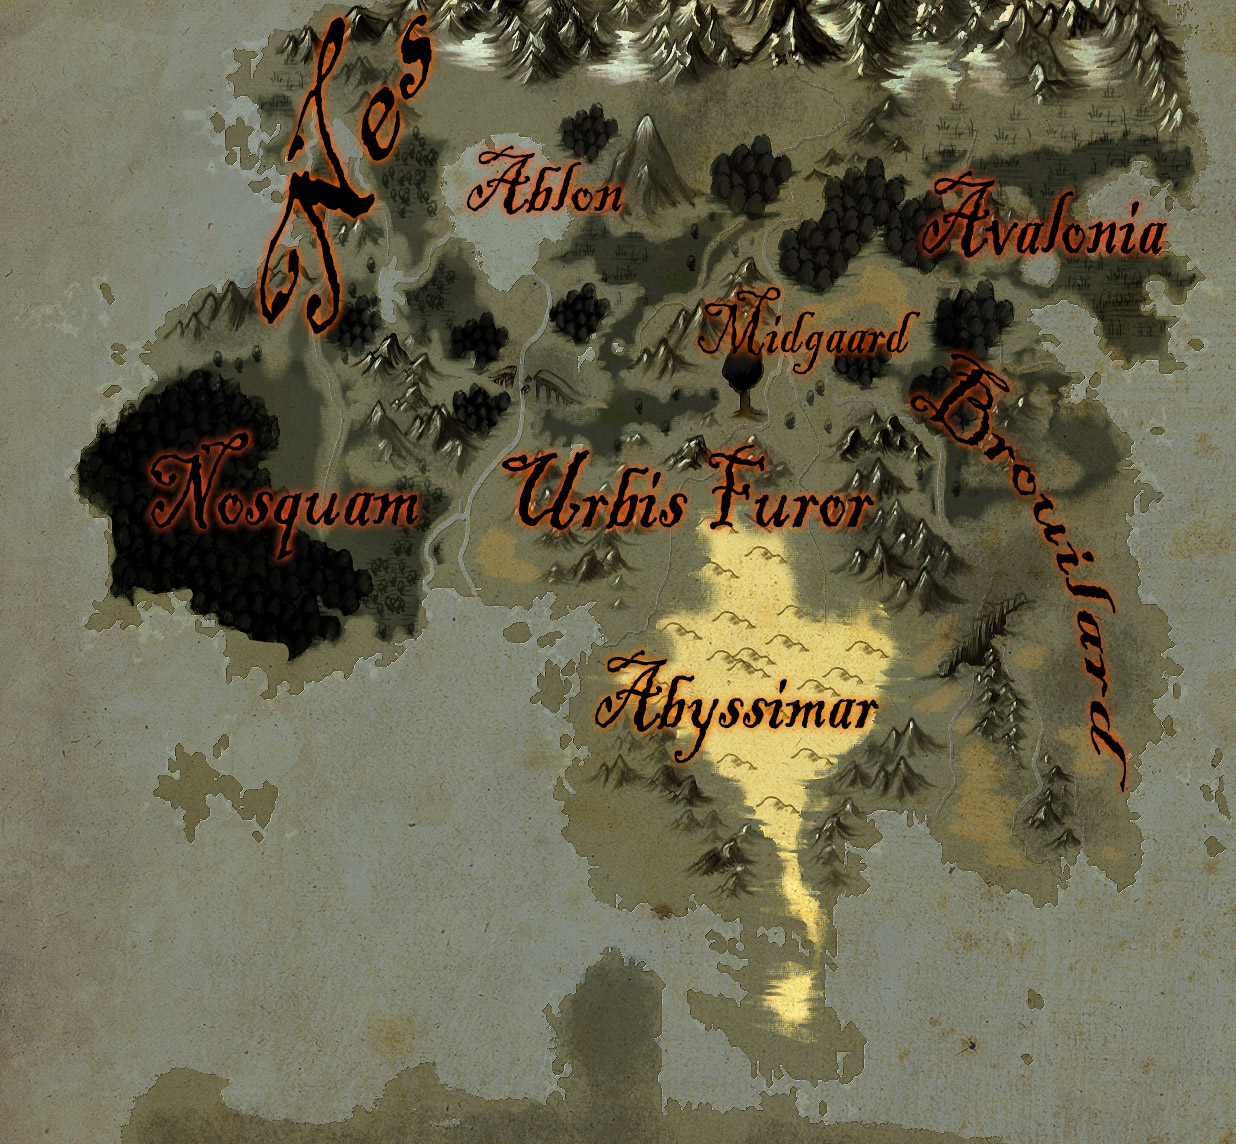
\includegraphics[height=\textheight, width=\textwidth]{Haeckelmap.jpg}
        
%\ThisCenterWallPaper{1}{Haeckelmap.jpg}

\subsection{Ablon} 

The incomprehensibly vast Mega City of Ablon casts a tremendous shadow over the world. Its influence is far-reaching and its achievements are prodigious and monumental. Three great Houses rule Ablon with ironfists, their powers are sweeping and their desire to see each other's downfall is boundless. Tales of their ambitions are widely known and it is said that they seek to make the Mega City State into an Empire in its own right. Many other smaller cities exist within the greedy aegis of Ablon, all are puppets that's sole purpose is to provide grain to the capital of this region. The decadence, wealth, and architecture of Ablon is lofty and unforgettable as it sets the standard for all of Humanity.  

Naming Scheme: Roman and Greek

\subsection{Avalonia} 

The Old Capital. Wasteland of the Old Empire and the most valuable province in the known world. Because it is here and only here where magic is found in its most raw form. Without the phex, there would be no Powers That Be. The greatest treasure in the known world. It is here where the only opened Dread Gate exists. The Mages that control it control the destiny of the Old Empire. But despite this, it is locked in a never ending struggle to survive against supernatural horrors. Those few survivors that stubbornly remain do so at a terrible cost as they must survive without the protection of civilisation in a stone age existence.

Naming Scheme: Arthurian and Latin

Avalonia is a province that is drenched in horrific myth and legend. Vast amounts of misinformation exists outside of this land. Mundane characters would likewise be trapped in this maelstrom of misinformation. Avalonia is a land where the unreality is breaching reality. Only Mages would have even a modicum of understanding about the true natures of this realm. 
\begin{figure}[h]
\includegraphics[width=\columnwidth]{avalonia4}
\end{figure}

%\begin{multicols}{2}
\subsection{Brouliard} 

Filled with every kind of social insect, Brouliard is a grand masquerade teetering on disaster. The cities have embraced the ideals of the Enlightenment and reached a Golden Age of Prosperity under the absolute rule of Queen Sophia. Brouliard is now the cultural diamond of the known world but it still wrestles endlessly with its barbaric past.

Brouliard society is a tangled web of competing forces. Brouliard civilisation rests on a political tripod; the most unstable of structures. A deceptive balance of power exists between the Absolute Queen Sophia, the Other Society and powerful Merchant Houses. It is complicated by a feudal trading culture and a political past of absolute tyranny. 

Naming Scheme: French, Greek, and Early Germanic

% width=0.5\textwidth, height=0.5\textheight

%\end{multicols}
% The cultural diamond of Haeckel. Queen Sophia has produced a Golden Age of prosperity for her people. This land is based of Renaissance and Chivalric France as well as 18th century Russia. Its a land that is progressing towards the Enlightenment but paradoxically the benevolent ruler Queen Sophia is also an Absolute Monarch and a Tyrant. 

% Be sure he recalls his flimsy denials before the face of death's sweet smile. 

% Better to miss an opportunity than invite disaster
% My people are cautious and pragmatic.


\subsection{Midgaard} 

Midgaard is a realm both glorious and terrible. It is a grand tapestry of gothic medieval horror. Within this blood drenched kingdom, life is countlessly born, and unceasingly ended in almost cyclical conflict. The Lords of this land are doomed souls tarnished forever by the sins of ambition, pride, honour, and glory. The battle against evil can be daunting - even terrifying - but not futile. Most stew hopelessly, drunk on their desires, but those special few are martyrs who end up choosing death over damnation.

The people of Midgaard are fearful, fanatical, and violent lot. Alone, peasants are weak and cowardly. But as a mob they can quickly become vicious like a bloodthirsty pack of wolves. The chorus of baying peasants as they burn a witch is to be seen. Civilisation is not safe as it once was; savage bands of bandits roam the countryside that attack, murder, and pillage unprovoked, using speed and shock tactics to stay alive.

In Midgaard, the unnatural is accentuated by emphasising the natural. For every prowling night terror, remember the village of decent folk it preys upon. For every tale of obsession and betrayal, consider the families whose loving ties see them through the years. In this Kingdom there is a distinct contrast between wondrous and wrong.

Naming Scheme: Arthurian, Middle English, Babylonian

% The land of Gothic Horror, Medieval Fantasy, and Arthurian legends. This land has an English and French medieval theme that aims to bring to life the tales of terror of those tragic times but at the same time bring to light pleasing aspects of medieval rule. Evokes a shivering symphony of horrors and splendid tales of tragic heroes teetering on disaster. 

\subsection{Nes} 

Descendants of an ancient naval Empire that is said to pre-date Haeckel itself. The people of this land cling to the Old Ways; they are a cautious and pragmatic people whom have the saying: better to miss an opportunity than invite disaster. 

The remnants of their civilisation is a flickering light among the darkness. The land is haunted by the tragedies of its past that are now made manifest in reality in the form of a parasitic menace that curses this land. It is known as the Phantasmal Forest; it is made of plant lifeforms that can infect any organic matter. It unceasingly spreads and the native Nessians wage a perpetual war against it to halt its progress. 

Long and bleak periods of civil war has crippled the Kingdom. Savage bands of bandits roam the countryside; many of which are traitors whom had pledged their service to disenfranchised nobles who lost the Blood War. 

The foreign Midgaardian Church stubbornly grasps for power in this land. They are establishing monasteries behind thick stone walls throughout. Their scribes create beautiful illuminated manuscripts, embellishing ancient knowledge and religious thought. Those monasteries ring with newly invented choral harmonies.

The ruler of this realm, Jarl Holgerholm V, aims to rebuild his Kingdom and return it to its former glory spoken off in legend. He faces massive obstacles for his Kingdom is entombed in a dark age and escape from this terrible cultural decline seems impossible. The end of his Kingdom looms menacingly on the horizon. But he is a strong King, one whose true education lies in armed military campaigning. 

Naming Scheme: Norse, Saxon, and Celtic

\begin{figure}[t]
    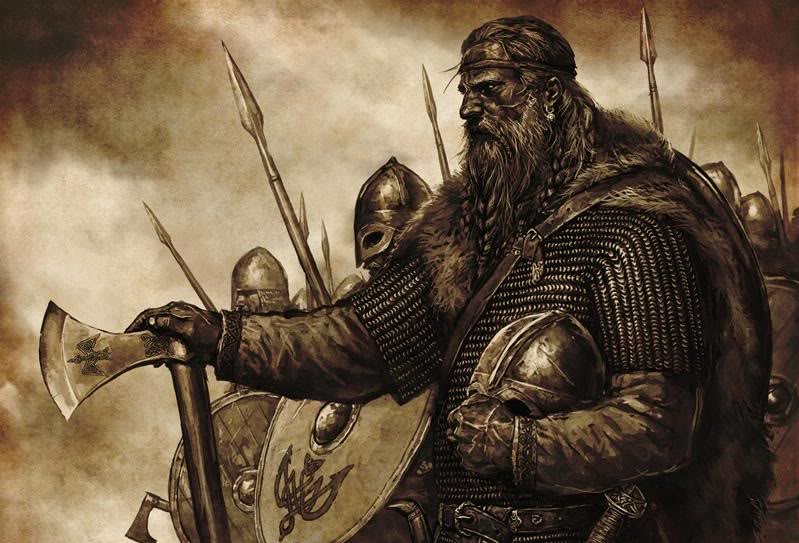
\includegraphics[width=\columnwidth]{viking1}
\end{figure}

\paragraph{Nosquam}

Naming Scheme: Latin, Any

\subsection{Ubris Furor}

Naming Scheme: Persian, Hebrew, Arabic, and Mongolian

% Between the lines of my journals is the struggle with Humankind's view of itself. The motives of our darkest past wells up and with which we must not only live but also contend. The land is haunted by the tragedies of its past made manifest in a parasitic curse that terrorises the land. 

%\paragraph{Nes} What you have here is a Viking themed Death World. The entire land is menaced by a terrible phantasmal parasite that infects any living organism. Over one third of the Kingdom is infected in a colossal biome known as the Phantasmal Forest. To survive, the people here have adapted to become some of the hardest motherfuckers to have ever lived, but at a great cost. Forget the advancement of culture, of science, and of common understanding. They are trapped in a dark age of perpetual war. The goal of every man, woman, and child, is to survive and keep the human race alive. 

\section{Culture}
Culture is an immensely important and often ignored most of most RPGs, and there is a tendency for most of them to be "generic medieval". I describe them as such because they tend not to actually capture the glory of the medieval period, its tragedies and culture of treachery. 

There is a great disparity in the cultural advancement of the provinces in Haeckel. Additionally, while a particular region could be of a certain culture level, it is entirely possible that the outskirts are more savage - as is especially the case with Brouliard where it has embraced the Renaissance in the cities but is still trapped in the Late Medieval Age in its vast farmlands. 

Thus I have created a Culture Level system that gives a general idea of the level of development. It also helps drive home to the players and GMs the impactful differences between the cultures - and so for this reason I see it as invaluable. 

\paragraph{CL 0 - Savage}

\paragraph{CL 1 - Stone Age}

\paragraph{CL 2 - Bronze Age}

\paragraph{CL 3 - Iron Age}

\paragraph{CL 4 - Classical}

\paragraph{CL 5 - Dark Age}

\paragraph{CL 6 - Early Medieval} 

\paragraph{CL 7 - Medieval}

\paragraph{CL 8 - Chivalric}

\paragraph{CL 9 - Renaissance}

Avalonia is completely crippled and is literally in the stone age. Nes is perpetually trapped in the dark age due to its own troubles. One of the aims of Haeckel was to provide rich cultures that have impact on the players. 

There is no "generic medieval" here. The Medieval realm of Midgaard really drives home what Medieval means, in every sense, good and bad. North Wall is the howling abyss of the setting, a region of immeasurable vastness, it is in literal terms the land of adventure.

\section{Technology Overview} 
% Despite not having advanced cartographical skills, the setting is actually quite advanced. The cannon is a technology in widespread use. Gunpowder is prevalent in some areas, though not mass produceable yet. Dark whispers suggest that Ablon is secretly developing the steam engine.
Firstly, it is important to recognize that Haeckel's purpose is not to recreate historical time periods. We draw from history to promote verisimilitude. Haeckel has developed technologically in a different way from Earth. Culturally, brouliard has reached the Enlightenment and technologically Ablon has advanced beyond that. However, the Age of Colonialism never occurred. The advanced mathematical skills needed to develop cartography has not occurred yet. Thus maps have a tendency to be misleading, or worse, horribly inaccurate. 

\subsection{Cartography}

\subsection{Gunpowder} Gunpowder has been around for awhile and is primarily used with siege weaponry. Some of the more advanced nations have developed flintlock pistols but they are not in common use within their militaries. During the civil war Necromancy was used in warfare and inevitably a large zombie army was summoned. Small arm gunpowder weaponry proved useless against them – and phalanxes were not so effective either. This has meant that there has not been a large scale shift towards using such weaponry – however their use in warfare against armour is recognized. The circumstances of the different provinces has led to different strategies in warfare being preferred.

\subsection{Communication}

\subsection{Travel}

\subsection{Printing Press}

\subsection{Education} 

In the world of Haeckel, each nation is actively seeking to steal the technological secrets of the others. Gunpowder and siege weaponry are some of the easiest and fastest to steal - and hence even some of the most barbaric lands have access to cannons (though not necessarily many of them due to poor economies). 

% La_Rochelle_by_Radojavor
\begin{figure}[h]
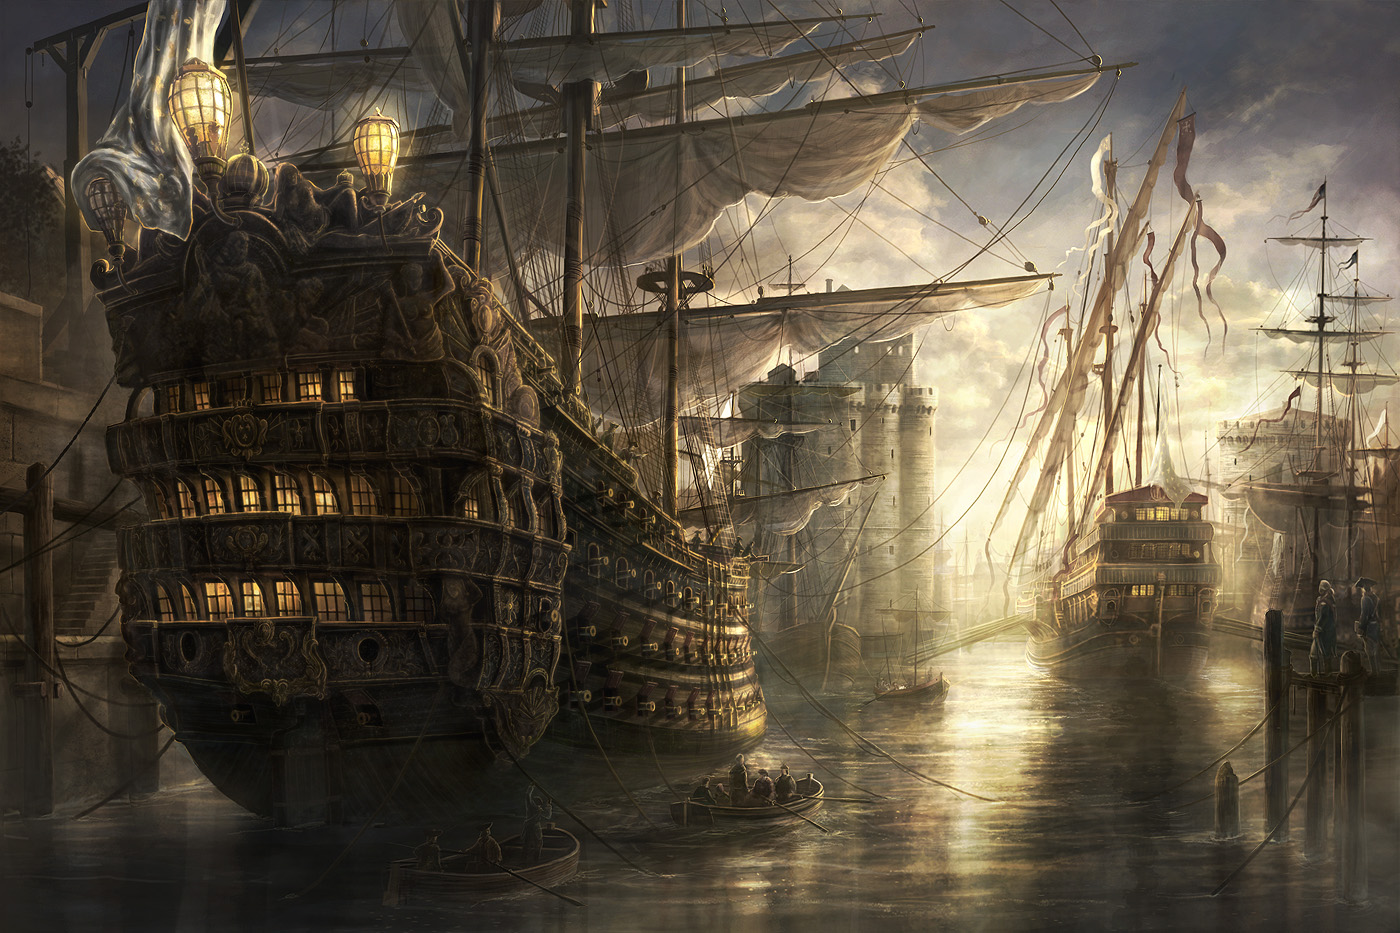
\includegraphics[width=\columnwidth]{La_Rochelle_by_Radojavor}
\end{figure}

\section{Lexicon} 

\section{Adventure Sites}

\end{multicols}





%%%%%%%%%%%%%%%%%%%%%%%%%%%%%%%%%%%%%%%%%%%%%%%%%%%%%%%%%%%%%%%%%%%%%%%%%%%%%%%%%%%%%%%%%%%


%%%%%%%%%%%%%%%%%%%%%%%%%% CHARACTER CREATION %%%%%%%%%%%%%%%%%%%%%%%%%%%%%%%%%%%%%%%%%%%%%%%%%%%%


%%%%%%%%%%%%%%%%%%%%%%%%%%%%%%%%%%%%%%%%%%%%%%%%%%%%%%%%%%%%%%%%%%%%%%%%%%%%%%%%%%%%%%%%%%%



\chapter{Character Creation}\label{chargen}
\pagecolor{gray}\afterpage{\nopagecolor}



\newpage
\pagecolor{gray}\afterpage{\nopagecolor}
\fontfamily{pzc}
\selectfont
%\begin{figure}[h]
%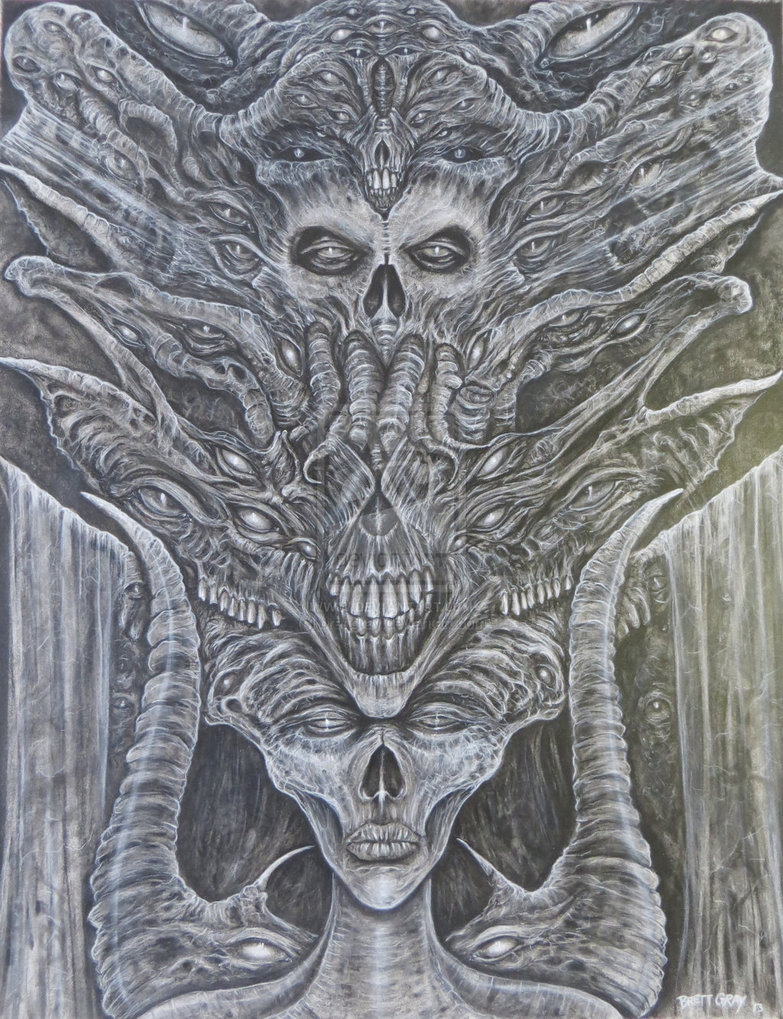
\includegraphics[scale=0.3]{priestess}
%\end{figure}
Birds chirp and the sounds of a flute hum in the atmosphere. The party comprises of Maden Rak, Exeter and Victoria. They travel through the Violet Forest to the Town of Bodmin. 

``Do you hear that?'' 

``I smell Elf.''

On a tree sits an Elf playing a flute. He is fully donned in black and brown leather armour. Over his face is a bandana. His pointed ears stand out prominently. 

``That is...'' before being interrupted by the Elf.

``Maden Rak. Special Forces Commander of the Midgaardian Roaches. Servant of the Dark. Hunter of Elves, murderer of women and children. Twice decorated for valour on the field of battle.'' He claps.

``Caeryn, son of a whore.''

``I've long awaited our meeting. Laid plans, set traps... And now you appear in my forest of your own volition.''

``We are here to bring to justice the Kingslayer and those who aid him. You will rot in a Midgaardian jail!''

``Good luck. This is our land. You will not win here.''

``Since when did the Elves hire professional killers to do their dirty work. The Elves have fallen low.''

``King or beggar, whats the difference? One Human less.''

``Dont make a big deal of the race thing.''

``Yet race is the very reason we fight! We have pointed ears, you have rounded. We have long lives, you have short. Yet you multiply quickly, like vermin, but die just as easily.''

``This is not about race, or freedom, or vengeance. You just refuse to see the obvious truth.''

``And what is that obvious truth?''

``That you are just being used by others.''

``That was a thing of the past! We shall not be used again.''

``Enough of this piss!'' Maden Rak throws a knife at the Elf, who then dodges clumsily in surprise, regains his footage, and then runs up to higher ground using the cover of archers. 
\normalfont

\newpage
\begin{multicols}{2}
This chapter goes through the process of creating a character in the world of Haeckel. There three ways of making characters. 

The basic method that is faster but has reduced options. I chose to build this system so that GMs could use it to help people quickly make characters on the fly such as when GMing in real life with a new gaming group. In this situation you often dont have the time to spend an hour (or more) on character creation.

It makes a party of Humans that are relatively skilled - being of the 1st level.   

And the advanced method which takes abit longer (and involves some reading) but more options. 

Characters built using either system are pretty much the same power level so the only key factor when choosing which to use is how much time you wish to spend making your character. 

The final system is the 0th level system. It makes a party of characters that are trained in a profession but not in adventuring. This system is for relatively mundane characters to be thrown in over their heads in some dire situation, as the GM requires. 

\section{Basic System 1st Level}

\begin{enumerate}
    \item The ability scores are: Strength (STR), Dexterity (DEX), Constitution (CON), Intelligence (INT), Wisdom (WIS), and Charisma (CHA). Record these down using the short hand version in brackets. 
    \item Roll 4d6 drop lowest for each ability score. Check the table below to see the 'ability score modifiers'. This number is based off your Ability Score and is the number that affects your dice rolls. 
    \item In the Basic System you default to a Human. Pick any Ability Score and increase it by +2.  
    \item Choose your class. Your options are: Fighter (STR), Wizard (INT), Rogue (DEX) and Cleric (WIS). Read the page on Core Classes. If you are a beginner player I highly suggest picking the Fighter class; however the Rogue and Cleric are okay for beginners too. I suggest only picking the Wizard class if you are an experienced player or want an additional challenge.
    \item Choose two ability scores to be Primary Attributes (this includes the bonus from being Human, as most other races would only get a choice of 1 Primary Attribute. Your class determines your third Primary Attribute. Your Primary Attributes represents the type of tasks you are best at solving while under pressure or with immense risk, and thus in a significant way shape the kind of character you have.
    \item Pick one equipment starting package. They are described below. Make a note of how much the package weighs. 
    \item You now need to calculate Carrying Capacity. This is equal to your Strength Ability Score. If Strength is your Primary Attribute you gain an additional +4. Likewise, if Constitution is one of your Primary Attributes you gain an additional +4 (stacking with the Strength bonus). For example, a Character with 16 Strength, and has a Primary Attribute of Str AND Con would have a carrying capacity of 24 (16+4+4).
\end{enumerate}

\begin{tabular}{l | r}
    Ability Score & Ability Modifier \\
    \hline
    18 & +3 \\
    16-17 & +2 \\
    13-15 & +1 \\
    9-12 & 0 \\
    6-8 & -1 \\
    3-5 & -2 \\   
\end{tabular}

%\begin{tabular}{l | c | r }
%Fighter Archetypes & Package & Space \\
%\hline
%Swordsman & Blah & 0 \\
%Archer & Blah & 0 \\
%Pikeman & Blah & 0 \\
%Axewielder & Blah & 0 \\
%\end{tabular}
%
%\begin{tabular}{|p{1.5cm}|p{5cm}|p{1cm}|}
%Rogue Archetypes & Package & Space \\
%\hline
%Lovable Rogue & Blah & 0 \\
%Burgler & Blah & 0 \\
%\hline
%Thug & Blah & 0 \\
%\hline
%Explorer & Crossbow, case with 20 bolts, short sword, 2 throwing daggers, sturdy leather armor, tanned brown cloak, thick tunic and pants, leather belt, low boots, backpack, 2 large treasure sacks, 50' rope, tinderbox, lantern, small hammer, 12 iron spikes, 2 flasks of military oil, wineskin, 2 weeks’ iron rations, 3gp & 0 \\
%\hline
%\end{tabular}
%
%\begin{tabular}{l | c | r }
%Cleric Archetypes & Package & Space \\
%\hline
%Priest & Blah & 0 \\
%Crusader & Blah & 0 \\
%Inquisitor & Blah & 0 \\
%Witch Hunter & Blah & 0 \\
%\end{tabular}
%
%\begin{tabular}{l | c | r }
%Wizard Archetypes & Package & Space \\
%\hline
%Witch & Blah & 0 \\
%Scholar & Blah & 0 \\
%Hedge Mage & Blah & 0 \\
%Monk & Blah & 0 \\
%\end{tabular}

\section{Advanced System 1st level}

\begin{enumerate}
    \item The ability scores are: Strength, Dexterity, Constitution, Intelligence, Wisdom, and Charisma. 
    \item Roll 4d6 drop lowest for each ability score.
    \item Choose your race. This may affect your ability scores. 
    \item Choose your homeland, and background.
    \item Choose your class. You can pick from any of the Core Classes or Campaign Classes. Your MAX HP is determined by your class choice and current Constitution ability modifier.
    \item Pick one sphere as your primary sphere.
    \item Pick one feat. The flaws are for more experienced players who would like an additional challenge.
    \item Choose your equipment. For fast play choose a starting package.
    \item Optionally pick a deity to follow. 
    \item Optionally choose a Faction that you aspire to join. 
    \item Optionally choose an Important Character for your character to know about and may want to be involved with. 
\end{enumerate}


\section{0th Level}

\begin{enumerate}
    \item Roll 3d6 for each ability score: Strength, Dexterity, Constitution, Intelligence, Wisdom, and Charisma.
    \item Roll 1d4 for health points, and add your Constitution modifer, as seen in the table above.
    \item Roll on the profession table to randomly determine your profession. This also determines your starting items.
    \item Choose your race. 
    \item Choose 1 ability score to be your Primary Attribute. Or choose 2 ability scores if you are a Human. 
\end{enumerate}

The way this works is basically: if a character survives the first adventure, they become a 1st level character. They may choose a class as per the usual rules. The weapon they used most during the adventure is the weapon they are proficient with at 1st level - unless they're a fighter, in which everything is proficient. 

\end{multicols}



%%%%%%%%%%%%%%%%%%%%%%%%%%%%%%%%%%%%%%%%%%%%%%%%%%%%%%%%%%%%%%%%%%%%%%%%%%%%%%%%%%%%%%%%%%%


%%%%%%%%%%%%%%%%%%%%%%%%%% RACES %%%%%%%%%%%%%%%%%%%%%%%%%%%%%%%%%%%%%%%%%%%%%%%%%%%%


%%%%%%%%%%%%%%%%%%%%%%%%%%%%%%%%%%%%%%%%%%%%%%%%%%%%%%%%%%%%%%%%%%%%%%%%%%%%%%%%%%%%%%%%%%%

\chapter{Races}\label{races}
\newpage
While Humanity dominate the continent the demi-human races still flourish in varying forms. There are no more true demi-human civilisations anymore and all that exist are either embedded within existing pan-Human societies or are isolated and small in size. 

\section{Approaches}
\subsection{Everyone is Human} This approach has a number of strengths. The first is that you reduce the complexity of the characters so that you can focus on other aspects of the game. For instance, you do not need to deal with the senses of the various races. Another advantage is that since everyone is Human, darkness becomes a more effective tool at creating atmosphere simply because forms of dark vision are not available. This approach is also effective because it allows you to introduce other races slowly - thus their distinction from Humans is more apparent and from a new player experience sense possibly more powerful. The players first experience with a demi-human race will pretty much set the tone and impression that the player has for that race from then on. 

%We're not treating demi humans as basically humans but with a pallet swap. They will significantly influence the character's experience - for example Gnomes have a tight knit community and will have roleplay ramifications.
%
%Races have various racial vulnerabilities and resistences. This has the effect of promoting a counter system in the game.
%
%We're drawing from some of the ideas from old school gaming. Drow have infravision (heat vision), Halflings have deadly accuracy, Elves see vast distances (10x greater than Humans), Dwarves are highly resistent to magic and are the only ones who can use Magical Returning Warhammers.
%
%Races have an affect on resource management. Halflings eat alot. Wood Elves cant eat meat. Gnolls must only eat meat (and are cannibalistic). Dwarves must have a supply of alcohol.

\section{Overview}

\begin{tabular} { l p{4cm} l l l }
    Race & Ability Scores & Weaknesses & Strengths & Senses \\
    \hline
    Dark Elf & \\
    Dwarf & +2 CON, -2 CHA & None & Resist (Poison, Magic) & Deepvision 120ft\\
    Duergar & +2 CON, -4 CHA & Holy & Resist (Poison, Paralysis) & Deepvision 120ft\\
    Fire Giant & +4 STR, -2 INT, -2 CHA & Cold & Resist (Fire), Large & \\
    Gnoll & +2 CON & Resist (Disease) & Fear (Fire) & Scent 30ft\\
    Gnome & +4 INT, -2 STR & None & Resist (Illusions) & Enhanced Hearing\\
    Half Elf & Any +2 & Iron & None & Low Light Vision 30ft\\
    Halfling & +2 CHA, -2 STR & Small & None & Enhanced Taste\\
    Human & Any +2 & None & None & \\
    Minotaur & +2 STR, +2 WIS, -2 DEX, -2 CHA & None & None &  \\
    Tzuchi & +2 INT, +2 CON, -2 STR & Holy & Resist (Poison) & Smell Blood 30ft\\
    Wood Elf & +2 DEX, +2 WIS & Iron & None & Twilight Vision, Farsight\\
\end{tabular}

\newpage
\begin{multicols}{2}

\section{Dark Elf} Two warring tribes have chosen Haeckel's killing fields as their arena. Each is the other's prey, each the other's predator. On Haeckel many warriors awake to find themselves in a new and more deadly environment, stalked by a strange enemy. All alone in a strange world, he must do what he knows best survive against all odds. These are the tales of terror that the Dark Elves bring. The Dark Elves are killing machines that hunt and kill their prey, either from afar using their infravision, or in hand to hand combat with vicious weaponry. They have a warriors code that detail the protocols of the Hunt, and access to superior class of weaponry not available to most others - such as Repeater Crossbows. The Dark Elves worship the Death God - for when they die, they believe they must answer to Him.

\paragraph{Homelands}

\begin{framed}\centering
In general, Dark Elves are best suited for players who wish to do solo adventures. That is why we intend for them to be more powerful than the other player races, and be a combination of the Fighter and Ranger class. It is intended that Dark Elves have no way to deal with traps inherently - that is their weakness to offset their combat abilities. If one was to use Dark Elves in normal parties, I would suggest limiting their access to only those characters whom roll high ability scores (to reflect their rarity and prize of those players lucky enough to roll up one). In this way they are balanced through rarity.
 \end{framed}


\section{Dwarf}

One of the so called ancient races, their greed and grudges are legendary.     

    \paragraph{Ability Scores} +2 CON, -2 CHA.
    \paragraph{Senses} Deepvision 120ft, Smell Gold 30ft. 
    \paragraph{Resistances} Poison \& Magic.  
    \paragraph{Weaknesses} 
    
\section{Duergar}
    Duergars tend to lead lives of never ending turmoil and often seen to be existing for the purpose of the manufacture of wealth through unending labour. Duergars are known for their cruelty, strength and wealth. Their caravans have been seen in every corner of Haeckel for they are not picky with who they ply their trade. No obstacle daunts a gray dwarf who has settled on a goal. Duergar may not display much loyalty to anyone other than themselves, but they never leave a job half done. Their avaricious, short-tempered, sullen, violent, and ungrateful nature is only matched by the redeeming virtues of courage and determination. An interesting aspect to the Duergar is their almost universal hatred of thieves. Many of spent the better part of decades mastering the art of identifying them and hunting them down. Some of the greatest innovations in locks and traps has been made by the Duergar. 
    
    \paragraph{Ability Scores} +2 CON, -4 CHA.
    \paragraph{Senses} Deepvision 120ft, Sense Hidden Foes 10ft
    \paragraph{Resistances} Poison \& Paralysis
    \paragraph{Weaknesses} Holy Weapons. 
    \paragraph{Alignment} Always Evil. 
    

\end{multicols}    

\newpage
\changepage{9cm}{9.4cm}{-4.7cm}{-4.7cm}{}{-4.5cm}{}{}{}
%\noindent\rule{\textwidth}{\textheight}
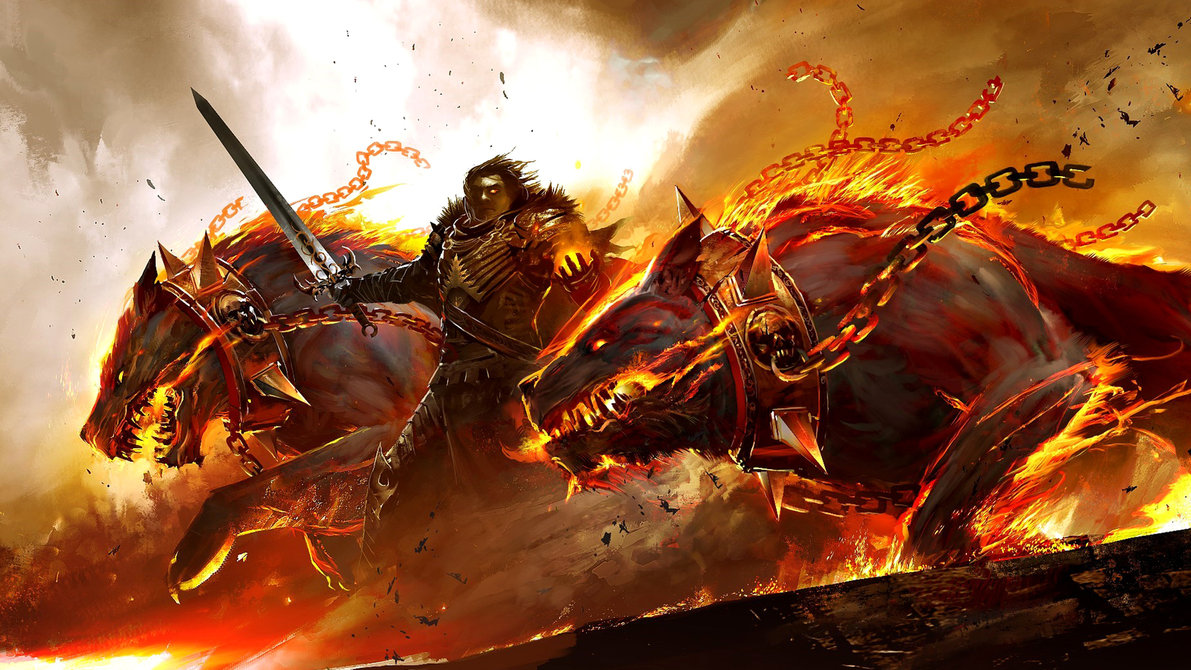
\includegraphics[width=\textwidth,height=\textheight]{firegiants}
\newpage

%restoring the standard settings
\changepage{-9cm}{-9.4cm}{4.7cm}{4.7cm}{}{4.5cm}{}{}{}

\begin{multicols}{2}
\section{Fire Giant}
    \paragraph{Ability Scores} +4 STR, -2 INT, -2 CHA.
    \paragraph{Senses} Fire and smoke does not obscure vision.
    \paragraph{Resistances} Fire.
    \paragraph{Weaknesses} Cold. 
    \paragraph{Alignment} Always Evil. 
\section{Gnoll} Creatures of Chaos, the terrible and barbaric Gnolls are intelligent beasts for whom the laws of nature are the moral precepts by which they abide. Forget the blessings of charity. Forget the divinity of faith. The Gnoll is a product of the raw undiluted power of nature. There is no Gnoll civilisation, past or present. The Gnoll is profoundly capable of adapting to its natural environment in Haeckel because of their impressive ability to resist disease. Despite their distasteful ethics by Human standards, Gnolls have adapted to the socio-cultural environment of Urban life. Their talents lend them uniquely to being exceedingly good bounty hunters, mercenaries and brutal assassins. 

    \paragraph{Ability Scores} +2 CON
    \paragraph{Senses} Scent 30ft.
    \paragraph{Resistances} Disease.
    \paragraph{Weaknesses} Fear (fire)

\paragraph{Pack} They may not have henchmen. In exchange, the Gnoll is part of a Pack that act as a territorial unit governing some large region. The larger the region, the larger the pack. The influence of the Pack protects the Gnoll from the Mob. The Humans leave the Gnoll alone, and the Gnoll does the same for the good of the pack. 

\paragraph{Baying for Blood} A gnoll's howl can be heard from several miles away. They use it as a way to communicate with each other. Often they use it for a rallying cry to gather the pack to hunt and to mark territory (warn others off). 

\paragraph{Moon Sensitivity} 

\section{Gnome} Often said to be the most intelligent race on Haeckel, they are few in number and often in positions of influence or wealth. Gnomish scholars are highly valued by the Human noble classes as advisors due to their "hyper-intellect". It is commonly thought that there is no equal in this field. The reality is that both Tzuchi and Wood Elves come a close second in intellect and if it were not for various reasons those races would pose a significant threat to the gnomish domination in the scholarly persuits. 

Gnomes are very famous for their black humour. They are great connoisseurs of gems and are the best gem carvers in the known world. They also dominate the field in expertly crafted leather goods. Gnomish boots are a quality product that every race enjoys (except the giant races). There is also a warrior class of Gnomes whom are seen to be expert crossbowmen. In many regions they hold sharpshooter tournaments. 

    \paragraph{Ability Scores} +4 INT, -2 STR.
    \paragraph{Senses} Enhanced Hearing. 
    \paragraph{Resistances} Illusions.
    \paragraph{Weaknesses} 
    
    \paragraph{Hyper-Intellect} Gnomes get a 25\% discount on the experience required to level up. 

\section{Half Elves} 

% They are a tasty stew of triumph and tragedy. 

    \paragraph{Ability Scores} Any +2. 
    \paragraph{Senses} Low Light Vision 30ft.
    \paragraph{Resistances} 
    \paragraph{Weaknesses} Iron.
    
\section{Halfling} Halflings within Haeckel are usually refuges who have fled from ghul. Within Haeckel they usually find themselves working as housekeepers, kitchen aids, gardeners. They drink like dwarves but lack the same tolerance as them. They love music, only the music they love is hated by all other races. Their ethnic food is loved, they seemed to have mastered the culinary secrets of corn and cheese. They are often scapegoated and bullied, which results in gangs forming to protect halfling communities. Due to their extensive gardening techniques, the gangs they formed became drug pushers. They talk of an ancient halfling kingdom (resembling mayan/aztec) only that kingdom was taken over by larger barbarian tribes and many of the halflings became the sacrifices. Halflings can be easy going, friendly, very trusting of others. Drugs and alcohol brings out the darker side of their personalities; they become belligerent, vengeful and abusive.

    \paragraph{Ability Scores} +2 CHA, -2 STR.
    \paragraph{Senses} Enhanced Taste.
    \paragraph{Resistances} None. 
    \paragraph{Weaknesses} None.
    \paragraph{Voracious Eaters} Halflings are probably the most restricted race in terms of their diet. Eating bad food causes Halflings to have a significant morale penalty. 
    \paragraph{Sling Sharpshooters} This is such a pervasive sport in Halfling culture that virtually all are pretty good at it before reaching adolescence. 

\section{Human} Humans are the standard by which all other races must be measured. They form the almost absolute majority of Haeckel's population, nonhuman races are commonly known only through rumour or legend. Human's fill every niche in society and represent a wide spectrum of cultures and ethnic groups. Traits within those ethnic groups and or cultures will reflect statistically. Homelands: Human communities can be found in every settled domain. That is, as far as settled domains go. Some domains have no permanent human settlements, though human encampments or nomadic elements may exist.

\begin{figure}[h]
\includegraphics[width=\columnwidth]{lumberjack10}
\end{figure} 

    \paragraph{Ability Scores} Any +2.
    \paragraph{Senses} Nothing special.
    \paragraph{Resistances} Nothing. 
    \paragraph{Weaknesses} Nothing.
    
    \paragraph{Ingenuity} Most characters get a choice of one Primary Attribute in addition to the one granted from their class choice. Instead, the Human character gets to pick two (for a total of three). 
    
    \paragraph{Regional Background} More so than any other Race, Humans are defined more by their homeland and social class than as a Human. 



\section{Minotaur}

Minotaurs are terrible beastmen whose vicious charges on the battlefield have been known to haunt the nightmares of many a fallen and crippled Knight. Despite being monsters, they are a conflicted race. Minotaurs cannot reproduce with their own race for every Minotaur is male, thus they can only spread the seed of their race by polluting the wombs of Human women. In ages past this was primarily done in violent rites of blood sacrifice but this culture has almost died out. This all in all has led to their rarity in Haeckel. Adding to these problems their bovine mouths make it very difficult for them to communicate with the other races. But most tragic fact though is that despite their appearance, on the inside Minotaur's heart and soul shines with an inner light.

The two largest societies of Minotaurs exist in Abyssimiar and Ubris Furor, though there are known to be Minotaurs affected by the Phex that still live in the Old Kingdom of Avalonia. 
 
\begin{figure}[h]
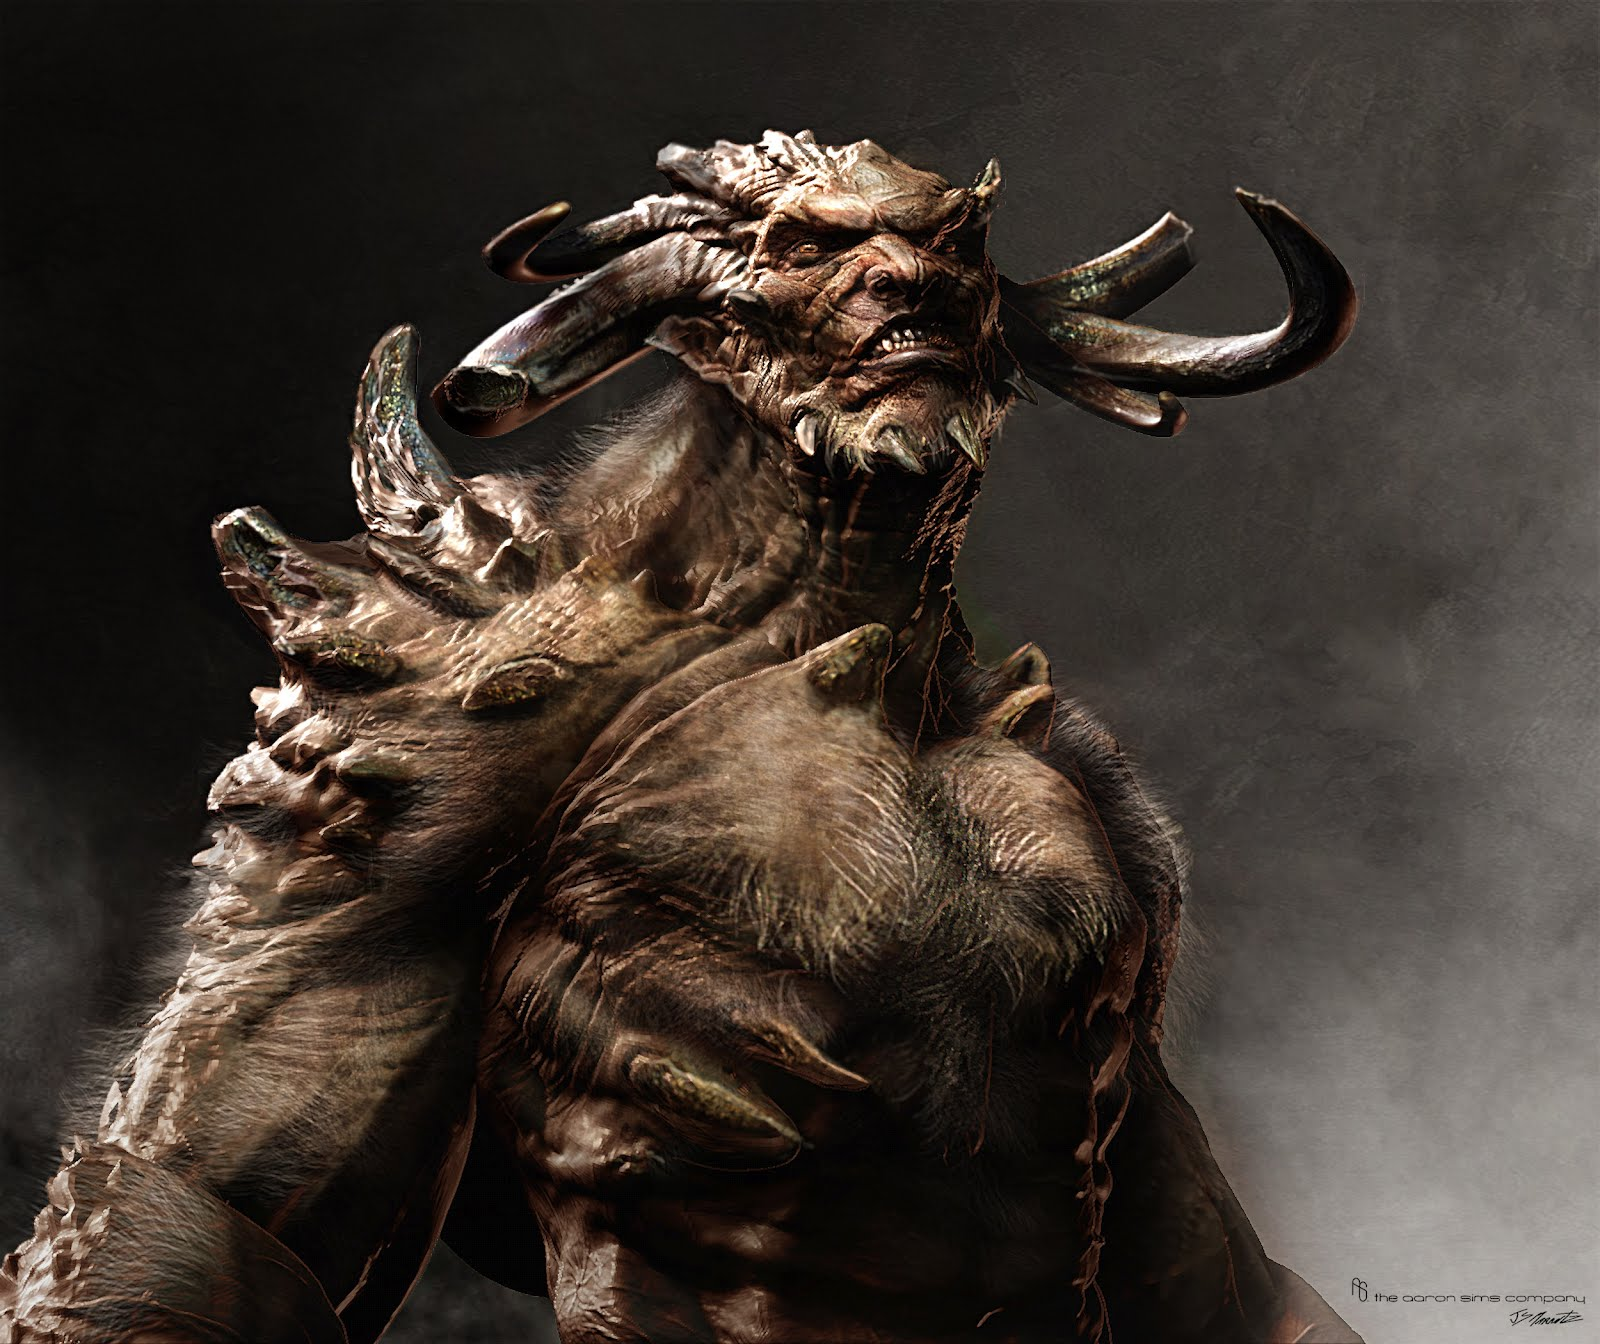
\includegraphics[width=\columnwidth]{Minotaur_sketch}
\end{figure}    
    \paragraph{Ability Scores} +2 STR, +2 WIS, -2 DEX, -2 CHA.
    \paragraph{Senses} 
    \paragraph{Resistances} 
    \paragraph{Weaknesses} 
    
    \paragraph{Alignment} Always Good. 
    \paragraph{Temper} 

\section{Tzuchi}
    A mysterious and foreign race of Snakemen native to the Southern Continent. They are exceedingly rare to see in the fallen Imperial provinces of Haeckel. The Tzuchi are cold blooded sociopaths that are unable to emphathise with warm blooded creatures. In their own homeland they are at the core of the Theocratic religious caste there. Tzuchi whom are on Haeckel are usually on trade expeditions or as part of political envoys. Behind the scenes however Tzuchi aim to covertly infiltrate and dominate the criminal underworld of Haeckel. 
    
    \begin{figure}[h]
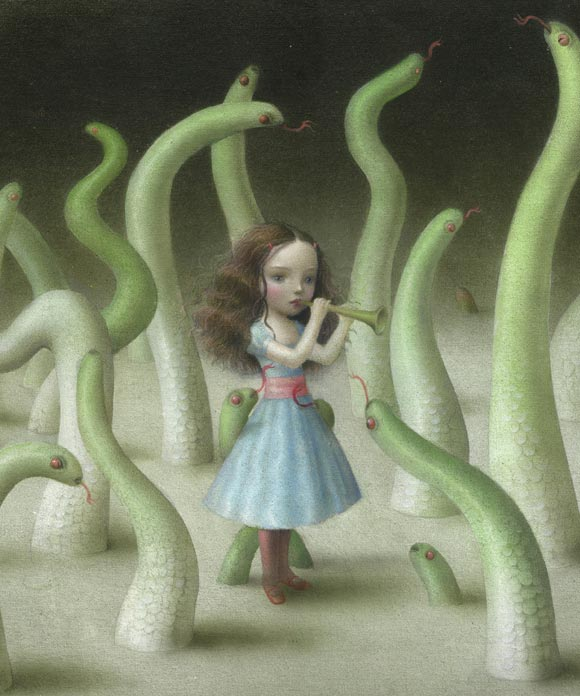
\includegraphics[width=\columnwidth]{incubi-celesti}
\end{figure}
    \paragraph{Ability Scores} +2 INT, +2 CON, -2 STR
    \paragraph{Senses} Smell Blood 30ft, Smell Fear 30ft.  
    \paragraph{Resistances} Poison.
    \paragraph{Weaknesses} Holy Weapons. 
    
    \paragraph{Alignment} Always Evil. 
    
    \paragraph{Venomous Bite} The bite of a Tzuchi causes delirious hallucinations in the affected victim. It is said that they see mad visions of a Snake God that torments their nightmares for weeks on end. 
    \paragraph{Sociopathy} Tzuchi are virtually incapable of discerning the emotions or empathising with warm blooded creatures. Any attempt to sense this will fail or worse end with horrific failure.
    \paragraph{Order of the Faith} Tzuchi's theocratic life imposes severe limitations on the behaviour of a Tzuchi. 
    
    The Tzuchi Tribune aim to significantly improve Human-Tzuchi relations and thus enforce that Tzuchi be honest in all their dealings and do what it takes to promote this cause. 
    
    A Tzuchi who is caught being dishonest is most likely going to be eaten by his fellows; thus in any deception it is highly suggested that Tzuchi displace responsibility of conspiracies to others, and to make sure there is always a fall guy as well as any necessary cover stories.
    
    A Tzuchi who fails in these duties is seen as incompetent and thus unworthy to live. Social Darwinism is the status quo in the vicious and cutt-throat competitive Tzuchi Society.  
    \paragraph{Hidden Agenda} Whether for real or imagined reasons, nobody trusts a Tzuchi. 
    
\section{Wood Elf} Wood Elves have had perhaps the most tragic and turbulent histories in Haeckel. At their height they dominated the continent and were seen almost as a master race. The legends speak of the Wood Elves having direction connections with the deities before the Dread Gates existed. 1300 Years ago Humans migrated onto the continent from a faraway land and displaced the status quo. At their lowest the Wood Elves were sold as prized slaves. Their holding onto paganic Old Ways has led them to be scapegoated in certain regions. In others they are held with high regard. 

In regions where there is deep seated discrimination and racism towards the Wood Elves they have organised into guerillas and waged 100 year wars against the Tyrants. Rob merchant caravans, plunder and burn villages, and kill. Instead of finding a peaceful solution, many humans send troops to fight them. In most cases the Tyrant will realise the economic cost imposed upon them for carrying out their hatred and call for peace. Armed rebellion, resistance, and assassination of Human leaders is considered a morally acceptable position of Elves in troubles. Wood Elves find the Human notion of the Divine Right of Kings amusing – whereas this idea is deeply ingrained in most Human cultures. 

Their mobility, sword styles, and ability to disengage combat much more safely than other races makes them some of the best skirmishers in the world. From the tactical situations, to social situations to character development, Wood Elves will have a unique look and feel in real gameplay terms.

\paragraph{Ability Scores} +2 DEX, +2 WIS.
\paragraph{Senses} Twilight Vision, Farsight
\paragraph{Resistances} 
\paragraph{Weaknesses} Iron. 

\paragraph{No Teamwork} Elves do not gain bonuses from flanking, nor can they be flanked.

\paragraph{Martial Arts} Elves do not fight in regimented formations. They require much more space due to the elegant moves of their various fighting styles. Thus for the purposes of combat they count as requiring 10ft by 10ft.  

\begin{framed}\centering
It is intended that Elves whom live long enough eventually become master duelists who are unrivaled in martial prowess. While their Martial Arts trait may not seem like much, this is actually a pretty significant disadvantage in the gameplay of Haeckel RPG. This disadvantage is balanced out by the fact they have no penalty to ability scores and will have the opportunity to gain some of the best combat feats available to any race.   
\end{framed}

\end{multicols}






%%%%%%%%%%%%%%%%%%%%%%%%%%%%%%%%%%%%%%%%%%%%%%%%%%%%%%%%%%%%%%%%%%%%%%%%%%%%%%%%%%%%%%%%%%%


%%%%%%%%%%%%%%%%%%%%%%%%%% CORE CLASSES %%%%%%%%%%%%%%%%%%%%%%%%%%%%%%%%%%%%%%%%%%%%%%%%%%%%


%%%%%%%%%%%%%%%%%%%%%%%%%%%%%%%%%%%%%%%%%%%%%%%%%%%%%%%%%%%%%%%%%%%%%%%%%%%%%%%%%%%%%%%%%%%



\chapter{Core Classes}\label{coreclasses}
\pagecolor{gray}\afterpage{\nopagecolor}
\newpage
\pagecolor{gray}\afterpage{\nopagecolor}
\fontfamily{pzc}
\selectfont
Co-Consul of Ablon enters the Office and the General Autorius sits at his table, golden goblets of wine and a plate full of grapes rests easy in front of him. 

``We had an agreement, that we'd share all revenue.''

``Yes''

``Hereopolis has agreed to give you 20,000 pounds of gold. I want my share.''

``Who told you this?''

``You deny?''

``Who told him.''

``I have spies among his people.''

``If Herod is kind enough to give me a gift, what business is it of yours? A gift is not revenue.''

It is not a gift, it is a bribe. For political and military favours. The cost of which favours shall be born by the state.''

``Peasantry.''

``Let us be realistic. This arrangement of ours can not work if you seek every opportunity to aggrandize yourself at my expense.''

``Laughter. Aggrandize myself. This from the boy whose so called father has been declared a God.''

``An honour he well deserves.''

``You only did it so you might be known as the Son of a God. You have no accomplishments of your own, so you seek to borrow the glory of others.''

``Its true, it was no accomplishment to defeat you at Mutina.''

``You defeated me? You cowardly little shit. You never left your tent. You have never defeated me, in anything.''

``Gentlemen, lets not get overheated. Im sure we can come to some reasonable agreement. I had hoped that you had learnt some humility and discipline. You are still the same old crude, arrogant, lech that you always were.''

``Thats right. Just the same. The same that is still fucking your mother!''
\normalfont
\newpage

%changing the page design temporarily
\changepage{9cm}{9.4cm}{-4.7cm}{-4.7cm}{}{-4.5cm}{}{}{}
%\noindent\rule{\textwidth}{\textheight}
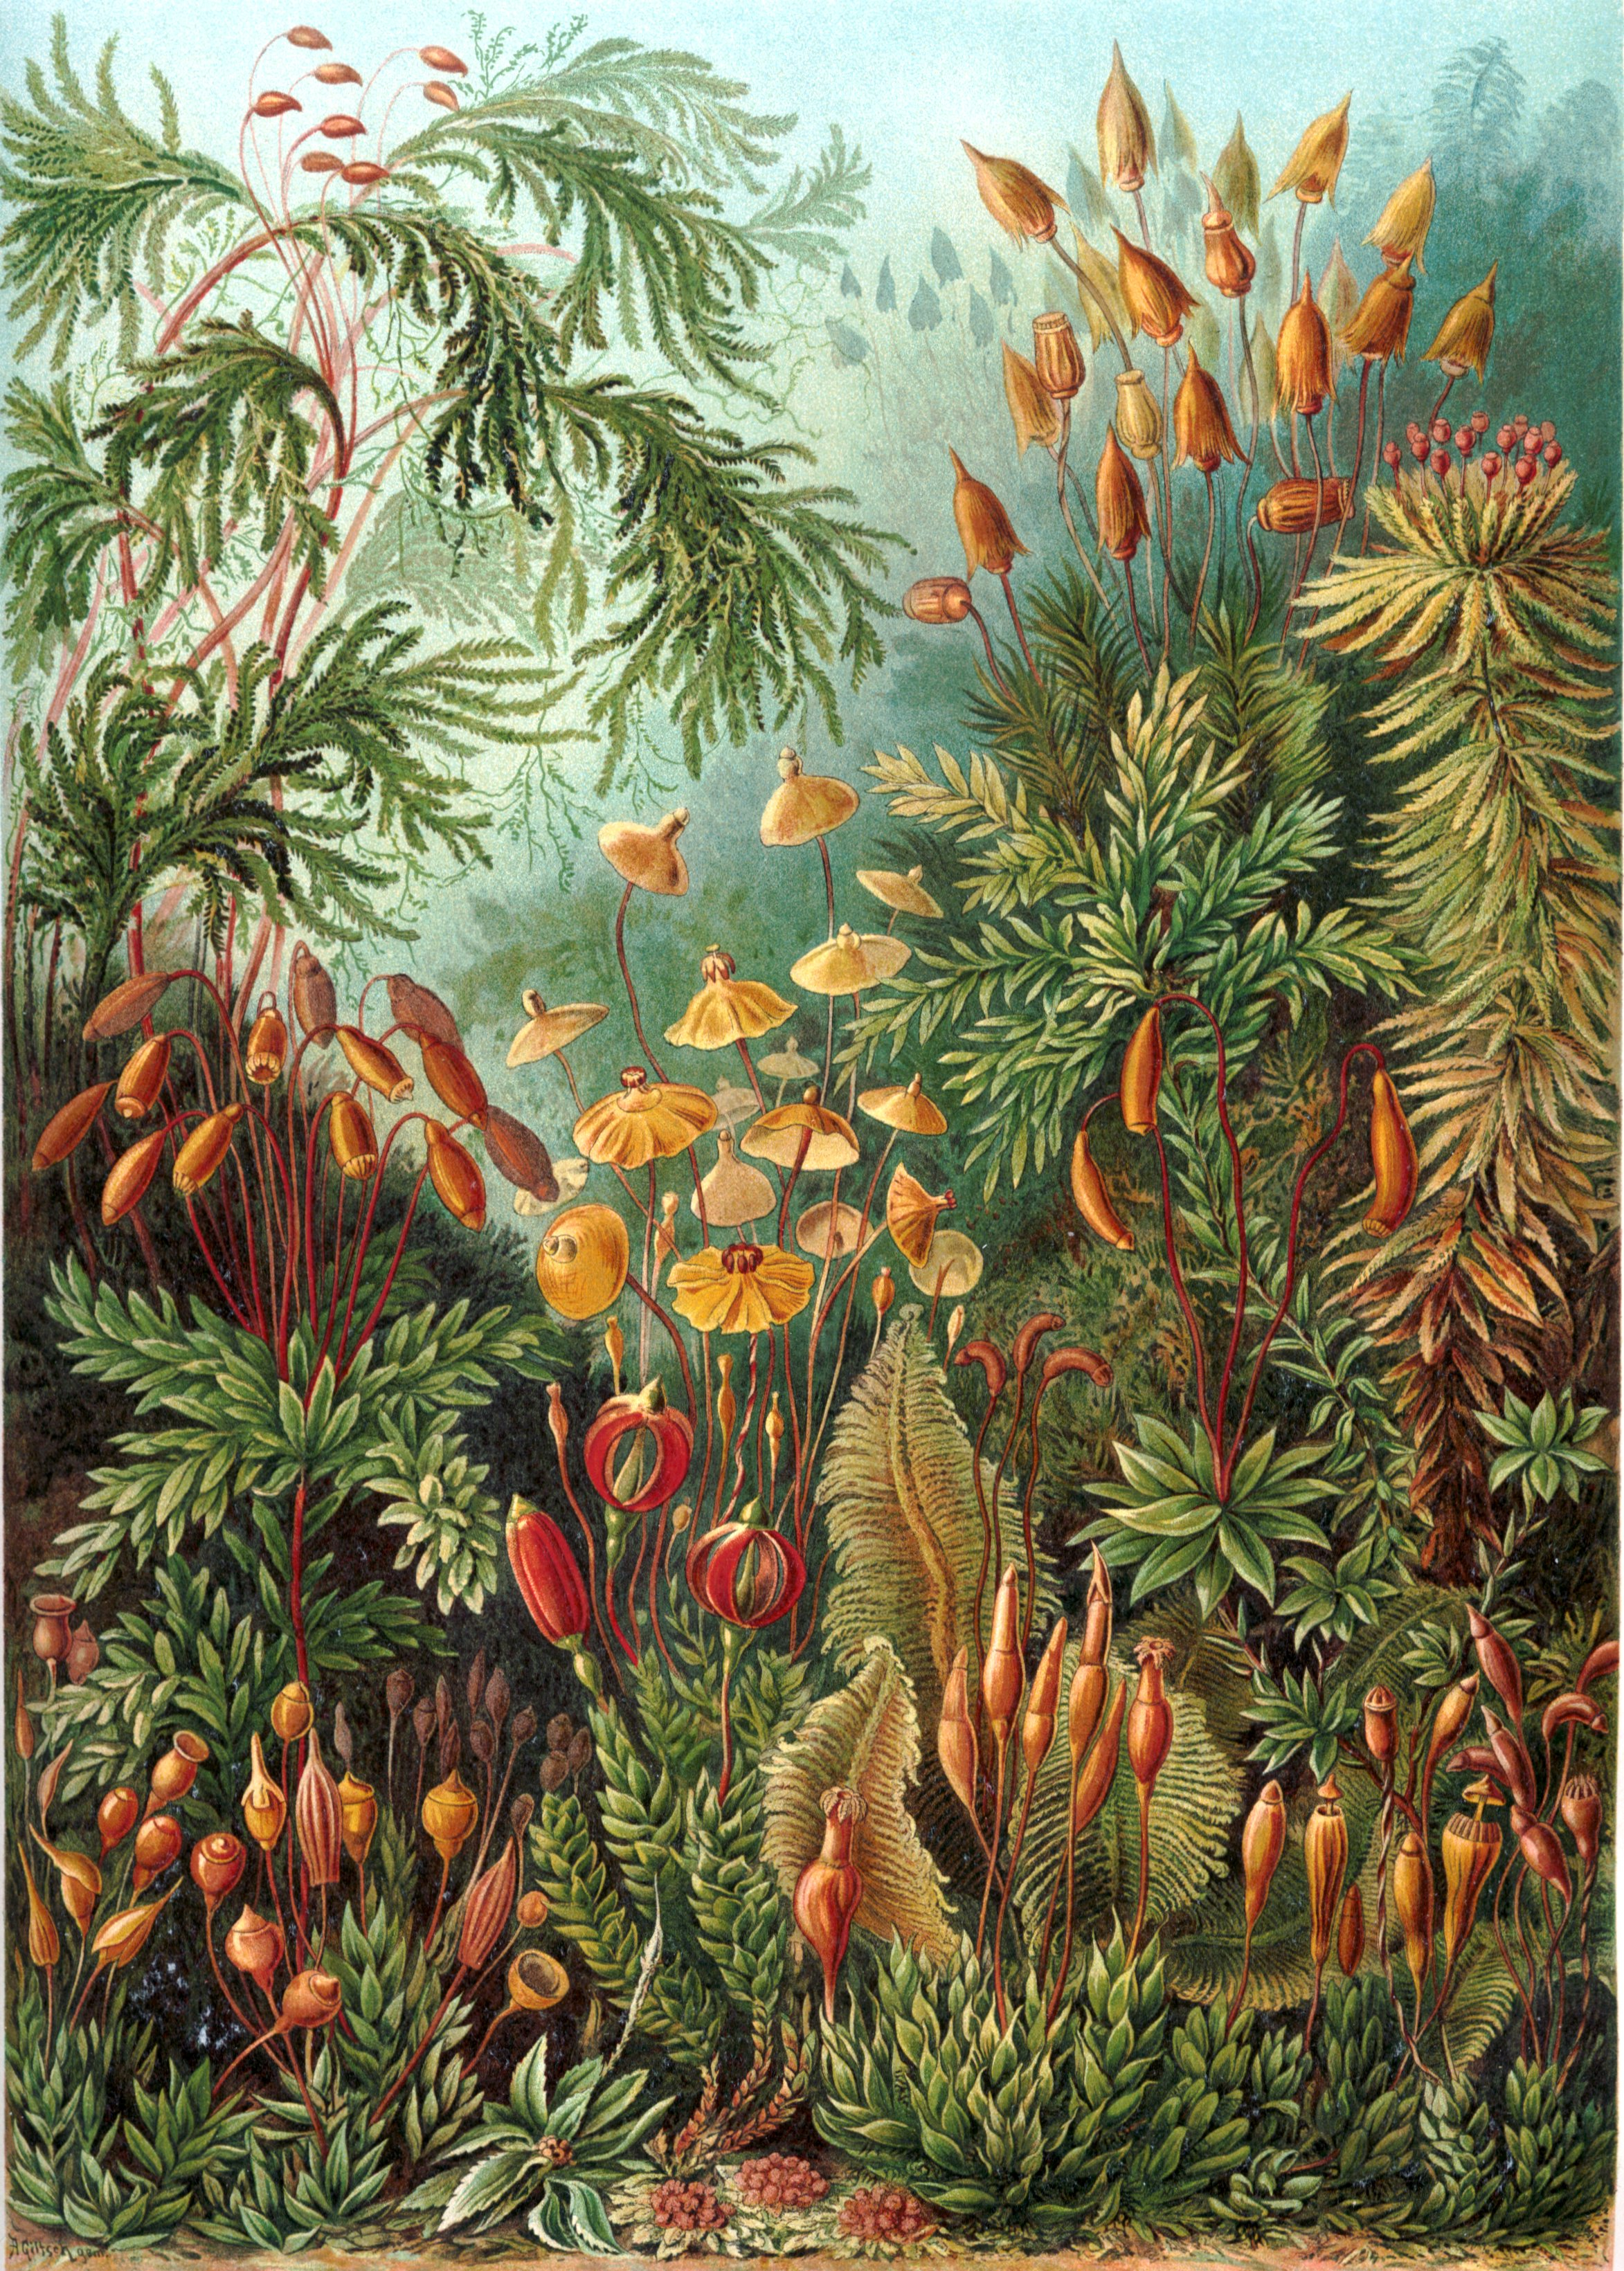
\includegraphics[width=\textwidth,height=\textheight]{Haeckel_Muscinae}
\newpage

%restoring the standard settings
\changepage{-9cm}{-9.4cm}{4.7cm}{4.7cm}{}{4.5cm}{}{}{}

\begin{multicols}{2}
The Core Classes are archetypical classes to the worlds most popular RPG system. They encapsulate problem solving philosophies and a way of playing the game. 

This class system is designed to be extremely simple. It is fundamentally an "open formed gaming" system. I.e. pretty much every character can sneak around, or swim, or climb walls. The difference is that certain characters have additional capabilities above the norm. 

It is very fine to have an entire party composed of Fighters. Having a cleric on the team greatly increases survivability however. 

\section{Fighter} This class is best at solving problems via brute force. They are not just a duelist but are skilled in any form of warfare. 

The Fighter may use any weapon or armour. Their starting HP is 10. Each time they level up they must roll 1d10 to determine the HP gained for that level up. This makes them a very tough class to kill relative to the other classes.

The Fighter class is illiterate but can speak in Common.  

\section{Wizard} They are the late game class. Their starting HP is 4, and they gain 1d4 hp per level up. Most wizards are proficient with no weapons and armour, unless some other mechanic such as Race dictates otherwise. To survive you will have to master using terrain and keeping aware of your surroundings. 

The capabilities of the Wizard are virtually unknown. They are an esoteric class whom start off as a Scholar without spellcasting capabilities and must learn dark secrets to unlock their potential. They are thus not suitable for brief adventures and best suited for campaign play.

As a Wizard you begin knowledgeable in one of the fields of Academia. You have two basic ways to use this. You can ask the GM for advice or information pertaining to the topic, and/or you can use your own knowledge of the topic (relevant to the time period of the game) to your own advantage. 

The Wizard class begins literate in Common and High Common - the language of the nobility classes.  
 
\section{Rogue} Rogues may only wear leather armour and are severely limited in their weapon selection. The most common rogue weapons are Daggers and Shortbows. Their starting HP is 4 and they roll 1d4 each time they level up for extra HP. The rogue class has access to a number of special skills that provides them additional utility. 

Their two principal combat abilities are Backstab and Set Traps. Their utility abilities are: Hide in Shadows, Climb Steep Slopes, and Listen at Doors.

The Rogue class is illiterate but can speak in both Common and Low Common - the language of the criminal underworld. 

\section{Cleric}

Clerics may wear armour and use any weapon. Their starting HP is 8 and they roll 1d8 each time they level up for extra HP. 

The principal advantage of playing a Cleric is that of your involvement with society at large. If you have a local congregation, it is likely that they will come to your aid, and it is expected that you come to theirs in times of need. 

Some Churches become extremely powerful allies. Also, ostensibly, merchants are less willing to rip off Clerics than other classes. This is not a fool proof way of being safe from scams however.  

The Cleric class can read and write in Common and Gothic - an ancient language of religious scripture.

\end{multicols}




%%%%%%%%%%%%%%%%%%%%%%%%%%%%%%%%%%%%%%%%%%%%%%%%%%%%%%%%%%%%%%%%%%%%%%%%%%%%%%%%%%%%%%%%%%%


%%%%%%%%%%%%%%%%%%%%%%%%%% PERSONALITY %%%%%%%%%%%%%%%%%%%%%%%%%%%%%%%%%%%%%%%%%%%%%%%%%%%%


%%%%%%%%%%%%%%%%%%%%%%%%%%%%%%%%%%%%%%%%%%%%%%%%%%%%%%%%%%%%%%%%%%%%%%%%%%%%%%%%%%%%%%%%%%%

\newpage
\chapter{Personality}\label{personality}
\pagecolor{gray}\afterpage{\nopagecolor}
\newpage
\pagecolor{gray}\afterpage{\nopagecolor}
blah blah
\newpage

\changepage{9cm}{9.4cm}{-4.7cm}{-4.7cm}{}{-4.5cm}{}{}{}
%\noindent\rule{\textwidth}{\textheight}
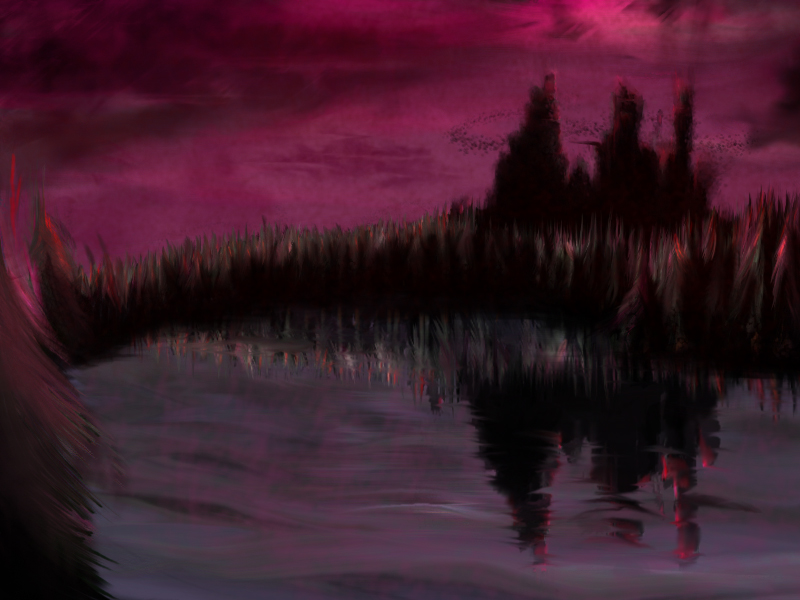
\includegraphics[width=\textwidth,height=\textheight]{Avalonia4}
\newpage

%restoring the standard settings
\changepage{-9cm}{-9.4cm}{4.7cm}{4.7cm}{}{4.5cm}{}{}{}

\begin{multicols}{2}


\subsection{Ethos}
\paragraph{Good}
\paragraph{Evil}
\subsection{Spheres}
Think of your sphere as your birth sign, with power over your deepest thoughts. The reality is that spheres are aspects made manifest by the influences of the esoteric Dread Gates. It is suggested to use Spheres as a way to theme your character and influence his narrative. 

Dont think of spheres as a way to straightjacket your character. They provide no obvious mechanical benefit. It is upto the player to decide how the sphere influences and shapes them. It is possible that multiple spheres are relevant to your character. You have a choice of one sphere and this acts as the primary sphere. The rest would be secondary. 

\begin{tabular}{l|c|r}
    Emotions & Elements & Spiritual \\
    \hline
    Love & Fire & Blasphemy\\
    Hate & Water & Apostacy\\
    Fear & Earth & Despair\\
    Pride & Air & Hatred\\
    Greed & Lightning & Indifference\\
    Lust & Wood & Envy\\
    Apathy & Metal & Sloth\\
    Revenge & Light & Wrath\\
    Honour & Darkness & Gluttony\\
    Glory & Storms & \\
\end{tabular}

\subsection{World View}
\subsubsection{Philosophies}
    \paragraph{Stoicism} "The greatest good was contentment and serenity."
    \paragraph{Hedonism} "Eat, drink and be merry, for tomorrow we die."
    \paragraph{State consequentialism} The moral worth of an action based on how much it contributes to the basic goods of a state.
\paragraph{Ideologies}
\subsection{Politics}
\paragraph{Imperial vs Provincial}
\paragraph{Monarchy vs Republic}
\paragraph{Secular vs Theocratic}
\paragraph{Class conflict}

\end{multicols}




%\chapter{Regional Backgrounds}\label{regionalbackgrounds}
%    \section{Ablon}
%        \subsection{Fashion}
%        \subsection{Stereotypes}
%    \section{Abyssimiar}
%            \subsection{Fashion}
%            \subsection{Stereotypes}
%    \section{Avalonia}
%            \subsection{Fashion}
%            \subsection{Stereotypes}
%    \section{Brouliard}
%            \subsection{Fashion}
%            \subsection{Stereotypes}
%    \section{Nes}
%            \subsection{Fashion}
%            \subsection{Stereotypes}
%    \section{North Wall}
%            \subsection{Fashion}
%            \subsection{Stereotypes}
%    \section{Midgaard}
%            \subsection{Fashion}
%            \subsection{Stereotypes}
%    \section{Ubris Furor}
%            \subsection{Fashion}
%            \subsection{Stereotypes}
            

\chapter{Campaign Classes}\label{campaignclasses}


\pagecolor{gray}\afterpage{\nopagecolor}
\newpage
blah blah blah
\pagecolor{gray}\afterpage{\nopagecolor}
\fontfamily{pzc}
\selectfont

\newpage
\normalfont
%changing the page design temporarily
\changepage{9cm}{9.4cm}{-4.7cm}{-4.7cm}{}{-4.5cm}{}{}{}
%\noindent\rule{\textwidth}{\textheight}
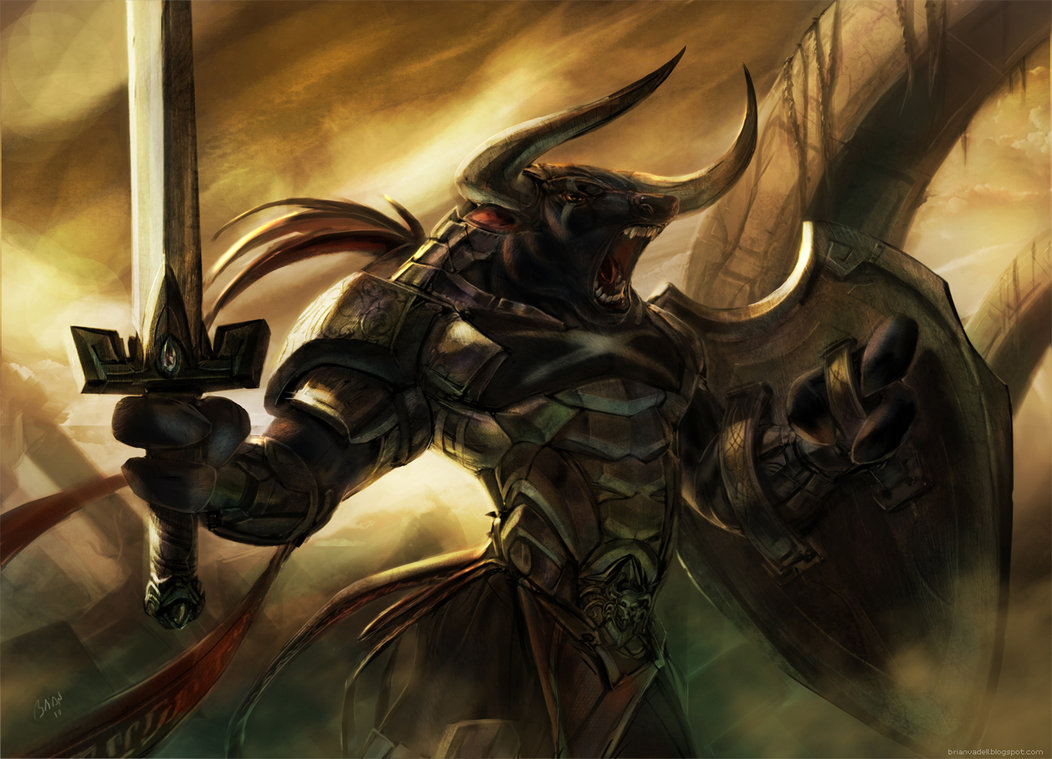
\includegraphics[width=\textwidth,height=\textheight]{minotaur_by_brianvadell}
\newpage

%restoring the standard settings
\changepage{-9cm}{-9.4cm}{4.7cm}{4.7cm}{}{4.5cm}{}{}{}
	These are special classes that build upon the existing core classes in the game. They reflect the influence that the setting has upon the character's own skills and talents. 
	There are essentially two types of Campaign Classes. Those that are tied to some regional background, and those tied to some faction. 
	Each faction provides some campaign classes, which maybe unlocked once they have joined and proved themselves within said faction. 
	Some campaign classes are also limited by what races may enter into it. 
\section{Dying Rat Minotaur} This faction campaign class is dedicated to maximising the lethality of his horns goring into someone on the charge. 

\section{Crusader Minotaur} 

% minotaur_by_brianvadell
%\begin{figure}[h]
%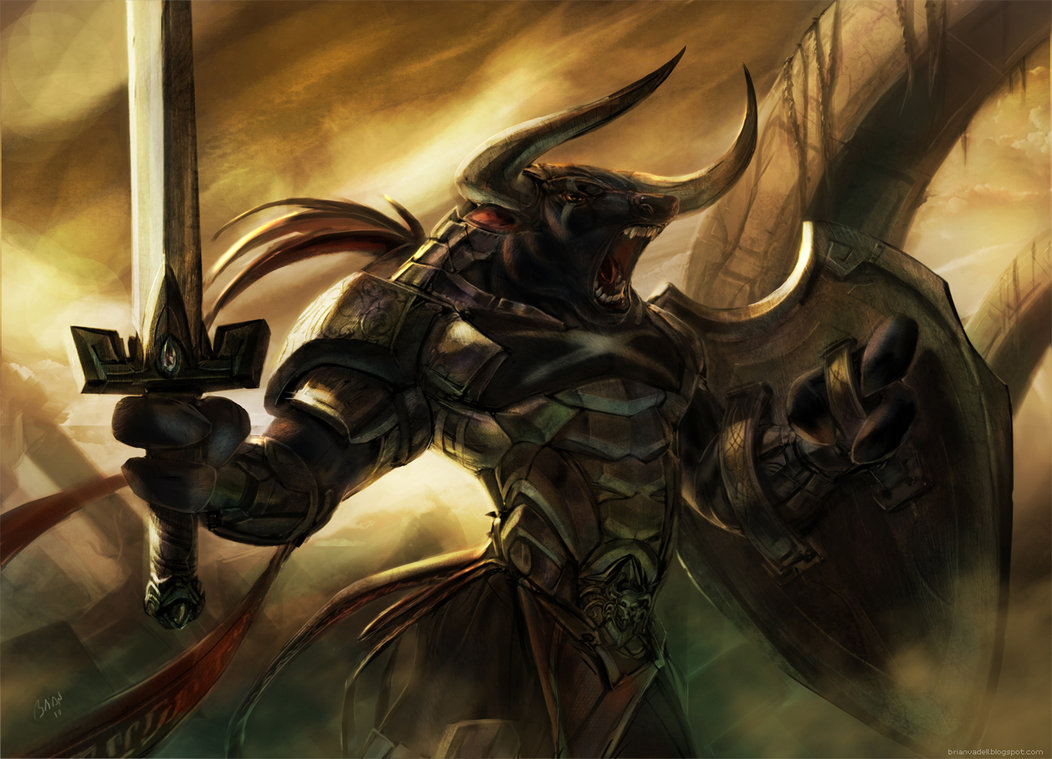
\includegraphics[width=\columnwidth]{minotaur_by_brianvadell}
%\end{figure}

\section{Midgaardian Spymaster} 
\section{Midgaardian Crusader}
\section{Midgaardian Knight Errant}
\section{Brouliard Cavalier}
\section{Brouliard Courtier}
\section{Brouliard Musketeer}
\section{Nessian Vikingr} This is an unusual class in that it is a combination of raider, trader and farmer. This is a hybrid class that aims to capture the realities and vicious myths of the vikingr people. 
\section{Nessian Ranger of the Black Thumb}
\section{Abloni Gladiator} A fearless warrior who is a master of melee combat (to the exclusion of other forms of combat). Uses a theatrical style of fighting that makes it very hard to use in massed formations (balancing aspect).
\section{Abloni Legionnaire Mercenary} A phalanx fighter whom is also a skilled manual labouring engineer (skilled in building quick fortifications, walls, roads, watch towers).
\section{Abyssian Witch Doctor} Known to the people of the Old Empire as a Witch Doctor, in fact the opposite is the case. The people of Abyssimiar have a more advanced understanding of medicine than than their ex-imperial cousins. From the perspective of the peasant however they are mystical and esoteric healers. 
\section{Abyssian Chariot Archer} 
A master of bow, spear and throwing axe. They are excellent at riding a Chariot. The class comes with a Loyal Henchmen whom fights with them. In exchange for the lack of normal henchmen, the class comes with other benefits.
\section{Venturer}

\newpage
\chapter{Backgrounds}\label{backgrounds}


\section{Social Class} The social class system is deeply entrenched in the world and has a fundamental influence on the character's upbringings. The nature of what each social class represents differs from Kingdom to Kingdom. Loosely however there are categories which can be classified. This book does not intend to go into detail on how each Kingdom's social class is like.

A nice example of this point though is that in Abyssimiar the warrior class are part of the lower social classes, whereas in Midgaard the warrior class would more likely be in the middle social classes, whereas in Brouliard they are more likely to be in the Lower Upper Class.

\begin{itemize}
    \item Upper Upper Class (UUC)
    \item Middle Upper Class (MUC)
    \item Lower Upper Class (LUC)
    \item Upper Middle Class (UMC)
    \item Middle Middle Class (MMC)
    \item Lower Middle Class (LMC)
    \item Upper Lower Class (ULC)
    \item Middle Lower Class (MLC)
    \item Lower Lower Class (LLC)
\end{itemize}

\section{Family}
\paragraph{How did your parents treat you?} Good, Okay, Bad.
\paragraph{How many siblings do you have?} 1-9
\paragraph{What are your relationships with them like?} Good, Bad
\paragraph{Was you firstborn or what?} No, Yes, ...
\paragraph{What is the situation with your family?} Good, Bad, Terrible, Glorious, Damned

\chapter{Feats}\label{feats}

There are two basic types of feats. Those that are general and can be taken by anybody, and those that are race specific with the intent on emphasising the unique look and feel that the race contributes to that characters identity. 

\begin{framed}\centering
        On Feat Design. The best kind of feats are those that have really interesting and deep gameplay effects. They should aim to add delicious flavour to the character. They should not rely heavily on some numbers in like +1 in order to deliver impact. 

They do not necessarily have to be mechanical buffs, or even balanced. Some feats are intended to provide players an additional way to make the game for challenging for themselves specifically. Feats that have a fundamental influence on the strategy of a character are also greatly desired as well. 

Feats such as Scholarly Skepticism are designed with the narrative in mind, and they help empower the character to shape the flow of the story. It is thus an explicit declaration to the GM and other players about your character.

The ramification of these design principles can be seen below.           
    \end{framed}

\subsection{General}
    \paragraph{Dead Man Walking} You are living on borrowed time. Do what thou wilt. 
    \paragraph{Haunted} You believe that the spirit of an ally, close friend or something has come back from the grave and now acts as your guardian. This could be a good thing, but it might not be.
    \paragraph{Jaded}
    \paragraph{Redhead} According to folklore, some people born with red hair are marked by the fey. You are one such person. 
    \paragraph{Reincarnated} You have vague, dream-like memories of a past life. You might even possess skills that you never knowingly learned.
    \paragraph{Coward} Upon reaching 40\% of your current health, you automatically flee as soon as possible.
    \paragraph{Hardened Criminal}
    \paragraph{Seasoned Traveller} This feat can be gained for free by sufficiently exploring the world. 
    \paragraph{University Education}
    \paragraph{Albino}
    \paragraph{Machiavellian} You have a silver tongue and a natural presence about you. You have learned to put this innate charm to use as a political predator. 
    \paragraph{Vampirism} Your max health is halved. In exchange, you can lifesteal.
    \paragraph{Scholarly Skepticism} You possess a keen logical mind and put faith only in your rationality and observation. 
    \paragraph{Portents} You are blessed (or cursed) with hazy visions of the near future. These take the form of vague feelings of comfort or dread that manifest on the cusp of pivotal choices. 
    \paragraph{Smitten} You are truly and deeply in love, in the purest storybook sense. Your love is not necessarily requited, but acts as a source of strength and purpose, for you would cross oceans and mountains to protect your beloved. 
    \paragraph{Military Veteran}
    \paragraph{Damned} For some reason a God has marked you down as undesirable. The reason is up to you. 
    \paragraph{Innocent}
    \paragraph{Unyielding Devotion} So firm are you in your crusade that your mind is nearly unassailable by those who would end it. Your faith literally dominates your life. Heresy hits you with feelings of rage and indignation, compelling you to ruthlessly stamp it out. So strong is your belief in the righteousness of your struggle that you inspire others by your example. 
    \paragraph{Paranoid} Self explanatory. Sometimes your belief might be unfounded or exaggerated. But those odd times when you are right, you will be glad you are a paranoid bastard.
    \paragraph{Forsaken Thoughts} The origin of the meditations of the Forsaken Thoughts is shrouded in secrecy. No warrior has ever admitted to knowing them, for the techniques were said to involve rejecting the Divine in all its forms.
\subsection{Flaws}
    \paragraph{Near-sighted} Things far away seem blurry.
    \paragraph{Braggart} You tend to EXAGGERATE!
    \paragraph{Eidetic Memory} You tend to remember things with absolute clerity.
    \paragraph{Alzheimers} You have trouble remembering where you are. You are not allowed to use any maps.
    \paragraph{Know No Pain} You dont know your HP. 
    \paragraph{Tunnel Vision} You often lack peripheral vision. 
    \begin{figure}[h]
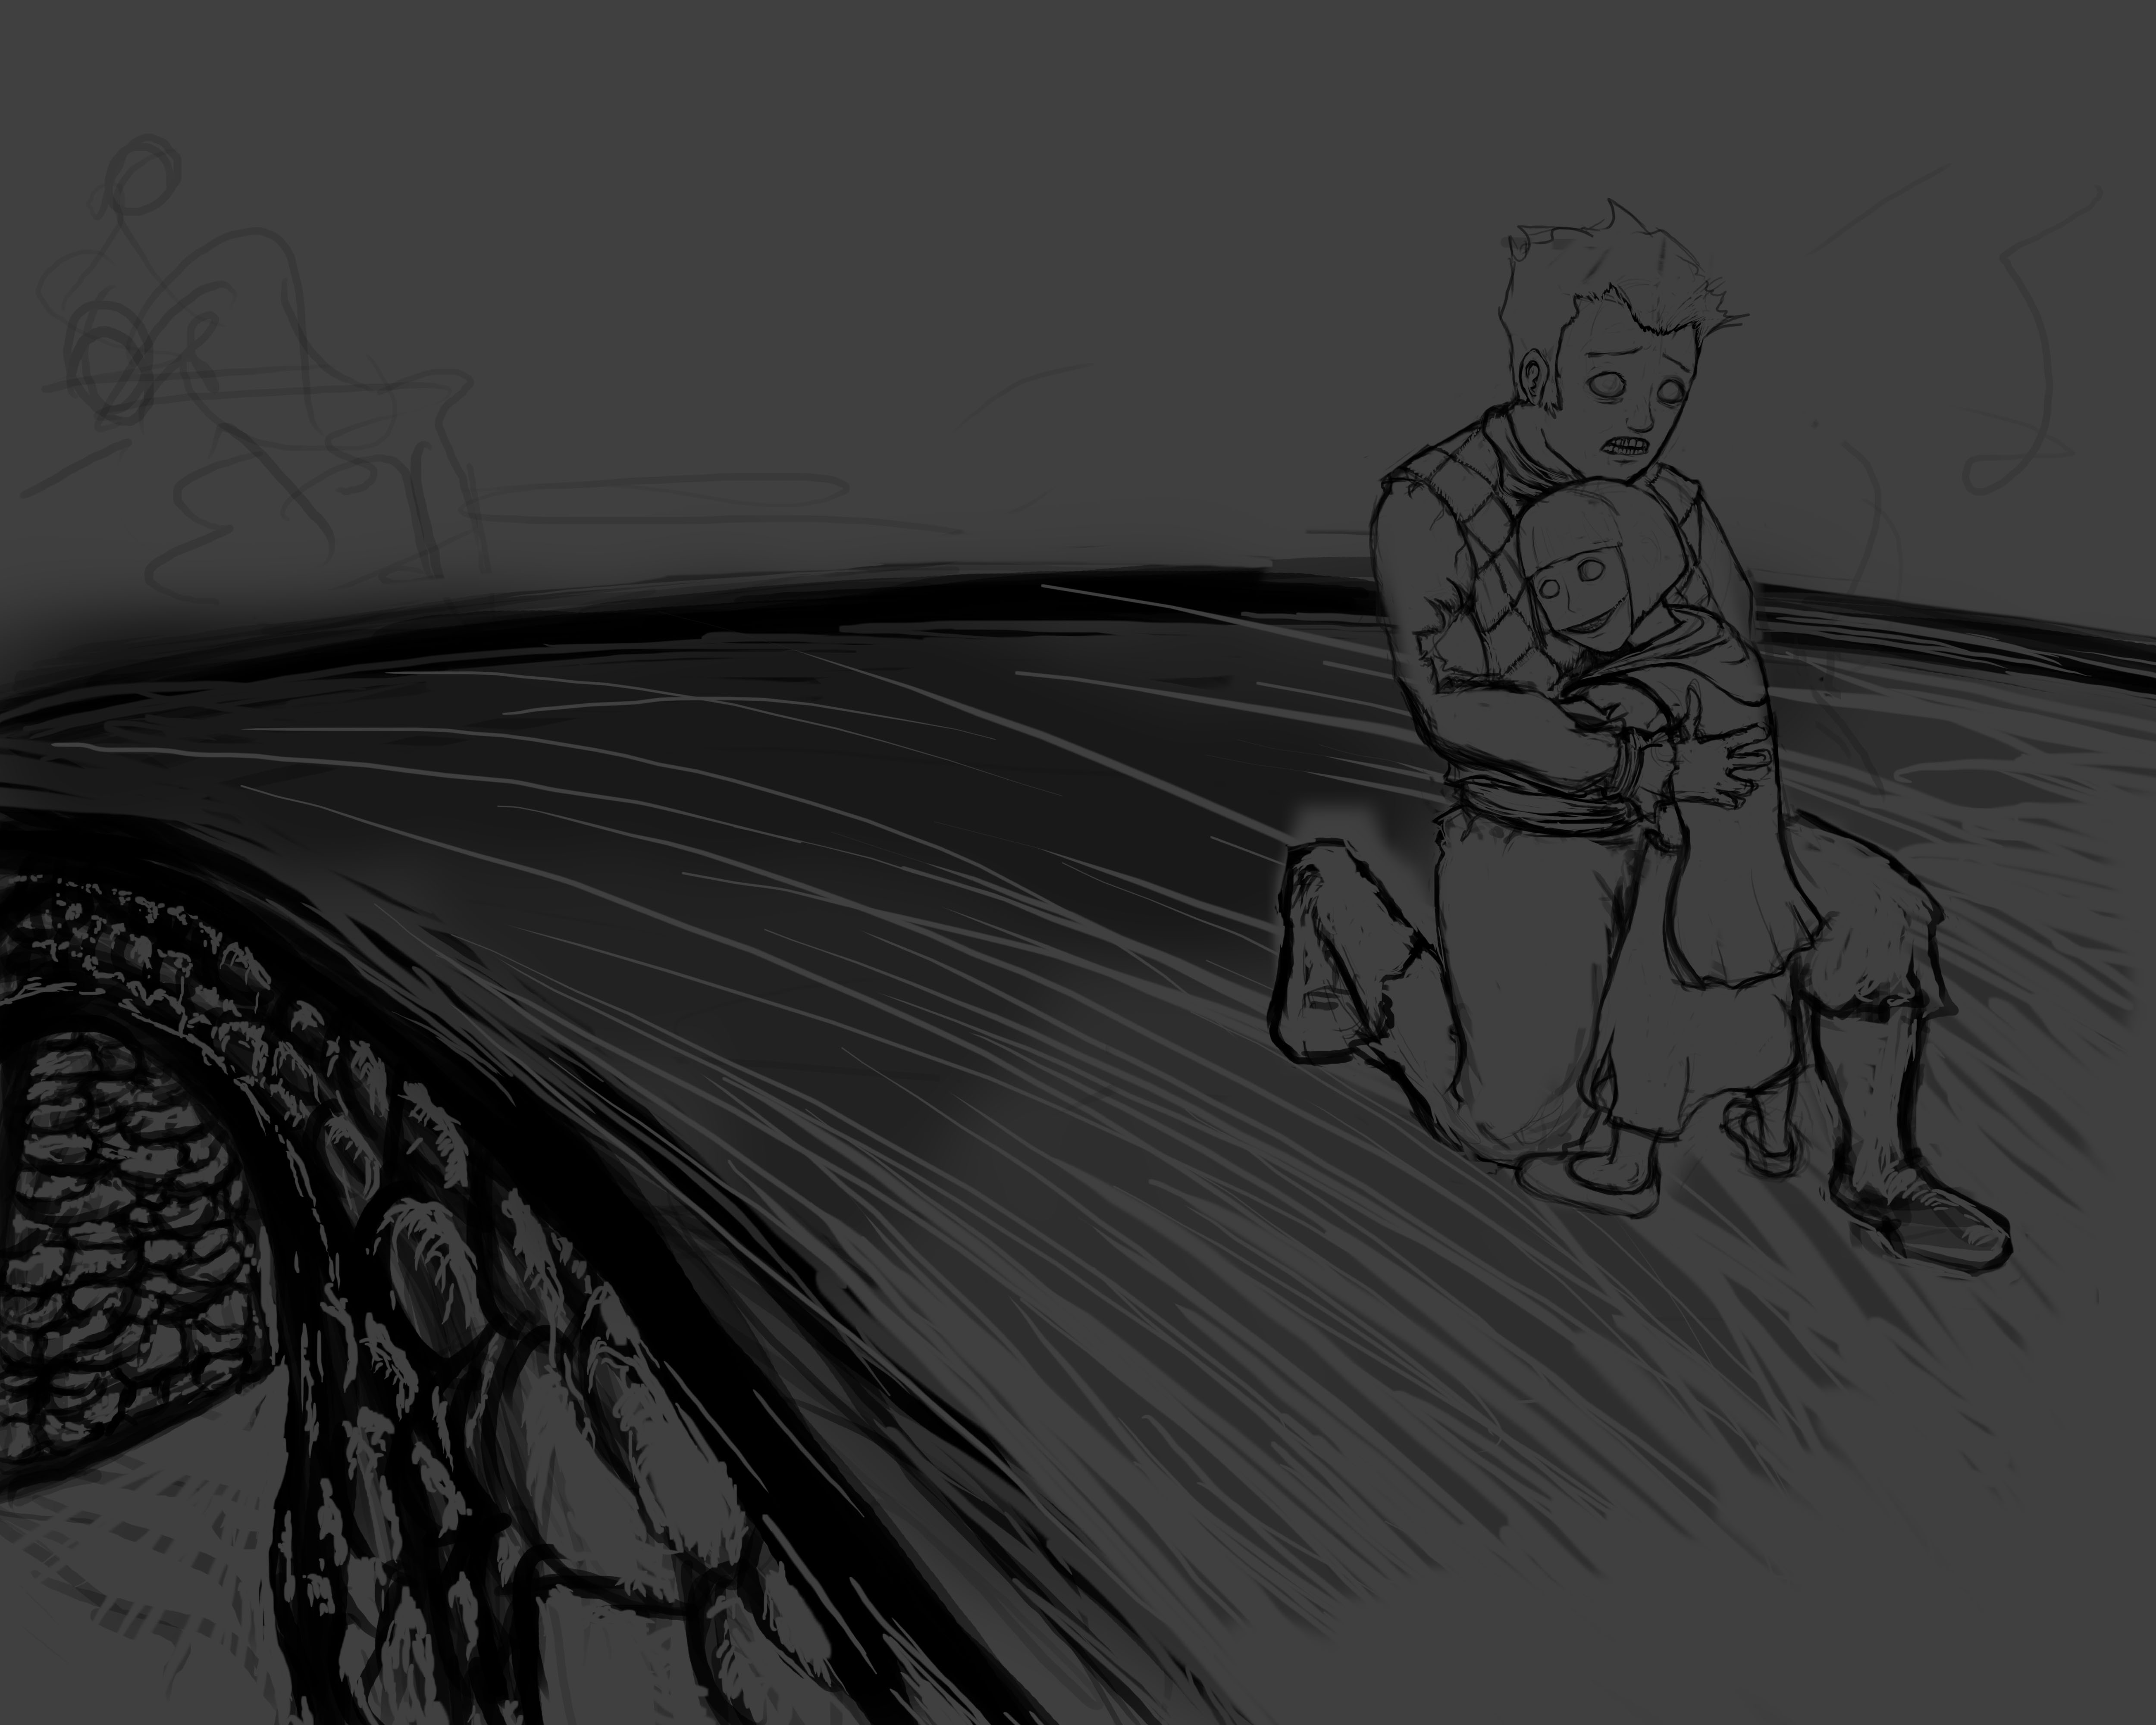
\includegraphics[width=\columnwidth]{rakaarth4}
\end{figure}
\subsection{Racial - Fire Giant}
    \paragraph{Heart of Fire} You are immune to any form of fire damage.
    \paragraph{Door Smasher} You can smash down a wooden door in a single round (6 seconds). 
\subsection{Racial - Gnoll}
    \paragraph{Refuse Eater} You gain sustenance from, and are resilient to, foods that would be considered disgusting by other Races standards. 
    \paragraph{The Hunt} Gnolls with this feat are the best at punishing foes who flee a close quarter engagement. I suggest allowing for a free attack.    
\subsection{Racial - Human}
    \paragraph{Outlander} You are literally not from this world. Outlanders simply appear in the wilderness with no gear at all. Unless an outlander actively aims to culturally immerse themselves they always seem to be foreign to the locals - in part because of their appearance, mannerisms, accent and behaviour. Except in the most cosmopolitan of areas, Outlanders are seen with at least suspicion, if not worse.
\subsection{Racial - Wood Elves}
    \paragraph{Woodland Traveller} Forest type terrain causes you no movement penalties.
    \paragraph{Squirrel} Fleeing a close quarter engagement is much less dangerous for you.
    \paragraph{At Peace with Nature} All natural wildlife are passive towards you and begin with the neutral mentality. One consequence of this is that even the most cowardly of animals will not flee on discovering your presence. 
    \begin{framed}\centering
        The Gnoll race are the best Hunters and the Wood Elf race are the best at escaping combat. Both their racial feats cancel each other out - and thus fleeing and chasing is as normal. Thus, they counter each other in a sense.          
    \end{framed}
\subsection{Racial - Dark Elf}
    \paragraph{Improved Infravision} Doubles infravision range to 120ft.
    \paragraph{Climb Steep Surfaces} They can climb as a rogue. If they are a rogue, they climb twice as fast as normal. A consequence of this is that Dark Elves are capable of taking advantage of certain terrain in ways that other races are simply not capable of doing so.
\subsection{Racial - Dwarf}
    \paragraph{Unyielding before Death} Dwarves whom reach the state when others die instead get forced into a catatonic coma state. This occurs unless the Dwarf dies to massive damage. If the Dwarf suffer further damage - such as being executed - they will die. After a time period, such as 1 week, the Dwarf will recover to 0 hp.  
    \paragraph{Dwarven Vigor} You heal health at twice the normal rate. 
    \paragraph{Vengeance Seeker} It is a terrible idea to wrong a Dwarf for they have deep memories, long lifespans, and a thirst for vengeance that eclipses most men. Dwarves are capable of memorising the faces of those whom wronged them to the most minute detail - an almost picture perfect memory - and this image haunts them till the day they die. A consequence of this is that it aids the Dwarf in hunting down those whom have provoked their wrath. 
\subsection{Racial - Gnome} 
    \paragraph{Family Connections}
\subsection{Racial - Half Elf} 
    \paragraph{Stars in the Night Sky} Many Half Elves are extremely extroverted, and more than any other race capable of building and developing relationships and reputations with people. Half Elves are allowed one additional Henchmen above what is ordinarily allowed just due to their force of personality. Additionally, once per day when dealing with any problem, a Half Elf may declare that they know someone who could help the players in this problem; it is upto the players and the GM to determine who could feasibly help, and importantly, how will they know and how will they get there. 

\chapter{Cosmology}\label{cosmology}
\pagecolor{gray}\afterpage{\nopagecolor}
\newpage
blah blah blah
\pagecolor{gray}\afterpage{\nopagecolor}
\fontfamily{pzc}
\selectfont

\newpage
\normalfont
\changepage{9cm}{9.4cm}{-4.7cm}{-4.7cm}{}{-4.5cm}{}{}{}
%\noindent\rule{\textwidth}{\textheight}
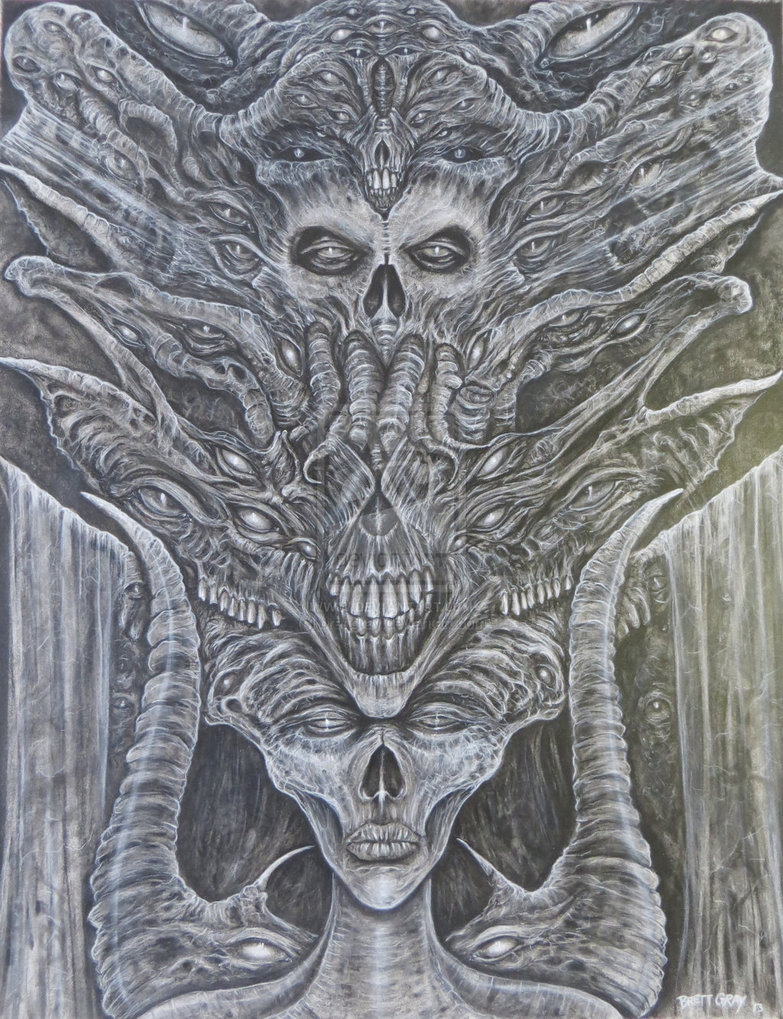
\includegraphics[width=\textwidth,height=\textheight]{priestess}
\newpage

%restoring the standard settings
\changepage{-9cm}{-9.4cm}{4.7cm}{4.7cm}{}{4.5cm}{}{}{}

\section{Creation Myths} In the beginning there was the void. Without warning came thought, unattached ambiguous thought. This thought soon grew and spawned the first light. From light came the memory of the dark and from that memory thought grew and created the world and the heavens. From the earth humans and animals grew. Men and animals had their own thoughts as well and this eventually spawned differences. These differences spawned women and different species. These differences created hatred and love, and from that strength and weakness, predator and the prey.

Communities formed to protect one from another and soon war. The conflict spawned more complex thoughts and questions. Soon the Gods were imagined and like all before, the Gods were different from one another. Gods ruled all the lesser beings and also warring with one another. These wars ravaged the world; civilizations grew from the conflict only to fall only to be replaced by newer and greater ones. The Gods depend on the conviction of their followers and as followers fall in these wars, Gods disappear, forgotten.

Humans became the dominate species and created technological wonders that replaced many Gods. The other species found comfort in lands humans would not claim. Some Gods who felt their time was at an end created Gates for them and their followers to retreat through. These Gates served as their ultimate refuge to the world, and lead them to a new world. As only three Gods remained, and would later be known as The Lords of Ends. Wars became more common. Communities were shattered; families butchered one another for little or no reason. Finally the greatest of all factions created a weapon that one ends all wars, all that ended was civilization.

With the world ravaged, the surviving creatures are left alone once again. None of survivors wished to remember the Lords of Ends and soon these Gods also died. One human dedicated himself to studying the lost arts and in time developed once forbidden arts. He mastered once forgotten arts of the old world and mastered all schools of magic. His students worshiped him and his power grew stronger and became the first human to truly ascend to that of godhood. He soon discovered the Gates and opened them. Some opened up violent worlds with even more violent and angry gods. Conflict began a new and the Gods returned to a new world and brought forth a new age.

%\begin{framed}\centering
% What you have here is a pantheon of recurring "pseudomythological" entities and a collection of arcane books that supposedly yield insights into the mythology.
% \end{framed}

\newpage
\section{Haeckel Pantheon}

\begin{tabular}{l | p {8 cm} | l}
    Deity & Domains & Worship Centers \\
    \hline
    \hline
    Aratron & Knowledge, Memory, Thought, Imagination, Magic, Arcane, Divine, Rune, Language, Wards & \\
    \hline
    Junon & Community, Family, Home, Judgement, Divine, Light, Stars, Knowledge, Moon & Midgaard \\
    \hline
    Alesia & Charm, Love, Lust, Family, Community, Law, Tyranny, Slavery, Revelry & \\
    \hline
    Gigas & Law, Loyalty, Nobility, Judgement, Leadership, Glory, Honour, Heroism, Strength, Resolve, Tactics & Ablon \\
    \hline
    The Priest King & Good, Redemption, Healing, Restoration, Resurrection, Judgement, Divine, Matyr, Purity, Protection, Community, Revelation & Midgaard\\
    \hline
    The Dyad & Charm, Love, Lust, Family, Cooperation, Loyalty & Brouliard \\
    \hline
    Ma'asei & Heroism, Glory, Honour, Inevitable, Explorer, Resolve & Ubris Furor \\
    \hline
    Magnus, Dante & & \\
    Secretum & & \\
    Nostra & & \\
    Mewgner & & \\
    The Hanged Man & & Nosquam \\
    Charon & & North Wall\\
    Sich & & \\
    Ra Herakht & & Abyssimiar \\
    Tinu & & \\
    Phex Eris & & Avalonia \\
    Waddell & & \\
    Neyord & & \\
    Asint & & \\
    Ignis & & \\
    Janus Thurinus & & South Midgaard \\
\end{tabular}


\begin{multicols}{2}
\subsection{Aratron} Master of the Divine, Lord of Aether, Master of all Mysteries, Divine Immanence.

Born a human and ascended to Godhood. Aratron is one of the survivors of the first world. He spent the last years as a mortal studying the lost arts of the old world and eventually developed the arts of Magic. His wisdom and power became so great that it propelled him to that of the Gods. He quickly grew lonely and curious as to the fate of the old Gods. This curiosity leads of to the Gates which the old Gods stepped through to avoid the coming disaster which ended the First World. He then opened all the Gates, returning all the exiled Gods and their followers to the New World.

Aratron is often associated with the God Nostra, whom travel through all seven Gates. Followers of both beliefs will often help one another and very rarely quarrel. Some of his followers argue with whether they should seek to be as Aratron and gain more power, or if such a task will anger the God and see such a task as a challenge.

The Church of Aratron tasks itself with preserving knowledge and perusing mystical arts. Certain sects aim to emulate their God and attempt to ascend to the heavens themselves, while others believe their God survived as a warning and that great power must be kept under control lest the world remakes itself yet again. The institution itself holds the later view, regulating magic users across Haeckel and even providing shelter to those who are hunted by mage slayers. A number of territories will respect such refuges out of fear of the Church's wraith. The Church however has never shown an act of aggression on non magic users. Many of these Churches can be found amongst universities, for they serve more as schools rather than places of worship.

Aratron is often depicted as wearing a white robe with a red cape. In his right hand is a wand raised towards the heaven, while his left hand is pointing to the earth. This gesture has multiple meanings, but is endemic to the Mysteries, symbolizing divine immanence, the ability of the magician to bridge the gap between heaven and earth. A table is often shown to be in front of Aratorn, on the table are the symbols that signify the classical elements of earth, air, fire and water. Beneath are roses and lilies changed into garden flowers, to show the culture of aspiration or symbolizing that he existed when the world was made anew.

Head masters of Aratron's flock will adorn a White robe covered by a red cape. The clothes that Aratron is often depicted wearing. Emissaries of Aratron are often highly coveted by those seeking great power.

Followers of Araton believe any book containing the knowledge of magic to be Holy Text. There are two books that are said to have been written by Aratron, one being The Gospel Vermillion and The Grammatica Aratron.

It is said that The Gospel Vermillion is was written with the blood of those who died from the First World and that it contained locations and designs of lost relics of power and that the pages have been scattered. The Grammatica Aratron is said to contain every spell that can ever be known and that these pages have also been scattered.

Although there is no religious holiday there is one day a year in which the Church of Aratron opens its doors to a new neophyte and announces a new Adept.

\subsection{Junon} The Holy Mother, Holy Mother Church

\subsection{Alesia} Queen of the Gods, Goddess of Beautiful things, Goddess of Abundance, Mother of A Thousand

\subsection{Gigas} Emperor of the Gods, The All Father, Caesar Dominus

\subsection{The Priest King} The mortal representative of the Gods

\subsection{The Dyad} The Lovers, The Holy Couple, The Inseparable Two

\subsection{Ma'asei}

\subsection{Magnus, Dante} 

\subsection{Secretum}

\subsection{Nostra}

\subsection{Mewgner}

\subsection{The Hanged Man}

\subsection{Charon}

\subsection{Sich}

\subsection{Sanat}

\subsection{Ra Herakht}

\subsection{Tinu}

\subsection{Phex Eris} 

\subsection{Waddell}

\subsection{Neyord}

\subsection{Asint}

\subsection{Ignis}

\subsection{Janus Thurinus}

\end{multicols}

\section{Abyssimiar Pantheon}

\newpage
\section{The Seven Major Cosmologies of Haeckel}
\begin{multicols}{2}

Within Haeckel there is no defined cosmology that is 100\% correct. Scholars from all around the Known World agree or disagree on the topic. The Magic systems themselves are known to contradict each other - with most Magi's spells following their own personal theories. 

\subsection{Ptolemaic Model} Universe orbits about a stationary Oerth. Planets move in circular epicycles, each having a center that moved in a larger circular orbit (called an eccentric or a deferent) around a center-point near the Earth. The use of equants added another level of complexity and allowed astronomers to predict the positions of the planets. The most successful universe model of all time, using the criterion of longevity. It is also known as the Great System, its theoretical foundations written by the Scholar Almagest. Classification: geocentric, abyssimiar. 
\subsection{Medieval Philosophy} A universe that is finite in time and has a beginning proposed by Philosopher Philoponus who argues against the ancient notion of an infinite universe. Since then further logical arguments supporting it have been developed by philosophers and theologians in Midgaard.

\subsection{Cartesian Vortex} A system of huge swirling whirlpools of aethereal or fine matter produces what we would call gravitational effects. His vacuum was not empty. All space was filled with matter that swirled around in large and small vortices. Classification: Static (evolving), steady state, infinite, renaissance.
\subsection{Memonaic Central Fire} At the center of the Universe is a central fire, around which Oerth, Sun, Moon and planets revolve uniformly. The Sun revolves around the central fire once a year, the stars are immobile. The earth in its motion maintains the same hidden face towards the central fire, hence it is never seen. This is the first known non-geocentric model of the Universe. This model was first proposed by the Firegiant Stargazer Memonaic. Classification: pythagorean, ancient.
\subsection{Cyclic Oscillation} One cycle of existence is around 3000 years and the life of one universe around a million years. This Universal cycle is preceded by an infinite number of universes and to be followed by another infinite number of universes. Includes an infinite number of universes at one given time. Central to this belief is the notion of the everlasting soul that reincarnates its self with each cycle; thus the pool of souls in reality never changes in number.
\subsection{Celestial Sphere} Spherical earth is surrounded by concentric celestial spheres. Universe exists unchanged throughout eternity. Contains a fifth element, called aether (later known as quintessence in Brouliard), added to the four Classical elements. This model is deemed heretical in Midgaard.

\subsection{Absolute Time and Space theorum} According to Magi Arakaban, absolute time exists independently of any perceiver and progresses at a consistent pace throughout the universe. Unlike relative time, Arakaban believed absolute time was imperceptible and could only be understood mathematically. According to Arakaban, humans are only capable of perceiving relative time, which is a measurement of perceivable objects in motion (like the moon or sun). From these movements, we infer the passage of time. These notions imply that absolute space and time do not depend upon physical events, but are a backdrop or stage setting within which physical phenomena occur.

\end{multicols}

\chapter{Equipment}\label{equipment}
\pagecolor{gray}\afterpage{\nopagecolor}
\newpage
\pagecolor{gray}\afterpage{\nopagecolor}
\fontfamily{pzc}
\selectfont
In the Midgaardian Keep, Castle Black, a young noble Lord aged 11 lays in bed. His servant, a short lady who has seen many years sits in a chair on the opposite side of the room. She knitts a scarf with delicate and refined movements. 

``Have I ever told you that my pappy fought in the Great War? It was a long time ago, your parents had'nt even been born yet.''

``I dont like those kind of stories. Knights in shining armour are not my thing.''

She chuckles, ``So what kind of stories do you like my little Lord.''

``The scary ones.''

``The Great War was scary my little Lord! It wasn't a romance tale like your sages say. 'The Days of Dread' - that's what we called life back then. There were no goodly kings then, no no. One House was composed of vile necromancers!''

``The Mordenheims? I read a bit of them, but my teachers constantly change the topic when I inquire further.''

``We didn't know them by their names then, young Lord, but we knew what they did. Long after the war had ended, Pappy would wake up in the night sometimes screaming. When I was grown I finally asked him why that happened, and he said: 'Every time I sleep I see my brother. But not... like you knew him, Helga. I see him when he was killed. And I see him when he rose again, and I see him when he tried to strangle me with his cold, dead hands. And finally, I see his walking corpse's head sliced clean off by my commander.' ''

The little Lord rests his head on his silk pillow. On his fair and normally jaded face curls a small smile. 

\normalfont
\newpage



\section{Simple Exploration Logistics}

\begin{tabular}{l l l l l }
    Type & Desc & Lasts & Cost & Weight \\
    \hline
    A & Basic Excursion & 3 days & 25 gp & 30lb \\
    B & Extended Excursion & 7 days & 50 gp & 75lb \\
    C & Prolonged Excursion & 14 days & 120gp & 140lb \\
    D & Basic Dungeon Crawl & 1 day & 50 gp & 50lb \\
    E & Extended Dungeon Crawl & 3 days & 100 gp & 85lb \\
    F & Basic Overland Excursion & 2 days & 35 gp & 50lb \\
    G & Extended Overland Excursion & 7 days & 80 gp & 100lb \\
\end{tabular}

\begin{framed}\centering
The purpose of this system is for campaigns where resource management or the specific use of inventory items is simply a distraction and is heavily de-emphasised in that scenario. For verisimilitude purposes you can say that due to wear and tear the items in the kit simply are heavily damaged, muddy beyond use, or whatever.  
\end{framed}
\begin{multicols}{2}
\section{Starting Equipment Sets}

\subsection{Brouliard}

\paragraph{Socialite} Small dog familiar, long slender sword, stiletto, form-fitting chain mail armor, silvery white silk cloak and sapphire blue dress, tear-drop silver earrings (10gp value), high boots, 2 purses, 1 week’s iron rations, 31gp

\paragraph{Dilettante} Slightly notched short sword, dagger, leather armor, shabby linen tunic and pants, leather belt, low boots, belt pouch, pair of dice carved with leaves, 1 week’s iron rations, 3gp

\paragraph{Intriguer} Composite bow, quiver with 20 arrows, long slender sword, stiletto, light steel shield, form-fitting chain mail armor, midnight blue cloak embroidered with silvery, midnight blue cassock, high boots, backpack, 34gp.

\paragraph{Swashbuckler} Shortbow, quiver with 20 arrows, scimitar, 2 well-balanced daggers with boot- sheathes, leather armor, colorful tunic and pants, bright silk girdle, high boots, wineskin with good wine, small sack, 50' rope, grappling hook, 1 week’s iron rations, 7gp.

\paragraph{Aristocrat} Crossbow, case with 20 bolts, matching sword and dagger with lacquered hilts, exquisitely stitched leather armor, fur-lined cloak, armiger’s tunic and pants, embossed leather belt, high boots, medium riding horse, riding saddle and tack, saddlebags, 1 week’s iron rations, 20gp

\paragraph{Bounty Hunter} Bola, serrated sword, dagger, net, leather armor, black cloak, traveler’s tunic and pants, high boots, backpack, crowbar, 50' rope, manacles, 12 iron spikes, small hammer, 2 weeks’ iron rations, 2gp.

\paragraph{Cutthroat} Hand axe, dagger, leather armor, cheap tunic and pants, leather belt, low boots, backpack, 12 iron spikes, small hammer, 1 flask of military oil, tinderbox, 12 torches, 2 weeks’ iron rations

\paragraph{Merchant Traveller} Crossbow, case with 20 bolts, short sword, 2 throwing daggers, sturdy leather armor, tanned brown cloak, thick tunic and pants, leather belt, low boots, backpack, 2 large treasure sacks, 50' rope, tinderbox, lantern, small hammer, 12 iron spikes, 2 flasks of military oil, wineskin, 2 weeks’ iron rations, 3gp

\paragraph{Nessian Vikingr} Bearded Longaxe, painted wooden shield, woolen cloak, iron helmet, NOT COMPLETE. 

\subsection{General} 
\paragraph{Abloni Free Gladiator} Gilded sword, large steel shield, lamellar armor, plumed heavy helmet with visor and crest, leather cloak, loincloth, high sandals, backpack, amphora of oil (for polishing body), 2 weeks’ iron rations, 15gp in arena winnings

\paragraph{Hunter} Sturdy longbow, quiver with 20 arrows, leaf- headed spear, gracefully curved short sword, dagger, chain mail armor, wind-battered fur cloak, wool tunic and pants, leather belt, low boots, backpack, lantern, tinderbox, 2 flasks of common oil, blanket, 50' rope, 12 iron spikes, small hammer, wineskin, 1 week’s iron rations

\paragraph{North Wall Death Dealer} Two-handed iron sword, francisca, chain mail armor, wool tunic and pants, leather belt,
low boots, silver arm-bands (25gp value), wineskin with strong ale, small sack, 50' rope, grappling hook, 2 weeks’ iron rations, 1gp

\section{Equipment Kits} 

\begin{framed}\centering
The purpose of these are to speed up the purchasing process as well as making it obvious to new players the kinds of items they will need.  
\end{framed}

\paragraph{Kit, Infiltration; Price 140 gp; Weight 15 lbs;}

This kit is useful to adventurers who must practice guile and deception in order to acquire useful information, and includes a set of caltrops, chalk, a disguise kit, an ear trumpet, fake footprint shoes, a skeleton key, and a wrist sheath. For Small creatures, the weight of an infiltration kit is 9 pounds.

\paragraph{Kit, Gear Maintenance Price 5 gp; Weight 2 lbs.}
This kit contains metal polish, a small file, a leather paring knife, conditioning oil for leather, two soft cloths, extra leather straps, a sewing needle, and a few buttons.

\paragraph{Kit, Grooming; Price 1 gp; Weight 2 lbs.}
This pouch of toiletries includes a comb, scissors, a nail file, a sponge, a hairbrush, a miniature mirror, soap, a chewing stick, and tooth powder.

\paragraph{Kit, Fighter's; Price 9 gp; Weight 29 lbs.}
This kit includes a backpack, a bedroll, a belt pouch, a flint and steel, an iron pot, a mess kit, rope, soap, torches (10), trail rations (5 days), and a waterskin.

\paragraph{Kit, Cooking; Price 3 gp; Weight 16 lbs.}
This kit contains an iron pot, an iron skillet, a ladle, a skewer, a wooden cutting board, a cutting knife, an iron tripod for the pot, a packet of tinder, and a small selection of local or otherwise easy to find seasonings. You can attach the skewer to the tripod for roasting small game animals. All the component pieces (except the skillet) fit within the pot for easy storage and transport.

\paragraph{Kit, Cleric's; Price 16 gp; Weight 32 lbs.}
This includes a backpack, a bedroll, a belt pouch, candles (10), a cheap holy text, a flint and steel, an iron pot, a mess kit, rope, soap, a spell component pouch, torches (10), trail rations (5 days), a waterskin, and a wooden holy symbol.

\paragraph{Kit, Campsite; Price 12 gp; Weight 80 lbs.}
This kit is actually four bundles of gear, designed so four individuals can share the load. It consists of four bedrolls, four blankets, a day's worth of firewood, a flint and steel, a tindertwig, four mess kits, a cooking kit, and 8 days of trail rations (with the expectation that adventurers will supplement the rations with a little hunting as they travel). Adventurers expecting inclement weather should also purchase one or more tents.

\paragraph{Kit, Breaker's; Price 353 gp; Weight 40 lbs.}
This kit contains all manner of items useful for smashing down doors, creating diversions, and blowing things up. It includes a dose of alchemist's glue, a flask of alchemist's fire, a crowbar, a drill, a fuse grenade, a glass cutter, a jetcaster, a vial of phosphorescent gel, 4 pints of oil, a portable ram, a dose of rusting powder, 5 tindertwigs, and a wire.

\paragraph{Kit, Riding; Price: 16gp; Weight 54 lbs.}
This kit includes a bit and bridle, a saddle, a saddle blanket, saddlebags, and 2 days' worth of feed for a mount. The weight can be lightened 10 pounds by discarding the feed.

\paragraph{Kit, Rogue's; Price 50 gp; Weight 37 lbs.}
This kit includes a backpack, a bedroll, a belt pouch, caltrops, chalk (10), a flint and steel, a grappling hook, an iron pot, a mess kit, a mirror, pitons (10), rope, soap, thieves' tools, torches (10), trail rations (5 days), and a waterskin.

\paragraph{Kit, Gypsy Signal Kite}

Gypsies are a strange lot. Given that they travel and do not rely on societies messenger systems they have needed to develop their own way of communicating with each other. To this end they invented signal kites. Built from paper glued to bamboo frames, their kites are painted with various colors and pictures. In addition to flying kites as a leisure activity, gypsies also fly kites of various shades and patterns to send signal messages. Gypsies have developed an extensive code of signals and can use their kites to display complex messages visible at great distances. A signal kite kit includes six small colored kites that can be hooked together in different patterns to facilitate complex messages. The kit also includes a spool and 300 feet of twine. Sending or interpreting a signal kite's message requires understanding the Gypsy language.

\paragraph{Kit, Trapper's; Price 263 gp; Weight 90 lbs.}

This kit is particularly useful for dungeon explorers who specialize in trapping or taming whatever vile quarry they find. A trapper's kit contains an average lock, a bear trap, a container of bone paste, a Small cage, a set of manacles, a bag of marbles, 50 feet of silk rope, two tanglefoot bags, 50 feet of twine, and a wire.

% Marching
% Combat
% Infiltration
% Siege
% Encampment
% 

\end{multicols}

%\section{Fashion}
%\subsection{Ablon}
%\subsection{Abyssimiar}
%\subsection{Brouliard}
%\subsection{Midgaard}
%\subsection{Nes}
%\subsection{Ubris Furor} 

%\section{Design}
%Haeckel's vastness and social problems leads it to having differing levels of technological advancement from region to region. While Humanity dominate the continent it must be said that some of the most advanced technologies were in fact developed by demi-humans. As it currently stands, Elven and Dwarven Technology is superior to Humankind's; however the Megacity State of Ablon's technology is fast catching up and can be said to be superior in some regards. Most demi-human technology has been lost to the centuries, and what remains have their craftsmanship as closely guarded secrets that they would take to the grave. 
%
%\begin{framed}\centering
%Haeckel eschews the notion of wealth to level balancing. We have chosen to take this approach because it reduces the "resource optimisation problem" that you have in many systems. For example, if you give player's 20 points to spend on something, they will aim to allocate it efficiently. This is the problem that causes a lot of very interesting magical items to rarely be used - because wealth is a limited resource that is literally capped to ones level. You break that coupling and you open up new possibilities.
%\end{framed}
%\section{Gear Sets}
%
%The purpose of this section is to speed up character creation and the purchasing of large bulks of items by creating packages that players can rapidly pick to suit their various purposes. 
%
%\section{Potions}
%efefef
%\section{Scrolls}
%    \paragraph{Scroll of Magic Mapping} Scrolls of magic mapping are Scrolls that, when read, reveal part of or the entire level map (if blessed) to the player.\section{Books}
%    \begin{snugshade} "Spacing between words did not exist until the 7th century. This facilitated reading for monks who were not familiar with High Gothic. However, the use of spaces between words did not become commonplace before the 12th century. It has been argued that the use of spacing between words shows the transition from semi-vocalized reading into silent reading." -- Codex of Old Literature by Julius Toronicus. \end{snugshade}
%    
%    \subsection{Tome} A tome is a large book, especially one volume of a multi-volume scholarly work.
%        \paragraph{Summa Theologica} An Ancient Tome on the subject of Midgaardian Theology. It is one of the classics of Haeckel and one of the most influential works in that region. It is a major work and a lofty read at 3500 pages. The original text Summa Theologica Prime is considered a Holy Relic.
%    \subsection{Journal / Ledger}
%    \subsection{Codex / Tablet} Predominantely from Ablon.     
%    \subsection{Treatise}
%    \subsection{Papyrus Scroll} Predominantely from Abyssimiar and the Southern Continent.
%        \paragraph{The Creation Myth} 
%    \subsection{Atlas}
%        \paragraph{Atlas of the World} A rare and most visually compelling volume. Produced to the highest standards of the day by the leading mapmaker of the day. It is a clear, detailed, and intricate work of art. For each area there is an accompanying text, giving sources and authorities for them. It is a dense work and it takes awhile to read. 
%        
%        A sufficiently intelligent and literate character can use this book to, in a sense, ask the GM questions on the geography of the world. The answers do not have to be 100\% accurate but they are usually a good answer. To use this, it takes time (between 1-6 turns) to find the answer. The volume is heavy and thus cannot be easily carried onto adventures.  
%\section{Lighting}
%\section{Food}
%\section{Weapons}
%    \paragraph{Quick Dagger} This blade shimmers in a hyper active and accelerated matter. Legend speaks that it bestows upon the wielder amazing speed and alacrity. Thieves across the entire world covert this blade and very few of it exist.  
%\begin{framed}\centering
%This is the best known weapon for the Rogue class. The only way to get this blade is to steal it. Thus creates a shadowy conflict where treacherous individuals do whatever they can to acquire it and hold onto it long enough to profit highly from it.     
%\end{framed}        
%
%\paragraph{Bow of Light} Charges arrows with sacred light. The arrows will only harm those with evil in their heart. It will never harm those with good in their heart; the logical implication being that you can fire it safely at an opponent engaged in melee combat with a Paladin. The arrows charged with light emit it for a duration of 1 turn (10 minutes); thus it serves as a multi-purpose tool.
%
%\section{Armour}
%\section{Jewelry}
%\section{Wands}
%\section{Rods}
%\section{Staves}
%\section{Pets}
%\section{Navalcraft}
%\section{Tool}
%    \paragraph{Waterproof Blanket} Waterproof blankets will, while in the players' inventory, completely protect all inventory items from rusting and water damage. Note that worn items are not protected by waterproof blankets.
%    \paragraph{Hooded Cloak} Protects worn items from water damage - though not from full immersion in water. Thus, it would be effective vs heavy rain, but not vs a water trap or a flash flood. 
%
%\section{Unorganised}
%\paragraph{Prosthetic Limb}
%
%\paragraph{Mercy Giver} 
%\paragraph{Battle Gorget} This throat protector consists of a metal throat-shield and overlapping, neck-encircling plates that are attached to a leather belt. It protects the wearer from strangulation, death by hanging, and stabbing or piercing damage done directly to the throat. The voice of those whom wear this mask seems to echo and become a pitch rougher which makes them more intimidating.
%\paragraph{Bone Mask} This skull-face mask is fashioned from bone from any source – with the only limitation being that the pair that is created must be from the same litter of animals. The powdered bones of many animals can be used in a paste to augment or even form an entire mask. The mask can emit a spectral messenger once per day. This insubstantial magical construct looks like a skeletal bat and flies unerringly to the Bone Mask's pair.
%\paragraph{The Lumberjack's Axe} 
%\paragraph{Mind Twister} This artifact is a large (1-foot square) tome of raven black leather, embossed with a pattern of small grinning skulls and dark sunbursts against a twisting, warped background of torture and chaos. This book has golden hinges and clasps, and it is closed with a lock of unbreakable metal. The pages of this book are made of the flayed skins of the scribes of earlier, less-successful drafts of the tome. These interior pages are illuminated with strange, bestial designs imprinted on gold foil, and the text of the work is inscribed in bright red ink. Once begun, it is a hard book to put down. It is one of the most dangerous books on the continent. If it is read, the wearer is turned into a fanatical follower of a supernatural entity known as Abel Malouok. It takes the form of a demonic hydra made of blood drenched and blasting hot sand.
%\paragraph{Puffin Hound} The most ancient of Nessian breeds, this hound specialises at hunting seagulls, puffins and other sea birds. It has six developed toes on each foot. They can close their ear canals at will, and are able to bend their head 180 degrees backwards over their shoulders. Their legs are extremely flexible and can be stretched straight out to the side for greater ease in swimming or in maneuvering in narrow crevices in the sea-side cliffs where their avian prey lives. They are as expensive as a good milch cow, and can single handedly bring back upto 30 puffins in a single night. Puffins being a delicacy in Nes.
%
%Example names for Nessian Hounds: Gramr, Gifr, Garmr, Floki, Rosta, Samr, Saurr, Geri, Strutr, Surtr, Vala, and Vigi.
%
%\paragraph{The Inevitable} A crossbow with an exotic design. Each bolt fired from it is magically attached to a chain that hooks into the target. The target is then unable to escape as he is grappled unless he decides to wrip out the bolt (the chain is made of force and cant be broken by mundane weaponry). The crossbow provides a mechanism that allows the user to pull the victim towards the shooter.
%\paragraph{Dwarven Door Puncturer} A crossbow covered in dwarven runes. It fires crossbow bolts with such penetrating force that they are capable of going through wooden doors with ease – slicing through as if they're butter. The key drawback to the weapon is that it has half the effective range of a normal crossbow.
%\paragraph{Halberd of Vaulting} Magically enhances the user so that they're now capable of performing a powerful leaping attack. It provides a +30 on jumping checks and removes the usual jump distance maximums. Whenever the user takes a charge action they may perform this.
%\paragraph{Candle of Icy Death} This 1 foot tall 12 inches thick black candle is icy to touch. When lit, it burns a pale blue, gives off no smoke, it gives off no heat, and doesnt melt down. If examined with detect magic it radiates a necromantic aura. Every minute the candle is burning reduces the temperature by 1 degree in a 20 foot diameter until 0 degrees Fahrenheit is reached. Additionally, the candle prevents any healing – natural or magical, from occurring in its range. Once cast, the candle can only be snuffed by a bless spell. The temperature slowly returns to its normal temperature at the normal rate.
%\paragraph{Weightless Scabbard} It grows and shrinks to accommodate any bladed weapon. While in its scabbard, a weapon has its weight reduced to zero.
%\paragraph{Galeb Duhr Warhammer} The head of this massive warhammer is made of living rock. It was designed to destroy elves. It is an intelligent weapon that hates those who escape. As such, those who touch the warhammer (both those struck by the weapon, and those carrying it) have their moment speed reduced to half IF they try to escape. You are not even capable of making 5ft steps. This effect lasts for one hour.
%\paragraph{Tentacle Rod} Three long, russet coloured tentacles sprout from the end of this two foot rod, writhing simultaneously. The secret to crafting this horrible item was learned through nightmarish visions granted by the Eye – a mysterious and vile entity from the Dread Gate. The purpose of this device is completely unknown – nowadays cult leaders use this as a status symbol.
%\subsection{Elven Technology}
%
%\subsection{Dwarven Technology}
%
%\subsection{Nessian Magical Swords}
%A number of magical swords exist in the setting. However we have taken the approach that most are simply unknown, being so rare as to not be in the public's knowledge. There exists three magical swords that have taken on mythical proportions and are widely known in Nessian lore. They are:
%\paragraph{Gram} A weapon said to be engulfed in hatred for a number of races in Haeckel. It is said that millions of Elves have died at the hands of this terrible weapon which lead to their near extinction in ancient times. 
%\paragraph{Balmung} A weapon said to be possessed of the Sea Serpent Balmung. The wielder of this blade was known to become the Terror of the Tide, capable of travelling uneeringly through any Sea regardless of the strengths of the waves as if they dragged along by the mighty serpent. 
%\paragraph{Nothung} A fickle and horrific weapon said to thirst for blood. The last hero of this weapon was said to be consumed in a blood thirst that led him to carve up innocent women and children. He eventually succumbed to the authorities and this blade was lost forever in the process. 
%
%\begin{framed}\centering
% Let it be known that there are no generic magical weapons or armour in Haeckel. Every magical weapon is an intelligent weapon and have no market price value. Finding an intelligent weapon and unlocking its secrets are intended to be campaign goals. 
% \end{framed} 


%\subsection{Mundane}
%    \paragraph{Armoured Boots} Regular floor spikes can be walked upon.
%

% And I have slain a __ that sucked ... 
% And I have seen heads fall like fruit
% And I have savoured the sweet 




%%%%%%%%%%%%%%%%%%%%%%%%%%%%%%%%%%%%%%%%%%%%%%%%%%%%%%%%%%%%%%%%%%%%%%%%%%%%%%%%%%%%%%%%%%%


%%%%%%%%%%%%%%%%%%%%%%%%%% FRIENDS AND FOES %%%%%%%%%%%%%%%%%%%%%%%%%%%%%%%%%%%%%%%%%%%%%%%%%%%%


%%%%%%%%%%%%%%%%%%%%%%%%%%%%%%%%%%%%%%%%%%%%%%%%%%%%%%%%%%%%%%%%%%%%%%%%%%%%%%%%%%%%%%%%%%%

\chapter{Friends and Foes}
\newpage
Blah BLAH.
\newpage
\begin{multicols}{2}
 

\section{Factions}\label{factions}

In some Haeckel RPG campaigns a key aspect of play and the plot are the myriad of factions that exist in the world. The following provides you an entire of the kinds of factions that exist in the world.

    \subsection{The Enkertons} The Enkertons is officially the largest private law enforcement organisation in Haeckel. They provide private security services of all kinds, as well as spy and detective services. Many see them as essentially a mercenary company posing as lawmen. There is no census of how large their numbers are - though rumours abound that they are massive but highly dispersed.
    \subsection{The Puritans} Puritans are a cult whom seek to oppose and destroy all forms of magic and their ilk. They believe that magic has corrupted society from behind the scenes as part of various conspiracy theories. As such the Puritans are extremely capable at avoiding civilisation in all forms, with little disregard for law and order, and pursue search and destroy missions against anyone who fits their hit list criteria.
    \subsection{The Dark} The Dark are officially a monarchistic Knightly Order whose primary purposes are pursuing the national interest under the ethical guises of altruism and honour. The reality however is that they are often pursuing blood feuds against all the other factions whom have crossed their path. They have no unified philosophy. Some rumour that they have dealings with the Phex, though others say it is merely conspiracy. They are an extremely famous, or should I say infamous faction, because publicly they are to blame for the coup during the fall, and thus the great catastrophe itself. They all seek redemption for their past sins.
    \subsection{The Asylum} An ancient militia of medics and priests. Nowadays they sell their services to the highest bidder. They do not trust Rationality but rather Mysticism and Prophecy. They aim to build a unique relationship with each and every powerful person in Haeckel by using their divine powers for Earthly favours.  
    \subsection{Children of Luoyang Xi} Intellectual descendants of the famous Last Imperial Wizard. They seek to re-establish the ancient practice and put an end to the Invisible War.
    \subsection{Enclave of the Dying Rat} A war band of Slave owning Minotaurs whom want to reclaim their ancient homelands.
    \subsection{Order of the Black Thumb} An elite group of Rangers whom are committed to stopping the Phantasmal Forest, or die trying. What is not immediately obvious however is that they are the first major National Intelligence Agency.
    \subsection{The Grendel} 
    \subsection{The Phex} 
\newpage
\section{Important Characters}\label{importantcharacters}

% Psychology of batman villains
% Joker. Blowing up buildings, killing own henchmen. Desire to create chaos. Meaningful lives brought to a horrifing conclusion. APSD. Enemy of authority, which he has in spades. Feels no remorse. Chronic crazy episodes. Tend to use multiple names. 

% Viktor Zaz. Randomly stabs people to death. Keeps a tally of his victims. Constantly hallcuinates, seeing everything in red. Suffers from a gambling addiction. Traumatized by the death of his parents. Once attempted suicide. Cocktail of symptoms. Schizophrenia. 

% Poison Ivy. Little off kilter. Love of, and obsession with, plant life. Histrionic personality disorder - mostly in women. Overly emotional and traumatic behaviour designed to get attention. Sexual forwardness is a key symptom. Dressing provocatively. Rapid mood swings. Thinking relationships are more intimate than they really are. 

% Bane. Eidetic memory. Expert in various scientific disciplines, knows 8 different languages, and figured out batman's identity in a year. 

% Batman. A pathological need to help others. Hero Complex. Each time the joker, or any person gets caught, he throws them into Arkham - a minimum security facility and more akin to a revolving door for madmen. So the guardian in gotham does indeed manufacture the evils so that he can be the hero. 

These are the politically most powerful characters in Haeckel for whom the players may involve themselves with and seek to meet if they wish to involve themselves in the affairs of the provinces.
 
\subsection{Jarl Holgerholm V of Nes}
    \paragraph{Usual Location} Holgerholm Keep, North West Nes
    \paragraph{Common Knowledge} In the last years of his father's reign, his father had been stricken with disease and was driven insane. His health problems included a disgusting skin disease and more seriously some accurate attacks of a grave illness. His father's reign was extremely turbulent. There were many rumours that he had been struck down by the Gods because he took the throne, rather than inherited it. Which ever way you look at it, to take a throne was not legally defensible. The precise cause of his father's death was never found. 
    
   Holgerholm V's face was scarred; a legacy from the battle of Roggeg. That was arguably his true education - armed campaigning and military leadership. To solve his problems Holgerholm the V has to deliberately position himself as being greater than his tragic father and had to make the right friends. \paragraph{Adventurers}
    \paragraph{Allies}
    \paragraph{Enemies}
    \paragraph{History}
    \paragraph{The True Danger} 
    
\subsection{Grandfather of Assassins, Circle of the Draugr}
%\begin{snugshade} "Are you ready? I am going to open it now. Im going to rip it open. Thats how you get it all out. Everything inside will come spilling out, lots and lots of it. And I will give it all to you. Im such a good boy aren’t I. Are you ready? Im ready." -- Grandfather of Assassins  \end{snugshade}
    \paragraph{Usual Location} South West Nes
    \paragraph{Common Knowledge} 
    \paragraph{Adventurers}
    \paragraph{Allies}
    \paragraph{Enemies}
    \paragraph{History}
    \paragraph{The True Danger}   
     
\subsection{Queen Sophia of Brouliard}
    \paragraph{Usual Location} The true heart and beating soul of Brouliard is its cities. As an avid reader it is known that she spends alot of time in the Royal Palace. 
    \paragraph{Common Knowledge} Loved and feared by thousands of followers, glorious Queen Sophia is the driving force of Brouliard's Enlightenment. As an intellectual of the era, she is gutted by the horrid tragedies of the past. Her dream is to reinvent Mankind into one founded on the principles of rationality, observation and scholarly skepticism.
    
Following her heart and minds desire has led her to have made many enemies and allies both close and far. The future she has envisioned has captured the minds of the noble elite in Brouliard. One day her ideas will flow down to the people for whom she rules.  
    \paragraph{Adventurers}
    \paragraph{Allies} Legend contents that Queen Sophia caught sight of the bear-like physique of The Lion from her palace window. Their attraction was immediate, physical, and political. His commanding physique and dashing reputation seized her imagination. It was recorded by The Bard that he was reputed to be a sexual athlete endowed with exceptional genital development. In sexual terms, he epitomised the masterful male the same way the Queen Sophia personified the insatiable penis-conquering female.

The Lion was head of a family of brothers whom have wide influence in the Elite Guard. Their courtship was one of the key factors of her success. In personality they were complete opposites. He was a brute and a pig with no interest in academic matters. She was an intellectual with a keen interest in political science. After some years he ceased to provide her the necessary emotional and intellectual support to help her rule, and it became no longer necessary to have such a strong ally within the military factions as at this time her political opponents were largely killed off. In the end she chose the Golden Pheasant over him. The Lion was paid a large stipend so that he would not become her enemy in years to pass.
    \paragraph{Enemies} The Other Society are a gentlemen's club of monsters and supernaturals whom see themselves as the powers behind the Throne. Their motivations are selfish and petty - stoking their ego, lust and desire for revenge being their overriding goals. They see the Queen as getting too arrogant and wish to cut her down to size. 
    
    Queen Sophia did not inherit the throne but was infact taken in civil war against her Royal Husband. She depended upon the existing Church for political favour in order to build up her army. Upon wresting control from her Husband she decided that the Church were part of the problem. Public support for her actions was gained because the Church owned huge tracts of untaxed land. Playing on popular sentiment she proceeded to dismantle their power base and revoke their ownership of the Church Properties. In effect, she made Brouliard a secular state.
    
    The disenfranchised nobility whom had supported her late Husband plot behind her back. Being a Merciful Queen she spared their lives but is aware of the complication they may pose in the future. The opponent with the greatest claim to the Throne is Louis de Lione; unfortunately his fate is seemingly sealed as he is locked away in the Crimson Tower.
\begin{framed}\centering
From a machiavellian perspective, Queen Sophia is to be the Virtuous Tyrant. She uses this position of propaganda and idealism to take and hold onto her power base. Her narrative deals with how she handles the key weakness of this strategy; that she must morally justify her needed actions to gain advantage over her competitors to the public (either commoner or nobility). This weakness, as any Tyrant would agree, can be crippling.
\end{framed}    
    
    \paragraph{History}
    \paragraph{The True Danger}
 
\subsection{Madame Jacquette, Bound concubine of Lord Maldol} 
    \paragraph{Usual Location}
    \paragraph{Common Knowledge} 
    \paragraph{Adventurers}
    \paragraph{Allies}
    \paragraph{Enemies}
    \paragraph{History}
    \paragraph{The True Danger}
          
\subsection{Boris von Liebentodd, Steward of Nosquam}
    \paragraph{Usual Location}
    \paragraph{Common Knowledge} 
    \paragraph{Adventurers}
    \paragraph{Allies}
    \paragraph{Enemies}
    \paragraph{History}
    \paragraph{The True Danger}

\subsection{Higa von Mordenheim}
    \paragraph{Usual Location}
    \paragraph{Common Knowledge} 
    \paragraph{Adventurers}
    \paragraph{Allies}
    \paragraph{Enemies}
    \paragraph{History}
    \paragraph{The True Danger}

\subsection{Silence} 
    \paragraph{Usual Location}
    \paragraph{Common Knowledge} 
    \paragraph{Adventurers}
    \paragraph{Allies}
    \paragraph{Enemies}
    \paragraph{History}
    \paragraph{The True Danger}
    
\subsection{Staind}
    \paragraph{Usual Location}
    \paragraph{Common Knowledge} 
    \paragraph{Adventurers}
    \paragraph{Allies}
    \paragraph{Enemies}
    \paragraph{History}
    \paragraph{The True Danger}
  
\subsection{Pharoah Auletes Nothos, The Flutist Bastard}
    \paragraph{Usual Location}
    \paragraph{Common Knowledge} Some of the more legitimate accusations of him was that he was a weak, self-indulgent man, a drunkard, and a music lover. He loved smashing the skulls of his servants with an obsidian mace of unknown origin. He has sired many children to multiple wives.
    \paragraph{Adventurers}
    \paragraph{Allies}
    \paragraph{Enemies}
    \paragraph{History}
    \paragraph{The True Danger}
    
\subsection{Abloni Consul Gaius of the Julii}
    \paragraph{Usual Location} Ablon
    \paragraph{Common Knowledge} 
    \paragraph{Adventurers}
    \paragraph{Allies}
    \paragraph{Enemies}
    \paragraph{History}
    \paragraph{The True Danger}
    
\subsection{The Caramvambar Family}
    \paragraph{Usual Location} International
    \paragraph{Common Knowledge} 
    \paragraph{Adventurers}
    \paragraph{Allies}
    \paragraph{Enemies}
    \paragraph{History}
    \paragraph{The True Danger}   
\end{multicols}


\chapter{The Campaign}\label{campaign}
\newpage

\begin{multicols}{2}



The purpose of this chapter is to introduce the players to some of the core concepts to be used in the Haeckel campaign. 

One of the design mantras of Haeckel is the theme of exploration. Our house rules aim to provide this. They are to promote the idea that players will explore in game and experiment with things to see its effects. For example, finding certain herbs and brewing them to see what happens.
\begin{framed}\centering
The rules covered here are only the basic principles that will introduce the players to the style of play. The actual meat and bones for the content that the players will have to explore will be covered in a GM's Guide.
\end{framed}
\subsection{Experience}

The primary method by which experience is gained is through looting treasure from the wilderness or dungeons and bringing it back to civilisation. The full gold value of the haul determines how much experience is gained via this method. There is a 1 to 1 ratio between gp looted and xp given. 

Compared to other RPG systems, Haeckel gives a reduced amount of experience for killing foes. You will find that slaying composes of roughly one quarter of the total XP gained during an adventure however. 

If a magical item is found and is used during the adventure no XP is gained from bringing it back - this would count as doubling the benefit.

In general any armour found during an adventure - either acquired from combat or found in some fashion - will be damaged and be in need of repair. It will be valued at half price.

\subsection{Power Curve} How powerful do you start? How powerful are the monsters relative to you? How powerful are humans relative to you? How much power do you gain over time? How powerful are you in the end game? What about the monsters? 

In essence, the two things that matter is absolute strength and relative strength. Are there any powerspikes?
 
\subsection{Player Agency} 

\subsection{House Rules: Alchemy}
Alchemy is used for two purposes. Making potions and making alcohol. This system is a "grab and mix" system where the player explores to find ingredients, and then either finds recipes or experiments himself to see what he can make.

Tier 1 potions require Aqua Vitae and one other ingredient. Tier 2 potions require Aqua Vitae, another Liquid, and one ingredient. And so on. 

% Aqua Fortis
% Aqua Regia


% Heal Potion
% Spell Restore Potion
% Light Potion - High utility
% Pungent Potion - High utility
% Slime (Acids) Potion
% % Black    Eats metal
% % Green    Eats flesh
% % Brown    Eats anything but stone
% % Yellow   Eats wood 
% % Blue     Paralysis
% % White    Eats glass
% % Red      
% % ...      Depth Charge
% % ...      Sticky
% Invisibility Potion
% 

    \subsubsection{Core Ingredients}
        \paragraph{Aqua Vitae} The base liquid used in all potions. 
\subsection{House Rules: Herbalism}
\subsection{House Rules: Languages}

\subsection{Henchmen}
Henchmen are non-player characters that get a full share of the experience and treasure that the players acquire in their adventure. They provide great support to the party for many reasons. In this subsection I will cover some example Henchmen that the players will know about.

\subsubsection{The Lumberjack} The Lumberjack is truly and deeply in love, in the purest storybook sense. His love is not necessarily requited, but acts as a source of strength and purpose, for he would cross oceans and mountains to protect his beloved. She suffers from an ailment that has nearly struck her down cold but is now in a coma. He is trapped in a state of turmoil and will grasp at straws to save his love. 
%He aims to build up enough wealth so that he may afford a proven spiritual healer to restore her vitality.
\subsubsection{The Albino Terror} Hailing from the harshest lands in the howling abyss, this Albino barbarian stands at a mighty 6ft 10" tall and dual wields Abloni gladius' that he obviously looted from their cold dead hands. His monstrously ugly face and straw-like face makes him intimidating to all but the most indomitable souls. Despite his fearsome appearance, you can trust that he has a deep and strong sense of honour, a code of conduct that makes him very loyal to his allies. His hatred for Mages is widely known.
\subsubsection{The Feline Grace} A softly spoken man that is light of foot and almost impossible to hear while walking. 

\section{Thieves Guilds of Haeckel}

The interaction of the Thief and the Thieves Guild can be an important aspect of the character. The following is a standardised set of advantages that a Thief gets from joining the Thieves' Guild that operates in the territory.

\begin{itemize}
    \item Fences who will buy stolen goods as well as regular goods. They often carry larger sums of money - effectively making the market size bigger. 
    \item Awareness of Chest and Lockmaking secrets that allows the crafting of more advanced chests. This would be made very relevant to the rules by GMs who make thieves a constant threat to the players in a campaign.
    \item Are able to avoid criminals whom are loyal to the Guild - thus making travel abit safer. 
    \item Access to restricted item options, such as lockpicks, as the authorities try to limit who has access to these kinds of equipment. 
    \item At a sufficient level of City Corruption, the guards who confront you will allow you to keep Stolen Goods.
    \item Provide a means by which you can escape jail in such a way as to avoid fines or gaining a bounty on your head.
    \item Master Thieves whom are willing to take talented apprentices and teach them the secrets of the trade.
\end{itemize}

\section{Campaign Play: Crime Rules}

Once the players acquire a home-base, or maybe even a reputation for having wealth, thieves will regularly attempt to separate them from it. The frequency is dependent on their reputation - and the chance of its success depends on the player’s security measures. I would probably have some random roll determining the type of thief - such as one who burgles, or one who actively haunts the players waiting for an opportunity to strike. 

In this way, developing security measures is something players will need to make eventually. 

\section{Restricted Goods} 
\begin{itemize}
    \item Lockpicks
    \item Magical Potions
    \item Alchemical Goods
    \item Advanced Locks / Chests that even the authorities would have trouble breaking into
    \item Corpses for the purposes of necromancy or medical experimentation
    \item Drugs
    \item Poisons
    \item Smuggling equipment
    \item Provide you the means to avoid taxed travel routes.
    \item Trap mechanisms.
    \item Books restricted by oppressive authorities.
    \item Secret maps.
\end{itemize}


\end{multicols}
% Bestiary
% % Giant Eye Ball - The Gatekeeper
% % Giant Skull - Chases you while spawning enemies that try to cut off your retreat
% % Giant Fireball - Chases you, occassionally charges, 

% Anger is more useful than despair.
% Villainy wear many masks, none of which is more dangerous than virtue.
% You can always judge a man by the quality of his enemies.
% Guilt is petty bourgeois crap. An artist creates his own moral universe.



\appendix
\chapter{Example Sheets}

These kinds of characters are by and large pulp fantasy, or what some call sword and sorcery style. The characters are morally ambigious but not outright villainous. They are not what you would call heroes. To put it another way, they are very Human, full of foibles and flaws that lend a rough verisimilitude to the adventures. They are, at least in part, motivated by wealth and power - but you have plenty of room to shape how that fits. There are no "dark lord" types except insofar as such antagonists stand in the way of a pulp fantasy character's achieving wealth, power, or the company of a beautiful woman. Feel free to modify any of the example characters as it suits your needs for your campaign. 

\begin{framed}\centering
In this system we aim for character sheets to be fast to build, easy and elegant and not cloggy to record. You will find that the vast majority of your writings will be recording XP and the inventory. 
\end{framed}


    \section{Human Fighters}
        \subsection{The Hulking Brute} STR 18 (+3) DEX 14 (+1) CON 15 (+1) INT 6 (-1) WIS 9 (+0) CHA 11 (+0). Fighter. HP 11. Primary Attributes: STR, DEX, CON. Archetype: Greatsword Wielder. Carrying Capacity: 26
        
        Inventory: Greatsword. Scalemail.
        

        \subsection{The Cunning Mercenary} STR 12 (+0) DEX 13 (+1) CON 10 (+0) INT 16 (+2) WIS 9 (+0) CHA 11 (+0). Fighter. HP 10. Primary Attributes: STR, DEX, INT. Archetype: Sword and Board. Carrying Capacity: 16. 
        
        Inventory: Longsword. Studded leather. Parrying Dagger. 
        
        \subsection{The Dashing Swordsman} STR 12 (+0) DEX 13 (+1) CON 14 (+1) INT 10 (+0) WIS 11 (+0) CHA 16 (+2). Fighter. HP 11. Primary Attributes: STR, DEX, CHA. Archetype: Swordsman. Carrying Capacity: 16. 
        
        Inventory: Longsword. Fine mail. Heavy Steel Shield. 
        \subsection{Dead Man Walking} STR 15 (+1) DEX 8 (+0) CON 5 (-2) INT 10 (+0) WIS 13 (+1) CHA 13 (+1). Fighter. HP 8. Primary Attributes: STR, WIS, INT. Archetype: Pikeman. Carrying Capacity: 19. 
        
        Inventory: Pike. Shortsword. Small Steel Shield. Studded Leather Armour.
        
        Background: This man feels that, for whatever reason, his life is a ticking time bomb and that his life is a flickering light that can extinguish at any time. For some reasons his health is degraded, perhaps he survived a terrible afflication but has left his body wrecked. Now, with time running out, he has decided to dedicate his life to something worth remembering. 
        
        \subsection{The Hanged Man} STR 15 (+1) DEX 14 (+1) CON 18 (+3) INT 9 (+0) WIS 6 (-1) CHA 11 (+0). Fighter. HP 13. Primary Attributes: STR, DEX, CON. Archetype: Cutt throat. Carrying Capacity: 23. 
        
        Inventory: Shortsword. Mercy Giver. Small Steel Shield. Battered Scalemail.
        
        Background: This man, for whatever reason, has been hung multiple times. In each time he has survived, but around his neck are pretty severe scarring from those events. His survival has given him a sense of purpose, and almost a sense of indestructability. 
        
        \subsection{The Weasel} STR 14 (+1) DEX 18 (+3) CON 15 (+1) INT 9 (+0) WIS 11 (+0) CHA 6 (-2). Fighter. HP 11. Primary Attributes: STR, DEX, CON. Archetype: Fencer. Carrying Capacity: 22. 
        
        Inventory: Rapier. Buckler. Studded Leather Armour.   
        
        Background: This man has beady black eyes, stringly and tightly built muscles and a thin frame that is lithe and agile. It is immediately obvious that he is highly athletic, what is not obvious is that one day he wants to be a master of death.

\chapter{Book of Villains}
\begin{multicols}{2}
\paragraph{Introduction}
The purpose of this PDF is to provide an archive of Characters that can be used by GMs in their campaigns. Each will begin with a detailed description of the character's appearance. Then it will continue with a description of the character's backstory influence and motivation. And finally it will detail some of the characteristics of the character. The characteristic of Sphere is unique to Haeckel. It provides a way of describing the theme of the character, and is therefore very important.

\section{Trauerfall the Spectre}
	A behemoth is before you, dull blackened flesh is stretched tightly over his grotesquely knotted muscles. His massive skull looms over his body, flowing with thick blackish red hair bound behind his head by what would appear to be a de-gloved hand of a small slight creature, the fingers tied into a simple knot. A rough boney brow nearly hangs over his eye sockets, prominent eyebrows of thick coarse dark auburn hair further obscure his piercing red eyes. A look of constant displeasure is etched into his weathered face. Thick lips are chapped to the point of splitting, they weep with some unsightly fluid. His blackened teeth have been filed to jagged points, looking just as painful to himself as to any who he might decide to bite. Enormous fists of blackened flesh are heavily calloused, he would appear to be no stranger to physical labor. Thick tree trunk like legs provide a  base for this beast that would appear to only move when he so desires. As you draw closer the acrid sent of rotting flesh and brimstone invades your nostrils.
\begin{description}
  \item[Class] Necromancer
  \item[Race] Fire Giant
  \item[Align] Evil
  \item[Sphere] Envy
\end{description}

\section{Cwealm the Plunderer, Scion of Ma'asei}
	Burns with the need for power. Having recognized the limits mortality placed upon him in his early years, he made it his life's work to escape them. He became a great and much feared Necromancer plundering every Wizard's Tower and ancient temple he could find in his search for dark truths. He was a rising star until jealous and ambitious rivals began to usurp his power. United, they proved stronger than the great necromancer and eventually his foes drove him to his knees. During the conflict his mind and body was wracked. Using an Invocation of widespread confusion he managed to scatter his enemies allowing him to escape. For many years after he wandered the world as a half-sane beggar. The winds of fate changed and dealt with a new hand and upon a lone mountain in Abyssimiar he found a tomb dedicated to Ma'asei – the Chariot of the Gods..
\begin{description}
  \item[Class] Necromancer
  \item[Race] Human
  \item[Align] Evil
  \item[Sphere] Knowledge
  \item[Homeland] Midgaard
\end{description}

\section{Abholzung the Bringer of Famine, Terror of Feykind}
	Before you towers a dark mountain of muscle and steel. Bright orange hairs are visible in all the joints of his armor. Not an inch of skin is visible on his body, except his face, which is covered with scars. His nose looks to have been broken a number of times. His calm, unblinking eyes are nearly black, and bloodshot. Demonic horns decorate his half helm, and his arm plates have large iron spikes at the elbows. His black breastplate is covered with various runes. A hammer and longsword hang from his heavy weapon belt. His long black cape seems to shroud him in darkness, even when it flaps in the wind. The double bladed battle axe he wields has black flames that seem to absorb light licking its blades. His heavy boots crush the gravel beneath his feet, but he seems not to even notice their weight. He appears to oblivious to his surroundings, but moves with the confidence of one accustomed to the field of battle.
	Throughout his military career he has dedicated his like to destroying those who defend nature. In particular Elves, Druids, and Faeries, all know him by name and seek vengeance for the terrible crimes he has committed against their peoples. Abholzung learned early in his life that drinking the blood of the Feykinds is the most satisfying experience he enjoys in this world. 
Class: Anti-paladin
Race: Fire-giant
Align: Evil
Sphere: Gluttony
Homeland: Nes
\begin{description}
  \item[Class] Anti Paladin
  \item[Race] Fire Giant
  \item[Align] Evil
  \item[Sphere] Gluttony
  \item[Homeland] Nes
\end{description}
\section{Bragol Amarth the Sudden Doom}
	Nothing can be discerned from the figure standing before you. The build of this form stands at approximately six feet in height with a girth that would be best guessed as elven or human. Dark black cloaks and robes cover every inch of skin that may give away his appearance, only his outline can be seen. As you stare deeper into the darkness of his hood, aqua eyes reflect out from behind the darkness piercing your gaze with a look of curiosity. In a fluid motion faster than and as silent as any drow the figures weapon can be seen as the metal reflects off the light. The figure lowers his hood and the real appearance of this man can be seen. His dark brown hair falls down to his shoulders, his aqua eyes still staring at you unwaveringly. His beard only an inch or two long is well kept for one that seems to travel many roads, money does not seem to be something this man, with little dust or dirt upon him, lacks.
	Early on in his life he came to the conclusion that the parasitic menace of Humanity is a scourge. Delving into the deepest Elven ruins he discovered a history of the Elves that revealed to him dark truths about the terrors Humanity had inflicted on his people. As the years went by his resentment and desire to see the world order get smashed grew. Despite his inner feelings he lived a peaceful life and even managed a normal family life. Like a kindling flame this turned ablaze when sparked by the catalyst of bloody tragedy. His family were destroyed before his eyes by the authorities whom jealously coveted his hard earned wealth. His current desire is to rob the governments of their treasuries in order to crash their economies.  To this end he has dedicated his life to achieving the capability to do so.
\begin{description}
  \item[Class] Thief
  \item[Race] Wood Elf
  \item[Align] Evil
  \item[Sphere] Chaos
  \item[Homeland] Ubris Furor
\end{description}

\section{Zyprexa, Seer of the Eternal Night}
	Tall and slender, this feminine Drowess holds herself in a stance of majesty. Near pitch-black skin is just tinged with a navy blue sheen. A light cape of black and red silk cover slender limbs. A red lacquer runs down thin fingers and covers long fingernails. Black cloth is wrapped around her delicate feet and wraps up to around her knees. Yellow eyes reflect what little light they take in. On her cheek branded is a luminescent black widow spider. Long pointed ears are lined from tip to base with golden hoops. A sneer is highlighted by a line of pointed teeth. A book hangs from a gold chain at her wrist , that has three interlocking rings seared into the cover. Tresses of silver hair frame her face while the rest cascades off her shoulders.
\begin{description}
  \item[Class] Priestess
  \item[Race] Drow
  \item[Align] Evil
  \item[Sphere] Prophecy
  \item[Homeland] Abyssimiar
\end{description}

\section{Del Ampa the Hooked Horror}
	His entire outfit is composed of dull black feathers that cover him from head to toe. He tops out at barely five and a half feet in height with a frail body. His lightly feathered limbs are sinewy as well as scrawny and the visible flesh beneath the feathers is a continuous grey. His face is covered in fine but densely packed grey hair. His shadowed eyes are a piercing blue and over his face is a bird mask; its beak, which bears a scar on its' left side, is short and hooked. His head is otherwise unremarkable with slight indents in the hair betraying his ears. His cloak is similarly formed like that of folded wings with the tips of them rising behind his head. His bird wing cloak is his most impressive feature as they are overly large for his body and covered in thick royal red feathering. The bird he took this from must have been terribly large indeed. His lean torso is unremarkable; from behind his thin waist is a belt extending long red tail feathers. The lack of grime on his person from his sharp claws gloves to his wingtips accentuates his vain persona.
\begin{description}
  \item[Class] Ranger
  \item[Race] Half Elf
  \item[Align] Evil
  \item[Sphere] Air
\end{description}

\section{Rock the }
In a small minuscule manner an ebony coloured figure lowers his hood and the real appearance of a dark priest can be seen. His hair, a jet black is greasy and matted about his right shoulder mostly tucked within the confines of his robes. A pair of almost translucent grey eyes seems to absorb the surrounding light burning with an unholy fervour fettered only by the deep sockets that contain them. Though his movements are nervously quick and unpredictable as he twitches you notice the tattered coverings of this rest of his body. Dented and stained with the putrid remains of blood and flesh he is covered in a plated mail and about both wrists a pair of matching etched gauntlets encase his hands. Oddly enough his weapon is firmly griped within his left hand resting upon its blade the hilt tightly clenched.
\begin{description}
  \item[Class] Anti-Paladin
  \item[Race] Duergar
  \item[Align] Evil
  \item[Sphere] Blasphemy
\end{description}
\section{The Fist of Darkness, Dread Lord}
	Greasy raven coloured hair is pulled back into a thick braid that runs down his back and ends in a silver clasp. His thick black beard is trimmed down to about four inches long. His dark blue eyes shift about quickly taking in the surroundings, checking, confirming, and repeating. The armour fits snugly about his body and seems old and well traveled. The armour is covered in a thin lay of dirt, yet makes no noise as he shifts about. Various tattoos run up his forearms, each one a symbol of death, despair, and destruction. His hand clenches involuntarily around his weapon. One must always be prepared to kill or be killed.
	This Duergar is widely hated by many people and for all the crap he gets, he basically fights solo against foes who outnumber him. One of the most common gibes against him is that he is only the Dread Lord because nobody ever gets powerful enough to match him – since he slays contenders early. During his time in power he donated over 15 million to the Imperial treasury of Ablon and his favourite weapon was a flawless two-headed pickaxe named 'Inevitable'. He is a state enemy of Midgaard and the Church of Junon (the Holy Mother Church). 
\begin{description}
  \item[Class] Anti-Paladin
  \item[Race] Duergar
  \item[Align] Evil
  \item[Sphere] Blasphemy
\end{description}

\section{The Taskmaster and Impudent Terror}
	Although the giant before you is somewhat small for his breed, this nine foot specimen is still mammoth by human standards. Obsidian and ebony skin glistens, stretched tightly over compactly corded muscle. Tangles of matted orange-red hair fall about the massive shoulders, which in turn tapir down the bicep before once again bulging around the great forearms. A prognathous jaw juts defiantly out in what can only be described as a gesture of stupid obstinance. Above, the thick forehead slopes down to a great bellow-nose, ringed by deeply-sunken rotator sockets. Within, baleful lavender eyes scan the area with an intelligence that is rare in this breed of warrior giants.  An almost frenetic energy surrounds this giant, as though he is simply waiting for an opportunity to lash out in a wanton act of destruction. The eyes tell a different story...
	Throughout his military career it is said by Bards that he has slain more Paladins than any fire giant before him. He prides himself on almost artful combat, fighting solely to win in any way possible rather than for honour or glory. The Maw, his favoured weapon, a demonic claw on an obsidian staff, has aided his understanding of reading others, and well placed taunts, demoralizing attacks, and strategic withdrawals prove far more effective than full frontal attacks could ever be. Cowardice and cunning are more closely connected than he once thought in his youth.
\begin{description}
  \item[Class] Warrior
  \item[Race] Fire Giant
  \item[Align] Evil
  \item[Sphere] Deception
  \item[Homeland] Midgaard
\end{description}

\section{Imperator of the Damned} 
The disgusting smell of embalming fluid and rotted flesh brings your gaze upon this figure. Reeking of a rotten tomb the figure standing before you seems to be human in origin, but not anymore. Tattered bandages stained with
old blood and infectious bodily fluids cover this creature's body, draping from his limbs carelessly. The portions of his body not completely covered reveal remains of embalmed leathery flesh, rotted in some places and exposing bone in others, Hollow empty eye socks with nothing but a faint reddish glow emitting from them are all that are left of this creatures eyes. Yellow and green crooked teeth emit from a strip of leathery flesh that were once lips. His movement is commanding and menacing, and an almost soundless moan continuously emits through the hole in his bandaged neck where his throat once was.



\end{multicols}

\ClearShipoutPicture
                   
\end{document}
This is never printed